%-----------------------------------------------------------------------------%
\chapter{\babEmpat} \label{chap:analisis}
%-----------------------------------------------------------------------------%

%-----------------------------------------------------------------------------%
\section{Pendahuluan}
%-----------------------------------------------------------------------------%
Pada bab ini, analisis korpus data jurnalistik Bahasa Indonesia termutakhir ragam tulis dan lisan dijabarkan melalui beberapa tahap. Kedua korpus dianalisis secara terpisah agar temuan analisis dapat disandingkan untuk melihat perbedaan karakter serta signifikansi perbedaan tersebut antara data ragam tulis dan ragam lisan. Tahap pertama merupakan proses penguraian kalimat dengan metode komputasional berdasarkan dependensinya. Merujuk pada penjelasan dalam Bab 3, penguraian kalimat ini dilakukan dengan bantuan sebuah kerangka kerja yang dapat dilatih ulang untuk pengkategorian token, penguraian lemma, dan penguraian kalimat bernama UDPipe \citep{udpipe2017}. Tahap kedua adalah proses penghitungan untuk mendapatkan panjang dependensi kalimat (DL) dengan pendekatan yang diadopsi dari penelitian \cite{gildea2010grammars} dan \cite{futrell2015large} serta rata-rata jarak dependensi antarkonstituen (MDD) dengan pendekatan yang diadopsi dari penelitian \cite{liu2017dependency}. Kemudian, pada tahap ketiga dilakukan percobaan acak dengan mengadopsi prinsip langkah-langkah \textit{Free Word Order Baseline} \citep{futrell2015large} terhadap tabel yang dihasilkan dari tahap-tahap sebelumnya. Tahap terakhir melibatkan penghitungan statistika deskriptif dan analisis secara kualitatif terhadap kalimat-kalimat di dalam kedua korpus yang mewakili aspek-aspek temuan penelitian berdasarkan analisis kuantitatif.

\begin{center}
\begin{table} \caption{Penggalan penguraian kalimat diambil dari korpus yang dianalisis}\label{tab:penggalan_kalimat}
\begin{tiny}
  \begin{tabulary}{1\textwidth}{| L | L | L | L | L | L | L |}
  \hline
    type & sentence & token & upos & relation & token id & head token id \\ \hline
tulis & Mengingat fungsi dari telepon seluler tersebut sebagai sarana komunikasi yang berdampak pada peningkatan perekonomian & Mengingat & VERB & root & 1 & 0 \\ \hline
tulis & Mengingat fungsi dari telepon seluler tersebut sebagai sarana komunikasi yang berdampak pada peningkatan perekonomian & fungsi & NOUN & obj & 2 & 1 \\ \hline
tulis & Mengingat fungsi dari telepon seluler tersebut sebagai sarana komunikasi yang berdampak pada peningkatan perekonomian & dari & ADP & case & 3 & 4 \\ \hline
tulis & Mengingat fungsi dari telepon seluler tersebut sebagai sarana komunikasi yang berdampak pada peningkatan perekonomian & telepon & NOUN & adl & 4 & 2 \\ \hline
tulis & Mengingat fungsi dari telepon seluler tersebut sebagai sarana komunikasi yang berdampak pada peningkatan perekonomian & seluler & NOUN & compound & 5 & 4 \\ \hline
tulis & Mengingat fungsi dari telepon seluler tersebut sebagai sarana komunikasi yang berdampak pada peningkatan perekonomian & tersebut & DET & det & 6 & 4 \\ \hline
tulis & Mengingat fungsi dari telepon seluler tersebut sebagai sarana komunikasi yang berdampak pada peningkatan perekonomian & sebagai & ADP & case & 7 & 8 \\ \hline
tulis & Mengingat fungsi dari telepon seluler tersebut sebagai sarana komunikasi yang berdampak pada peningkatan perekonomian & sarana & NOUN & adl & 8 & 2 \\ \hline
tulis & Mengingat fungsi dari telepon seluler tersebut sebagai sarana komunikasi yang berdampak pada peningkatan perekonomian & komunikasi & NOUN & compound & 9 & 8 \\ \hline
tulis & Mengingat fungsi dari telepon seluler tersebut sebagai sarana komunikasi yang berdampak pada peningkatan perekonomian & yang & PRON & nsubj & 10 & 11 \\ \hline
tulis & Mengingat fungsi dari telepon seluler tersebut sebagai sarana komunikasi yang berdampak pada peningkatan perekonomian & berdampak & VERB & acl:relcl & 11 & 8 \\ \hline
tulis & Mengingat fungsi dari telepon seluler tersebut sebagai sarana komunikasi yang berdampak pada peningkatan perekonomian & pada & ADP & case & 12 & 13 \\ \hline
tulis & Mengingat fungsi dari telepon seluler tersebut sebagai sarana komunikasi yang berdampak pada peningkatan perekonomian & peningkatan & NOUN & obl & 13 & 11 \\ \hline
tulis & Mengingat fungsi dari telepon seluler tersebut sebagai sarana komunikasi yang berdampak pada peningkatan perekonomian & perekonomian & NOUN & compound & 14 & 13 \\ 
\hline
  \end{tabulary}  
\end{tiny}
\end{table}
\end{center}

Pada tahap pertama, kedua korpus data jurnalistik dipersiapkan untuk dapat diolah dengan metode komputasional. Dalam data ragam lisan ditemukan beberapa kalimat yang tidak lengkap. Karena metode penguraian kalimat belum dapat mengolah kalimat seperti ini, kalimat-kalimat tidak lengkap dikeluarkan dari korpus terlebih dahulu agar tidak mempengaruhi hasil penghitungan secara keseluruhan. Hasil dari tahap penguraian kalimat ini berupa tabel yang berisi anotasi konstituen-konstituen kalimat seperti contoh pada \tab~\ref{tab:penggalan_kalimat}. Berdasarkan penguraian kalimat ini, kedua korpus memiliki total 19.530 kalimat atau 270.409 konstituen dengan data ragam tulis berjumlah 9311 kalimat atau 162.201 konstituen dan data ragam lisan berjumlah 10.219 kalimat atau 108.208 konstituen. Untuk memastikan kualitas penguraian kalimat dan anotasi yang sesuai dengan standar analisis, dilakukan tahap tambahan yaitu pemeriksaan secara manual. Berdasarkan pemeriksaan ini, kualitas penguraian kalimat untuk data ragam tulis terbilang sudah bagus, namun pada ragam lisan masih diperlukan pengembangan terutama untuk kata-kata informal atau sehari-hari. Contoh hasil penguraian pada \tab~\ref{tab:penggalan_kalimat} memperlihatkan kalimat \textit{Mengingat fungsi dari telepon seluler tersebut sebagai sarana komunikasi yang berdampak pada peningkatan ekonomi} yang telah diekstraksi menjadi sekumpulan konstituen yang telah dianotasikan berdasarkan kelas katanya serta relasi antarkonstituennya. 

\begin{figure}
	\centering 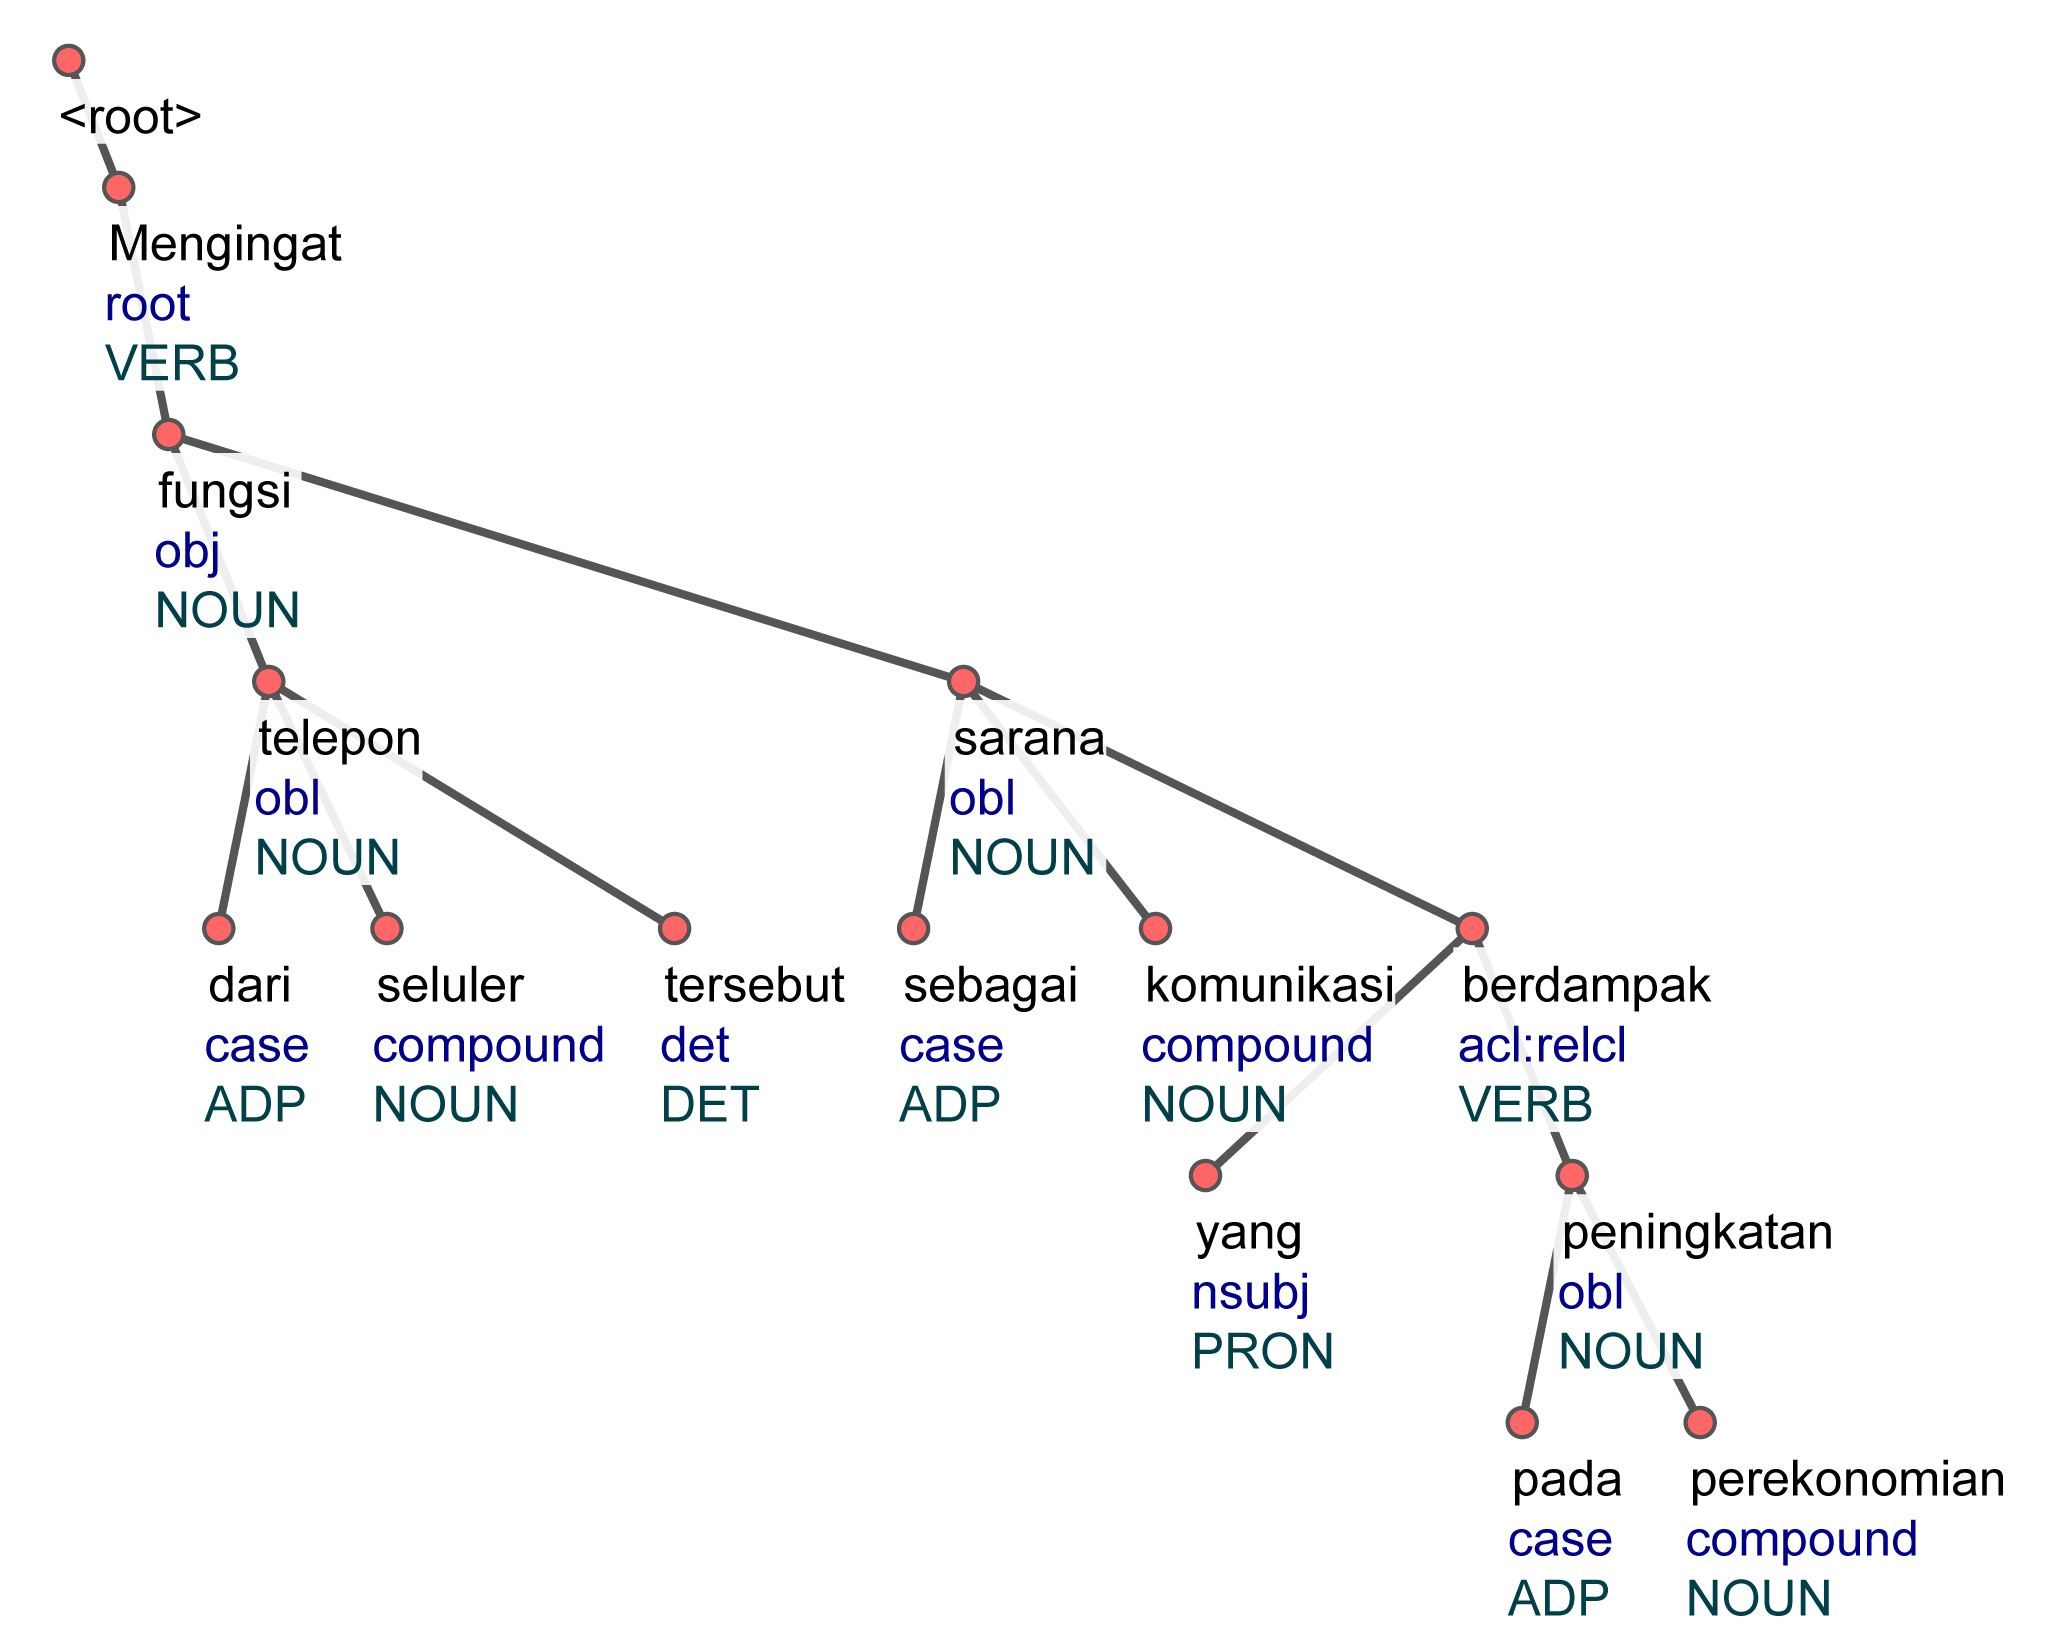
\includegraphics[width=0.8
	\textwidth] {pics/visualisasi_penguraian.jpg} 
	\caption{Contoh visualisasi penguraian kalimat berdasarkan dependensi} 
\label{fig:visualisasi_penguraian} \end{figure}

Untuk memudahkan langkah analisis kualitatif dan tinjauan secara lebih rinci terhadap tautan-tautan dependensi yang terbentuk pada sebuah kalimat, visualisasi seperti pada \pic~\ref{fig:visualisasi_penguraian} dilakukan secara terpisah. Proses visualisasi ini hanya dilakukan pada kalimat-kalimat yang akan dilihat lebih rinci sebagai contoh yang mewakili hasil temuan dengan bantuan kerangka kerja UDPipe \citep{udpipe2017}. Pada kalimat contoh ini, terlihat bahwa kalimat tersebut memiliki akar verbal \textit{mengingat} yang simpai pusatnya hanya terdiri dari satu tautan, yaitu \textit{mengingat fungsi} dengan hubungan tautan $obj$ atau obyek. Penelitian ini merupakan penelitian terhadap penggunaan tuturan nyata sehingga meskipun beberapa kalimat yang ditemukan terlihat seperti klausa terikat saja, atau tampak seperti kalimat yang tidak gramatikal, semua kalimat tetap dianalisis tanpa koreksi atau manipulasi.

\begin{center}
\begin{table} \caption{Penggalan anotasi panjang dan rata-rata jarak dependensi}\label{tab:dl_mdd}
\begin{tiny}
  \begin{tabulary}{1\textwidth}{| L | L | L | L | L | L | L | L |}
  \hline
type & sentence & dl & sum\textunderscore dl & dl\textunderscore positive & dl\textunderscore negative & mdd \\ \hline
tulis & Mengingat fungsi dari telepon seluler tersebut sebagai sarana komunikasi yang berdampak pada peningkatan perekonomian & 0 & 0 & 0 & 0 & 0.00 \\ \hline
tulis & Mengingat fungsi dari telepon seluler tersebut sebagai sarana komunikasi yang berdampak pada peningkatan perekonomian & 1 & 1 & 1 & 0 & 0.08 \\ \hline
tulis & Mengingat fungsi dari telepon seluler tersebut sebagai sarana komunikasi yang berdampak pada peningkatan perekonomian & -1 & 2 & 1 & -1 & 0.15 \\ \hline
tulis & Mengingat fungsi dari telepon seluler tersebut sebagai sarana komunikasi yang berdampak pada peningkatan perekonomian & 2 & 4 & 3 & -1 & 0.31 \\ \hline
tulis & Mengingat fungsi dari telepon seluler tersebut sebagai sarana komunikasi yang berdampak pada peningkatan perekonomian & 1 & 5 & 4 & -1 & 0.38 \\ \hline
tulis & Mengingat fungsi dari telepon seluler tersebut sebagai sarana komunikasi yang berdampak pada peningkatan perekonomian & 2 & 7 & 6 & -1 & 0.54 \\ \hline
tulis & Mengingat fungsi dari telepon seluler tersebut sebagai sarana komunikasi yang berdampak pada peningkatan perekonomian & -1 & 8 & 6 & -2 & 0.62 \\ \hline
tulis & Mengingat fungsi dari telepon seluler tersebut sebagai sarana komunikasi yang berdampak pada peningkatan perekonomian & 6 & 14 & 12 & -2 & 1.08 \\ \hline
tulis & Mengingat fungsi dari telepon seluler tersebut sebagai sarana komunikasi yang berdampak pada peningkatan perekonomian & 1 & 15 & 13 & -2 & 1.15 \\ \hline
tulis & Mengingat fungsi dari telepon seluler tersebut sebagai sarana komunikasi yang berdampak pada peningkatan perekonomian & -1 & 16 & 13 & -3 & 1.23 \\ \hline
tulis & Mengingat fungsi dari telepon seluler tersebut sebagai sarana komunikasi yang berdampak pada peningkatan perekonomian & 3 & 19 & 16 & -3 & 1.46 \\ \hline
tulis & Mengingat fungsi dari telepon seluler tersebut sebagai sarana komunikasi yang berdampak pada peningkatan perekonomian & -1 & 20 & 16 & -4 & 1.54 \\ \hline
tulis & Mengingat fungsi dari telepon seluler tersebut sebagai sarana komunikasi yang berdampak pada peningkatan perekonomian & 2 & 22 & 18 & -4 & 1.69 \\ \hline
tulis & Mengingat fungsi dari telepon seluler tersebut sebagai sarana komunikasi yang berdampak pada peningkatan perekonomian & 1 & 23 & 18 & -5 & 1.77 \\ \hline
  \end{tabulary}  
\end{tiny}
\end{table}
\end{center}

Tahap selanjutnya melibatkan proses anotasi yang berkaitan dengan panjang dan jarak tautan dependensi sebuah kalimat pada tabel hasil penguraian kalimat. \tab~\ref{tab:dl_mdd} merupakan tabel hasil anotasi terhadap salah satu kalimat di dalam korpus data. Anotasi ini dihasilkan melalui penghitungan DL dan MDD seperti yang dijabarkan pada Bab 2 dan rumus penghitungan yang dijabarkan pada Bab 3. DL menekankan pada total jarak-jarak dependensi yang didapatkan dari semua tautan dependensi dalam sebuah kalimat, sedangkan MDD menekankan pada rata-rata jarak dependensi antara dua konstituen dalam sebuah kalimat. Meskipun memiliki prinsip mendasar yang serupa, diduga ada perbedaan informasi yang berarti antara kedua pendekatan ini sehingga keduanya digunakan dalam penelitian ini. Penelitian ini tidak melakukan eksplorasi terhadap perbedaan pendekatan DL dan MDD ataupun menentukan pendekatan mana yang lebih optimal dalam mengilustrasikan efisiensi memori kerja melalui struktur sintaksis kalimat. Meskipun begitu, hasil penerapan kedua pendekatan dalam penelitian ini dapat berkontribusi dalam menunjukkan pada kondisi mana kedua pendekatan tersebut berbeda.

\tab~\ref{tab:dl_mdd} memperlihatkan penghitungan DL dan MDD untuk kalimat \textit{Mengingat fungsi dari telepon seluler tersebut sebagai sarana komunikasi yang berdampak pada peningkatan perekonomian}. Dengan jumlah konstituen 14, kalimat ini memiliki DL sejauh 23 dan MDD sejauh 1,77 konstituen. Hasil ini menunjukkan total jarak dari tautan-tautan dependensi (total Jarak Dependensi atau DD antarkonstituen) dalam kalimat tersebut berjumlah 23 dengan rata-rata jarak dependensi antara dua konstituen yang memiliki jarak tautan langsung sejauh 1,77 konstituen. Pada tabel tersebut terlihat bahwa DL juga dipisahkan menjadi dua berdasarkan direksionalitas induknya. DL positif menggambarkan kondisi relasi diawali induk yang berarti  akar atau induk direalisasikan sebelum konstituen terikat. Sebaliknya, DL negatif menggambarkan kondisi relasi diakhiri induk yang berarti akar atau induk direalisasikan setelah konstituen terikat. Analisis hubungan DL positif dan negatif ini memiliki dua bagian. Bagian pertama adalah tinjauan terhadap tautan antara dua konstituen yang memiliki tautan langsung tanpa memperhitungkan konteks frasa, klausa, atau kalimat tempat kedua konstituen tesebut berada. Analisis bagian kedua adalah tinjauan terhadap tautan antara dua konstituen di mana salah satu konstituen tersebut adalah akar verbal (simpai pusat) dan semua simpai cabang konstituen tersebut dianggap mengikuti induknya. Pada kalimat kompleks yang memiliki lebih dari satu klausa, tautan dependensi utama ini dapat membawa satu klausa atau lebih di dalamnya. Sebagai contoh, jika terdapat satu tautan dependensi utama yang negatif, dan dalam simpai cabang tersebut terdapat dua klausa, kedua klausa tersebut harus disimpan di dalam memori kerja terlebih dahulu hingga akar direalisasikan. Oleh sebab itu, posisi simpai cabang menentukan bagaimana seluruh informasi yang dikandungnya diproses. Analisis ini berangkat dari asumsi bahwa bahasa Indonesia cenderung memilih bentuk relasi diawali induk yang diambil dari indikasi dari teori struktur frasa yang mengungkapkan banyaknya kondisi di mana kata kepala akan mendahului konstituen terikatnya (\citealp{kridalaksana2002struktur, sneddon2010indonesian}).

\begin{figure}
	\centering 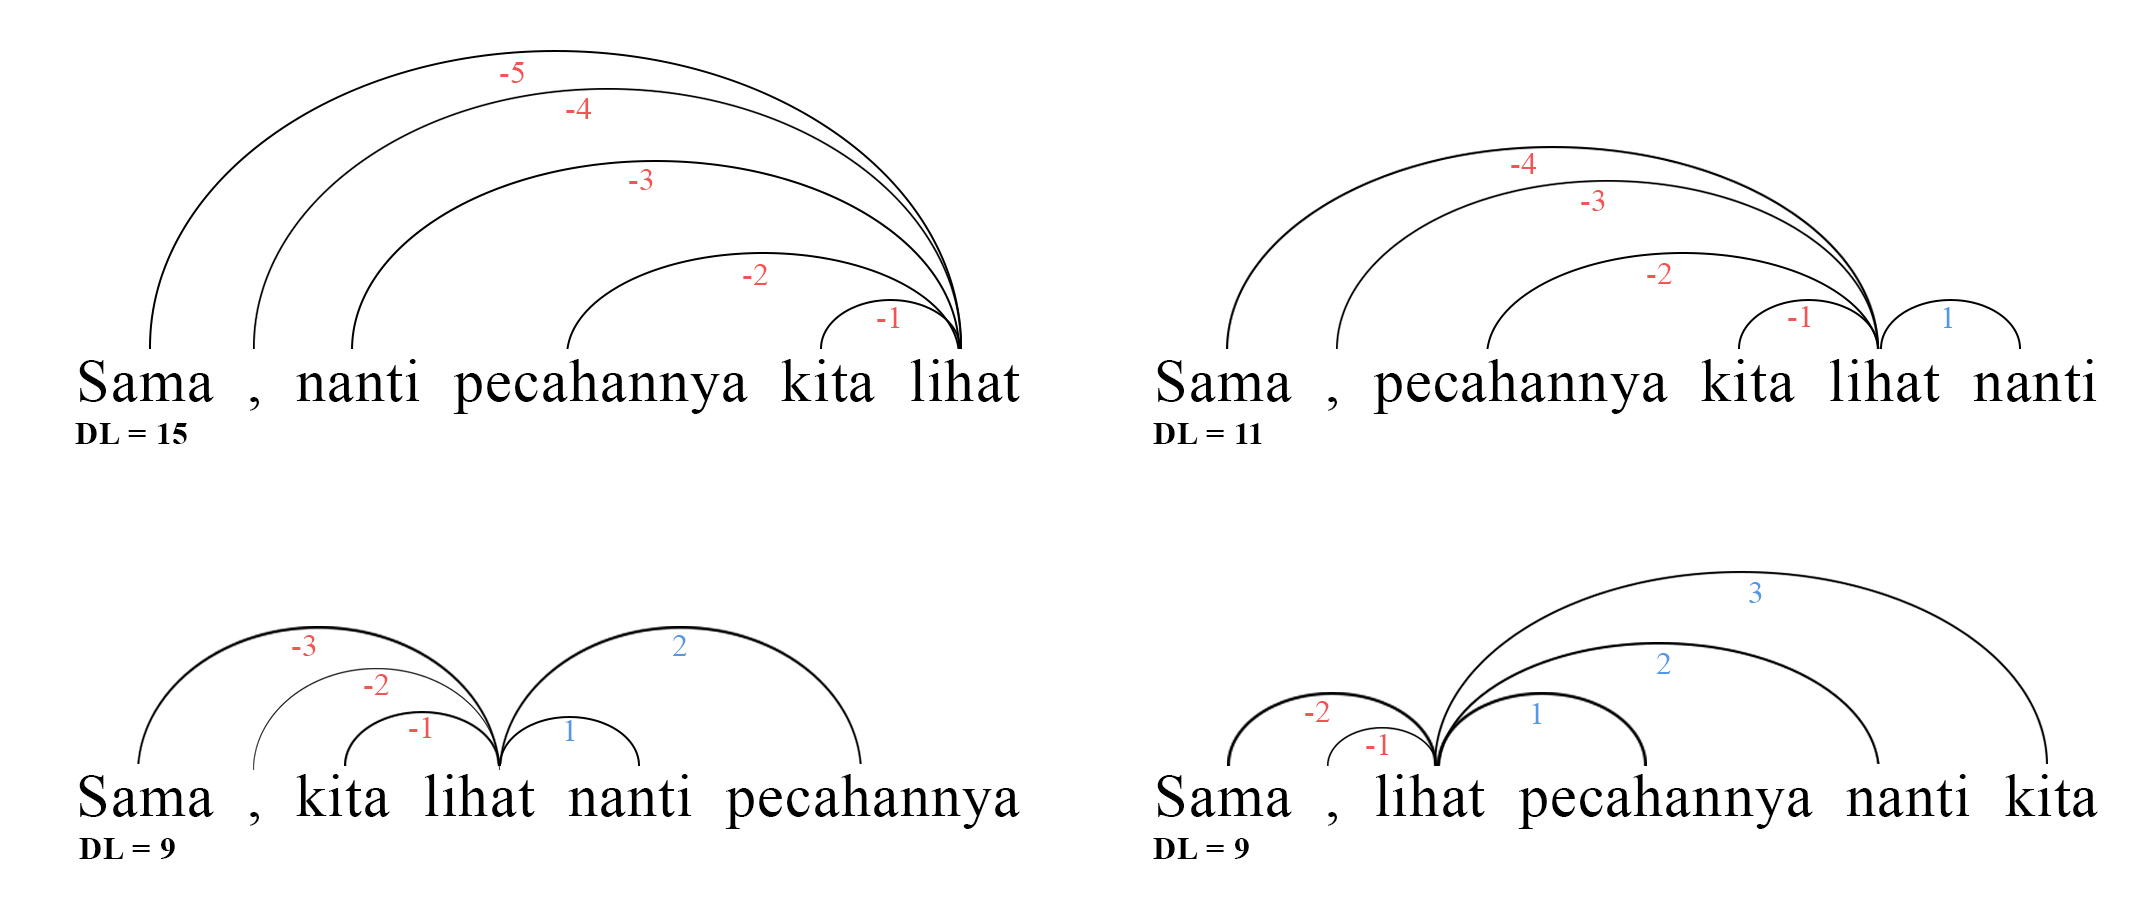
\includegraphics[width=0.8
	\textwidth] {pics/percobaan_acak.jpg} 
	\caption{Contoh hasil percobaan acak} 
\label{fig:percobaan_acak} 
\end{figure}

Berikutnya, langkah yang dilakukan setelah mendapatkan tabel hasil penguraian ini adalah percobaan acak dengan mengadopsi prinsip langkah-langkah algoritma acak \textit{Free Word Order Baseline} \citep{futrell2015large}. \textit{Free Word Order Baseline} merupakan pendekatan yang dilakukan \cite{futrell2015large} dalam menguji hipotesis adanya Pengurangan Panjang Dependensi (DLM). Pada tahap ini tidak dilakukan perbandingan untuk menguji hipotesis Pengurangan Jarak Dependensi (DDM) karena variabel pembagi, yang dalam hal ini adalah jumlah tautan, tidak berubah sehingga akan menghasilkan gambaran yang serupa dengan tinjauan terhadap DLM. Dari kalimat-kalimat yang telah diurai, percobaan ini menghasilkan 100 kombinasi struktur kalimat dengan mempertahankan kaidah tautan dependensi sesuai hasil observasi. \pic~\ref{fig:percobaan_acak} memperlihatkan tiga contoh hasil percobaan acak terhadap kalimat \textit{Sama, nanti pecahannya kita lihat} serta perbedaan DL yang didapatkan tiga kombinasi struktur lainnya. Percobaan acak ini dilakukan terhadap semua kalimat yang berada pada kategori jumlah konstituen dengan frekuensi terbanyak. Berdasarkan klasifikasi kalimat terhadap kedua korpus data dan tahap pertama analisis, frekuensi jumlah konstituen terbanyak pada setiap klasifikasi kalimat adalah 10 konstituen (ragam tulis) dan 5 konstituen (ragam lisan) untuk klasifikasi kalimat pendek (\textless= 10 konstituen), 14 konstituen (ragam tulis) dan 12 konstituen (ragam lisan) untuk klasifikasi kalimat menengah (11-20 konstituen), serta 21 konstituen (ragam tulis) dan 22 konstituen (ragam lisan) untuk klasifikasi kalimat panjang (\textgreater 20 konstituen). 

Merujuk pada penjelasan dalam tinjauan pustaka pada Bab 2, bahasa Indonesia memiliki urutan kata yang cenderung bebas, dan beberapa kasus menunjukkan pertukaran kata maupun klausa tidak mengubah makna kalimat \citep{sneddon2010indonesian}. Dalam penelitiannya, \cite{futrell2015large} menunjukkan kedekatan hasil data observasi bahasa Indonesia dengan DL minimum dengan menggunakan pendekatan ini berdasarkan korpus data yang berisi artikel penelitian. Temuan ini memberikan indikasi bahwa penerapan kebebasan urutan kata tidak hanya terjadi pada kalimat yang dianggap gramatikal, tetapi terutama pada tuturan nyata dalam kehidupan sehari-hari (data penampilan bahasa). Kebebasan terhadap aturan ini dan asumsi bahwa penutur bahasa Indonesia memanfaatkan kebebasan ini merupakan dasar utama pemilihan pendekatan \textit{Free Word Order Baseline}. Hal ini dikarenakan pendekatan tersebut menghasilkan hasil kombinasi struktur kalimat dengan panjang paling minimal dan maksimal sehingga sangat menarik untuk melihat posisi tuturan nyata yang didapat melalui observasi terhadap kemungkinan-kemungkinan kombinasi struktur yang terbentuk. 

Tahap terakhir dari analisis penelitian ini merupakan analisis kualitatif untuk melihat perilaku valensi konstituen yang difokuskan pada valensi akar verbal pada simpai pusat kalimat. Verba sebagai akar kalimat ditemukan sebanyak 84,61\% atau sebanyak 7874 kalimat pada data ragam tulis dan 70,91\% atau sebanyak 7239 kalimat pada data ragam lisan. Oleh sebab itu, bentuk ini merupakan bentuk kalimat dalam kedua korpus data. Analisis ini dilakukan untuk melihat adanya strategi yang menyebabkan terjadinya DLM dan DDM pada tingkat dependensi paling utama (simpai pusat) serta perbedaan karakter yang mungkin muncul antara kedua jenis ragam bahasa. Analisis kualitatif juga dilakukan pada temuan yang didapat pada tahap-tahap sebelumnya untuk menguraikan struktur kalimat yang mungkin memberikan informasi lebih mengenai kecenderungan penutur dalam membentuk kalimat yang efisien dari segi dependensi.

%-----------------------------------------------------------------------------%
\section{Panjang dependensi kalimat dan rata-rata jarak dependensi antarkonstituen data ragam tulis dan lisan}
%-----------------------------------------------------------------------------%
Pada bagian analisis penelitian ini, kedua pendekatan untuk menghitung DL dan MDD digunakan karena diduga masing-masing memberikan informasi yang berbeda atau menunjukkan perbedaan karakter pada kondisi tertentu. Kedua penghitungan ini dilakukan terhadap setiap kalimat dalam korpus data jurnalistik ragam lisan dan tulis. Secara garis besar, ada perbedaan yang cukup jelas terlihat dalam kedua paparan grafik nilai DL dan nilai MDD antara korpus data ragam tulis dan data ragam lisan.

%-----------------------------------------------------------------------------%
\subsection{Perbandingan panjang dependensi kalimat data ragam tulis dan lisan}
%-----------------------------------------------------------------------------%

Pada pendekatan penghitungan panjang dependensi kalimat (DL) yang diadopsi dari penelitian \cite{futrell2015large}, seluruh nilai tautan dependensi dalam sebuah kalimat dijumlahkan sehingga DL yang dihasilkan cukup sensitif dan berbanding linear dengan jumlah konstituen dalam kalimat. Pada \pic~\ref{fig:lisantulis_DL}, sumbu $x$ merepresentasikan panjang kalimat atau jumlah konstituen dan sumbu $y$ merepresentasikan DL dalam sebuah kalimat. Berdasarkan grafik ini, dapat dicermati bahwa terjadi perubahan pada kedua garis regresi antara ragam tulis dan lisan. Perbandingan umum ini dilakukan tanpa melihat lebih dalam persebaran data terkait jumlah konstituen dalam kalimat atau tanpa memperhitungkan klasifikasi panjang kalimat. Berdasarkan grafik DL ini, terlihat bahwa mayoritas jumlah konstituen dalam kalimat pada kedua korpus data berada di bawah 40 konstituen. Pada area di bawah 40 konstituen, garis regresi data ragam tulis berada di bawah garis regresi data ragam lisan. Namun, pada area di atas 40 konstituen, garis regresi menunjukkan perbandingan terbalik secara drastis. Secara umum, rata-rata DL adalah 42,61 untuk data ragam tulis dan 24,36 untuk data ragam lisan. 

\begin{figure}
	\centering 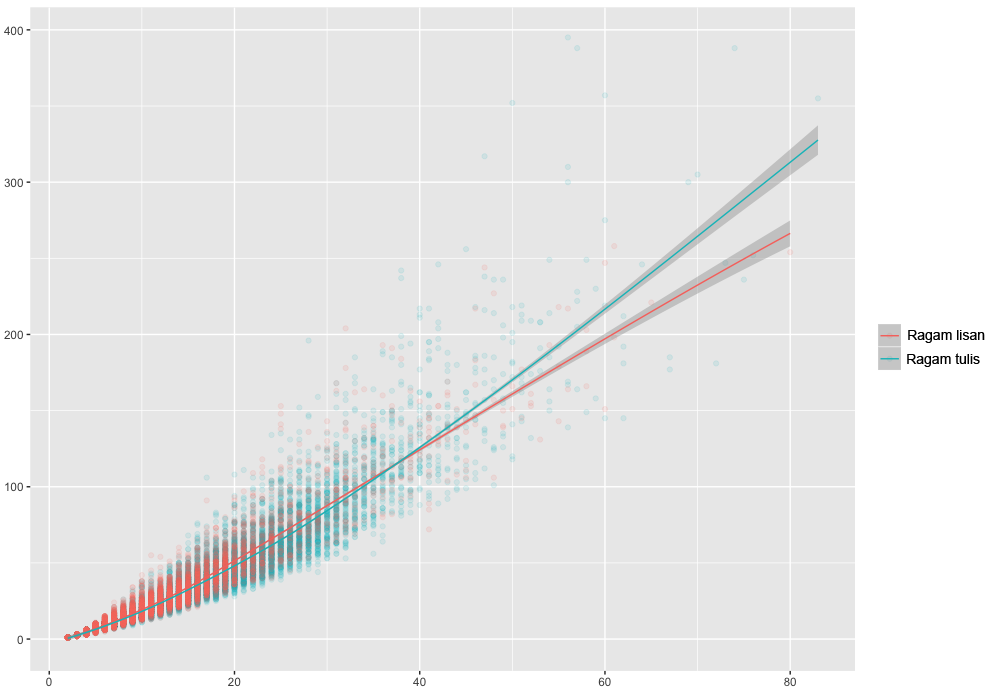
\includegraphics[width=1
	\textwidth] {pics/lisantulis_DL.png} 
	\caption{Grafik panjang dependensi data ragam tulis dan lisan} 
\label{fig:lisantulis_DL} 
\end{figure}

Tanpa memperhitungkan klasifikasi panjang kalimat, hasil rata-rata DL pada \pic~\ref{fig:lisantulis_DL} menunjukkan adanya perbedaan yang signifikan bahwa ragam lisan akan menghasilkan jumlah nilai tautan dependensi yang lebih kecil. Seperti yang terlihat pada garis regresi yang terbentuk, hingga panjang kalimat 40 konstituen, garis regresi data ragam tulis terus berada di bawah garis regresi ragam lisan dan terjadi pemusatan data pada panjang kalimat yang mendekati minimum untuk data ragam lisan. Hal ini berarti hal lain yang mempengaruhi panjang dependensi sehingga data ragam lisan dapat menghasilkan rata-rata yang lebih kecil dibandingkan data ragam tulis dilihat dari segi total panjang dependensi dalam sebuah kalimat. Hal ini menunjukkan bahwa dugaan awal ini harus dicermati lebih dalam dengan melihat klasifikasi panjang kalimat yang mungkin akan memberikan informasi tambahan lain dalam menentukan keakuratan hasil tinjauan. 

%-----------------------------------------------------------------------------%
\subsection{Perbandingan rata-rata jarak dependensi antarkonstituen data ragam tulis dan lisan}
%-----------------------------------------------------------------------------%

Berbeda dengan penghitungan DL, rata-rata jarak dependensi antarkonstituen (MDD) didapatkan dengan membagi total panjang dependensi dalam sebuah kalimat dengan jumlah tautan itu sendiri. Penghitungan ini menghasilkan perkiraan rata-rata jarak dependensi sebuah tautan dalam kalimat tersebut sehingga menggambarkan pada umumnya sejauh apa jarak relasi semantik antar dua konstituen. Seperti \pic~\ref{fig:lisantulis_DL}, \pic~\ref{fig:lisantulis_MDD} merupakan paparan MDD untuk semua kalimat pada kedua korpus data (ragam tulis dan lisan). MDD, seperti yang dikemukakan oleh \cite{liu2017dependency}, tidak terlalu sensitif terhadap jumlah konstituen karena merupakan rata-rata jarak per tautan dependensi. Meskipun begitu, berdasarkan grafik MDD ini, pada data dengan jumlah konstituen di bawah 10, MDD masih menunjukkan hasil yang sangat linear terhadap jumlah konstituen. Hal ini mengindikasikan bahwa pada jumlah konstituen yang sedikit, MDD masih memiliki tingkat sensitivitas yang cukup tinggi terhadap panjang kalimat.

\begin{figure}
	\centering 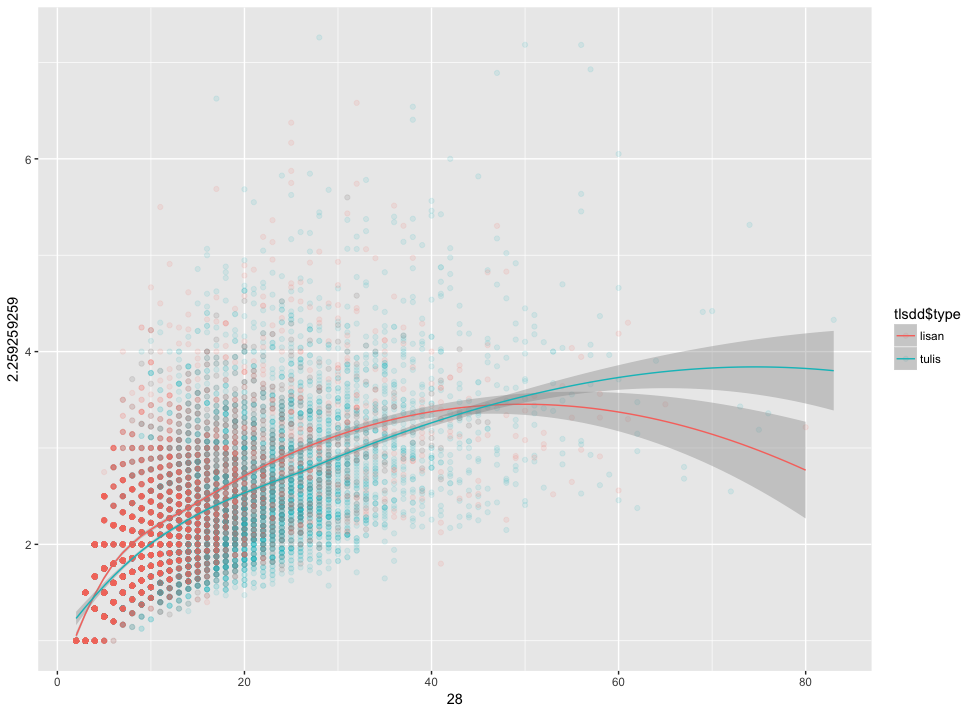
\includegraphics[width=1
	\textwidth] {pics/lisantulis_MDD.png} 
	\caption{Grafik rata-rata jarak dependensi data ragam tulis dan lisan} 
\label{fig:lisantulis_MDD} 
\end{figure}

Apabila DL memberikan gambaran umum mengenai kompleksitas sebuah kalimat karena hanya difokuskan terhadap total panjang dependensi keseluruhan kalimat, MDD dapat lebih memberikan ilustrasi kerja kognisi manusia yang tercermin pada relasi dua buah konstituen dengan kondisi agar kedua konstituen dapat bermakna secara utuh, salah satu harus menunggu yang lain untuk direalisasikan. Pada \pic~\ref{fig:lisantulis_MDD}, dapat disimpulkan bahwa garis regresi untuk korpus data ragam tulis juga berada di bawah garis regresi korpus data ragam lisan dengan panjang kalimat di bawah 40 konstituen namun berbanding terbalik setelah 40 konstituen. Temuan ini menunjukkan konsistensi antara DL dan MDD yang sama-sama menunjukkan bahwa hingga jumlah setidaknya 40 konstituen, kalimat-kalimat dalam data ragam tulis menunjukkan efisiensi yang lebih tinggi dari segi dependensi dibandingkan data ragam lisan. Namun, rata-rata MDD yang didapat dari seluruh kalimat justru memperlihatkan hasil sebaliknya. Rata-rata MDD untuk data ragam lisan adalah 2,05 konstituen dan 2,35 konstituen untuk data ragam tulis. Seperti pada catatan grafik nilai DL sebelumnya, rata-rata ini tidak memperhitungkan klasifikasi panjang kalimat dan pemusatan data ragam tulis pada panjang kalimat yang mendekati minimum yang juga patut diperhitungkan.

%%-----------------------------------------------------------------------------%
\section{Perbandingan data hasil observasi dengan hasil percobaan acak}
%%-----------------------------------------------------------------------------%
Setelah mendapatkan gambaran umum mengenai DL dan MDD untuk kedua korpus data, percobaan acak terhadap kedua korpus data dilakukan untuk melihat apakah kalimat-kalimat dalam data hasil observasi, baik ragam tulis maupun lisan, memiliki kecenderungan untuk menghindari panjang dependensi dan jarak tautan dependensi yang lebih jauh. Berdasarkan hipotesis DLM, \cite{futrell2015large} mengajukan bahwa jika bahasa berevolusi untuk mendukung komunikasi yang lebih mudah, seharusnya urutan kata yang dimanfaatkan penutur dalam tuturan nyata tidak menghasilkan panjang dependensi yang jauh. Hal ini terjadi karena panjang dependensi yang jauh mencerminkan kompleksitas produksi ataupun pemahaman yang lebih tinggi. Percobaan acak dengan pendekatan \textit{Free Word Order Baseline} menghasilkan 100 bentuk urutan konstituen acak untuk setiap kalimat dengan mempertahankan struktur tautan-tautan dependensi yang sama dengan kalimat dalam data observasi. 

Beberapa histogram berikut menunjukkan perbandingan antara DL dari semua kalimat dalam data hasil observasi dengan DL dari hasil percobaan acak dalam data ragam tulis (\pic~\ref{fig:trandomobs}) serta ragam lisan (\pic~\ref{fig:lrandomobs}). Sumbu $x$ menandakan panjang dependensi dan sumbu $y$ menandakan persentase jumlah kalimat yang memiliki DL tersebut. Perbandingan ini dilakukan dengan mengontrol jumlah konstituen sehingga hasil percobaan acak dapat memberikan nilai yang spesifik. \cite{futrell2015large} pernah menampilkan histogram serupa dengan jumlah konstituen sebanyak 12. Berdasarkan penelitiannya, nilai terkecil dari data bahasa Indonesia hasil observasi sangat mendekati nilai minimum dari hasil percobaan acak.

\begin{figure}
\centering

\begin{subfigure}{.45\textwidth}
  \centering
  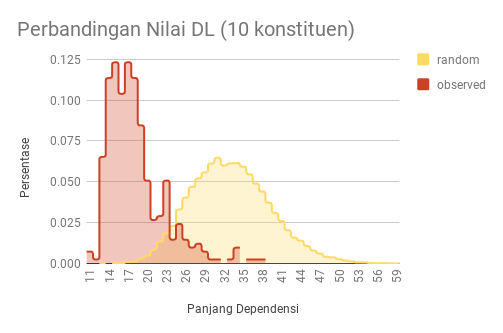
\includegraphics[width=1\linewidth]{pics/t10randomobs.png}
  \caption{10 konstituen}
  \label{fig:t10randomobs} 
\end{subfigure}
%
\begin{subfigure}{.45\textwidth}
  \centering
  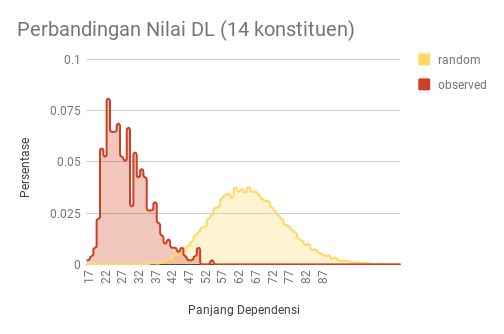
\includegraphics[width=1\linewidth]{pics/t14randomobs.png}
  \caption{14 konstituen}
  \label{fig:t14randomobs} 
\end{subfigure}
%
\begin{subfigure}{.45\textwidth}
  \centering
  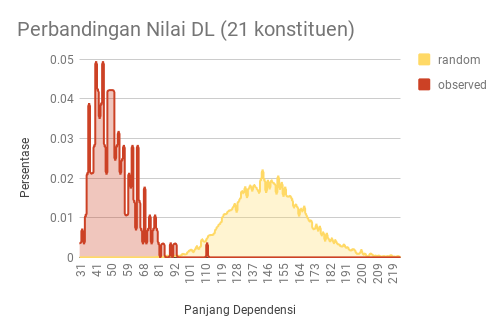
\includegraphics[width=1\linewidth]{pics/t21randomobs.png}
  \caption{21 konstituen}
  \label{fig:t21randomobs} 
\end{subfigure}

\caption{Panjang dependensi data hasil observasi dan hasil percobaan acak untuk panjang kalimat 10,14, dan 21 konstituen pada data ragam tulis}
\label{fig:trandomobs}
\end{figure}

\pic~\ref{fig:trandomobs} memperlihatkan histogram perbandingan DL antara data hasil observasi dengan hasil percobaan acak untuk jumlah konstituen 10, 14, dan 21. Jumlah-jumlah konstituen ini memiliki frekuensi terbanyak yang mewakili setiap kelompok klasifikasi kalimat pada data ragam tulis.  Histogram hasil percobaan acak terlihat jelas membentuk kurva yang lebih rendah dibandingkan dengan kurva yang dibentuk oleh data observasi. Hal ini berarti hasil percobaan acak memiliki distribusi DL yang lebih besar dibandingkan dengan data observasi. Berdasarkan histogram ini, dapat dilihat juga bahwa pada jumlah konstituen yang semakin banyak, irisan antara kurva nilai DL data observasi dan hasil percobaan acak semakin sedikit.

\begin{table}
\begin{center}
\begin{small}
  \caption{Tabel perbandingan rata-rata panjang dependensi data hasil observasi dan hasil percobaan acak untuk data ragam tulis}  \label{tab:perbandingan_DL_tulis}
  \begin{tabular}{ | l | l | l | l |}
    \hline
    	Jumlah konstituen & Rata-rata nilai DL (observasi) & Rata-rata nilai DL (acak) & p-value \\ \hline
	10 & \textbf{18,14} & 33,01 & \textless \0,001 \\ \hline
	14 & \textbf{29,11} & 64,95 & \textless 0,001 \\ \hline
	21 & \textbf{51,59} & 146,67 & \textless 0,001 \\ \hline
  \end{tabular}
  \end{small}
\end{center}
\end{table}

\tab~\ref{tab:perbandingan_DL_tulis} menunjukkan perbedaan rata-rata DL yang cukup jauh antara data hasil observasi dengan hasil percobaan acak untuk data ragam tulis dengan efek yang signifikan pada semua jumlah konstituen (\textit{P} \textless 0,001). Semua histogram dan perbedaan rata-rata tersebut mengkonfirmasi terjadinya DLM pada data hasil observasi ragam tulis sehingga kalimat-kalimat pada korpus tersebut lebih efisien dibandingkan dengan hasil percobaan acaknya.

\begin{figure}
\centering

\begin{subfigure}{.45\textwidth}
  \centering
  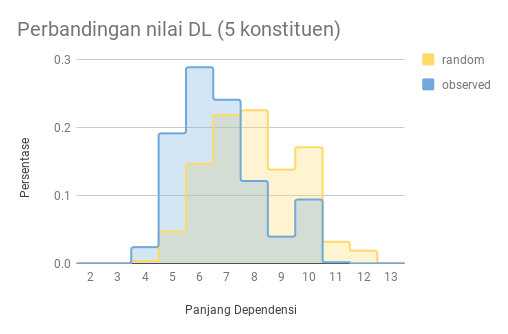
\includegraphics[width=1\linewidth]{pics/l5randomobs.png}
  \caption{5 konstituen}
  \label{fig:l5randomobs} 
\end{subfigure}
%
\begin{subfigure}{.45\textwidth}
  \centering
  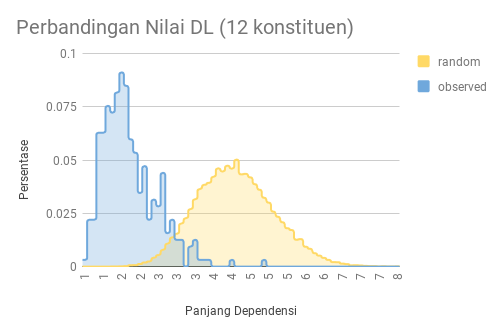
\includegraphics[width=1\linewidth]{pics/l12randomobs.png}
  \caption{12 konstituen}
  \label{fig:l12randomobs} 
\end{subfigure}
%
\begin{subfigure}{.45\textwidth}
  \centering
  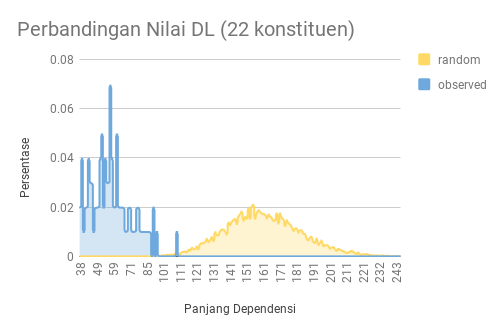
\includegraphics[width=1\linewidth]{pics/l22randomobs.png}
  \caption{22 konstituen}
  \label{fig:l22randomobs} 
\end{subfigure}

\caption{Panjang dependensi data hasil observasi dan hasil percobaan acak untuk panjang kalimat 5,12, dan 22 konstituen pada data ragam lisan}
\label{fig:lrandomobs}
\end{figure}

Sesuai dengan ekspektasi, percobaan acak terhadap data ragam lisan menunjukkan hasil yang serupa dengan percobaan terhadap data ragam tulis. \pic~\ref{fig:lrandomobs} merupakan histogram perbandingan DL antara data hasil observasi dengan hasil percobaan acak untuk jumlah konstituen 5, 12, dan 22 yang mewakili setiap kelompok klasifikasi kalimat pada data ragam lisan. Histogram hasil percobaan acak untuk ragam lisan juga membentuk kurva yang secara jelas terlihat lebih rendah dan juga menandakan bahwa  acak memiliki distribusi DL yang lebih besar dibandingkan dengan data hasil observasi. Bahkan untuk jumlah konstituen 5 yang tergolong kalimat sangat pendek, data observasi masih memperlihatkan adanya indikasi DLM secara signifikan dengan nilai \textit{P} \textless 0,001. Berdasarkan histogram ini juga dapat dilihat bahwa pada jumlah konstituen yang semakin banyak, irisan antara nilai DL data observasi dan hasil percobaan acak semakin sedikit. Hal ini berarti DLM semakin jelas terlihat pada kalimat yang semakin panjang.

\begin{table}
\begin{center}
\begin{small}
  \caption{Tabel perbandingan rata-rata panjang dependensi data hasil observasi dan hasil percobaan acak untuk data ragam lisan}  \label{tab:perbandingan_DL_lisan}
  \begin{tabular}{ | l | l | l | l |}
    \hline
	 Jumlah konstituen & Rata-rata nilai DL (observasi) & Rata-rata nilai DL (acak) & \textit{p-value} \\ \hline
	 5 & \textbf{6,74} & 7,98 & \textless 0,001 \\ \hline
	 12 & \textbf{24,78} & 47,7 & \textless 0,001 \\ \hline
	 22 & \textbf{58,92} & 160,89 & \textless 0,001 \\ \hline
  \end{tabular}
  \end{small}
\end{center}
\end{table}

Serupa juga dengan percobaan terhadap data ragam tulis, \tab~\ref{tab:perbandingan_DL_lisan} menunjukkan perbedaan rata-rata DL yang cukup jauh antara data hasil observasi dan hasil percobaan acak untuk data ragam lisan dengan efek yang signifikan pada semua jumlah konstituen (\textit{P} \textless 0,001). Berdasarkan semua paparan tersebut, dapat disimpulkan juga bahwa kalimat-kalimat pada data hasil observasi ragam lisan juga lebih efisien dibandingkan hasil percobaan acaknya.

Percobaan acak pada kedua korpus data dengan jumlah konstituen yang berbeda-beda menunjukkan adanya optimasi struktur kalimat pada data hasil observasi sehingga terjadi pengurangan panjang dependensi (DLM) secara menyeluruh. Histogram hasil percobaan acak menunjukkan bahwa pada semua jumlah konstituen, distribusi DL data hasil observasi jauh lebih padat dan mendekati jumlah minimum. Temuan ini sejalan dengan hipotesis penelitian \cite{hawkins2014cross} yang menyebutkan bahwa aturan urutan kata mendasar yang dalam pemahaman penutur akan menghasilkan konstruksi kalimat yang tautan dependensinya lebih pendek dibandingkan alternatif konstruksi yang mungkin ada.

Hipotesis pengurangan panjang atau jarak dependensi (DLM atau DDM) berbicara tentang kecenderungan manusia untuk mendekatkan kata-kata yang memiliki relasi semantik. Pendekatan ini dapat dilakukan dengan menerapkan beberapa strategi seperti yang telah dibahas pada penelitian-penelitian terdahulu (\citealp{jaeger2006redundancy, gildea2015human}). Dalam ranah sintaksis, strategi pendekatan-kata-kata ini termasuk melalui penyusunan urutan kata dan pengurangan kata dalam kalimat (yang mungkin diakibatkan oleh pengurangan unsur yang repetitif ataupun hal yang lain). Berdasarkan tahap pertama analisis, yaitu percobaan acak dengan menggunakan \textit{Free Word Order Baseline} \citep{futrell2015large}, dihasilkan 100 kemungkinan struktur kalimat yang tidak memiliki aturan urutan kata tertentu. Percobaan ini mendukung hipotesis bahwa terjadi DLM pada kedua korpus data (ragam tulis maupun ragam lisan) secara signifikan (\textit{P} \textless 0,001). 

Temuan DLM ini juga berkaitan dengan pengurangan jarak dependensi (DDM) karena percobaan acak tidak mengubah jumlah konstituen dalam kalimat yang sama sehingga variabel pembagi DL sebuah kalimat tidak berubah. Temuan ini menandakan bahwa struktur kalimat-kalimat dalam data hasil observasi pada kedua ragam memperlihatkan struktur yang lebih optimal dari segi dependensi dalam menghasilkan DL yang lebih pendek dibandingkan kemungkinan struktur lain yang terbentuk. Perlu ditekankan bahwa struktur yang optimal ini dinilai dari segi dependensi dan bukan dari segi tata bahasa. Hal ini berarti terlepas dari standar gramatikal dan keberterimaannya, variasi struktur kalimat yang ada dalam kedua korpus rata-rata cukup mengoptimalkan memori kerja dan mengindikasikan kemudahan untuk berkomunikasi. Penentuan apakah sebuah struktur optimal, gramatikal, serta mudah dipahami berada di luar batasan penelitian ini. Metodologi lain seperti uji persepsi perlu dilakukan untuk mendapatkan temuan yang akurat. Penilaian dan pengukuran struktur yang lebih optimal dari segi produksi maupun pemahaman berada di luar batasan penelitian ini, sehingga perlu diadakan penelitian lebih lanjut yang melibatkan metodologi transdisipliner dengan ilmu kognitif serta uji persepsi.

%%-----------------------------------------------------------------------------%
\section{Persebaran kalimat dan kaitannya terhadap panjang dependensi kalimat dan rata-rata jarak dependensi antarkonstituen}
%%-----------------------------------------------------------------------------%

Pada \pic~\ref{fig:lisantulis_DL}  dan \pic~\ref{fig:lisantulis_MDD} dalam pembahasan sebelumnya, terlihat jelas adanya perbedaan persebaran kalimat pada kedua korpus data terkait dengan panjang kalimat atau jumlah konstituen. Gambaran umum yang didapatkan dan garis regresi yang ditunjukkan pada kedua gambar tersebut menimbulkan pertanyaan yang hanya dapat dijawab melalui analisis dengan memperhitungkan panjang kalimatnya. Berdasarkan korpus data yang terkumpul, persebaran kalimat pada kedua ragam berbeda secara signifikan. 

\begin{table}
\begin{center}
\begin{small}
   \caption{Persentase kalimat pada tabel klasifikasi jumlah konstituen}  \label{tab:presentase_kalimat}
  \begin{tabular}{ |p{3cm} | p{3cm} | p{3cm} | p{3cm} |}
    \hline
 & Kalimat pendek \newline (\textless=10 konstituen) & Kalimat menengah (11-20 konstituen) & Kalimat panjang (\textgreater20 konstituen) \\ \hline
Data Ragam Tulis & 23,33\% & 45,54\% & 31,13\% \\ \hline
Data Ragam Lisan & 59,49\% & 29,16\% & 11,35\% \\ \hline
  \end{tabular}
  \end{small}
\end{center}
\end{table}

Pada data ragam tulis, sebanyak 45,54\% kalimat berada pada klasifikasi kalimat menengah (\tab~\ref{tab:presentase_kalimat}). Klasifikasi kalimat pendek dan panjang pada ragam tulis memiliki jumlah kalimat yang tidak jauh berbeda. Sementara itu, sebanyak 59,49\% kalimat pada data ragam lisan berada pada klasifikasi kalimat pendek dan menurun secara drastis pada klasifikasi kalimat menengah dan panjang.  

\begin{figure}
	\centering 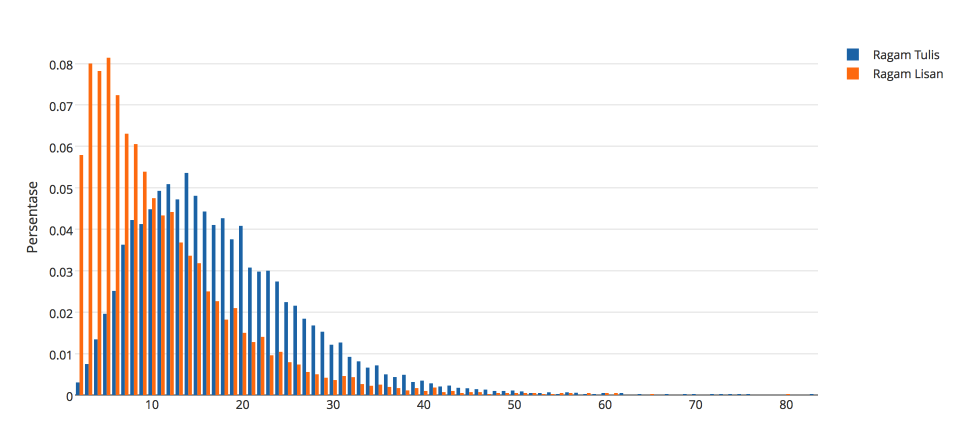
\includegraphics[width=1
	\textwidth] {pics/Jumlah_kata.png} 
	\caption{Diagram perbandingan jumlah konstituen data ragam tulis dan lisan} 
	\label{fig:jumlah_kata} 
\end{figure}

Seperti yang terlihat pada \pic~\ref{fig:jumlah_kata}, terdapat kepadatan yang sangat tinggi pada panjang kalimat di bawah 10 konstituen untuk data ragam lisan, sementara kepadatan tertinggi pada data ragam lisan terletak pada kalimat dengan panjang menengah. Hal ini memperlihatkan bahwa persebaran panjang kalimat pada kedua korpus tidak boleh dihiraukan dalam menganalisis kaitannya dengan panjang dan jarak dependensi. Panjang kalimat dengan frekuensi terbanyak pada data ragam tulis adalah 14 konstituen. Sementara itu, frekuensi terbanyak yang ditemukan pada ragam lisan adalah panjang kalimat 5 konstituen.

%%-----------------------------------------------------------------------------%
\subsection{Pemusatan data ragam lisan pada klasifikasi kalimat pendek (\textless= 10 konstituen)}
%%-----------------------------------------------------------------------------%
Pemusatan data pada klasifikasi kalimat pendek (\textless= 10 konstituen) pada data ragam lisan cukup besar hingga melebihi 50\% dari total jumlah kalimat dalam korpus tersebut. Hal ini berdampak pada perbandingan rata-rata DL serta MDD antara data ragam tulis dan lisan pada kelompok klasifikasi tersebut (\tab~\ref{tab:DL_MDD_pendek}).

\begin{table}
\begin{center}
\begin{small}
\caption{Perbandingan rata-rata panjang dan rata-rata jarak dependensi pada klasifikasi kalimat pendek }\label{tab:DL_MDD_pendek}
  \begin{tabular}{ | p{3.2cm} | p{3.2cm} | p{3.2cm} | p{2cm} |}
    \hline
 & Kalimat pendek \newline (\textless =10 konstituen) \newline Data ragam tulis & Kalimat pendek \newline (\textless =10 konstituen) \newline Data ragam lisan & \textit{p-value} \\ \hline
 Rata-rata nilai DL & 11,85 & \textbf{8,76} & \textless 0,001 \\ \hline
 Rata-rata nilai MDD & 1,792 & \textbf{1,687} & \textless 0,001 \\ \hline
 Rata-rata jumlah konstituen & 7,356 & \textbf{5,708} & \textless 0,001 \\ \hline
 Jumlah kalimat & 2220 & 6073 & -- \\ \hline
   \end{tabular}
   \end{small}
\end{center}
\end{table}

Berdasarkan \tab~\ref{tab:DL_MDD_pendek}, DL dan MDD data ragam lisan lebih pendek dibandingkan data ragam tulis pada klasifikasi kalimat pendek secara signifikan. Berbeda dengan \pic~\ref{fig:lisantulis_DL}  dan \pic~\ref{fig:lisantulis_MDD} yang tidak memperhitungkan klasifikasi panjang kalimat, terutama karena DL berkorelasi cukup linear terhadap panjang kalimat, rata-rata DL pada data ragam lisan dalam klasifikasi ini adalah 8,76. Hasil ini lebih pendek dibandingkan dengan hasil yang didapatkan dari data ragam tulis karena pemusatan jumlah konstituen yang mendekati minimum pada data ragam lisan akan mempengaruhi hasil yang didapat. Hal ini dapat dilihat dari perbandingan rata-rata jumlah konstituen dan jumlah kalimat yang muncul pada klasifikasi ini dengan perbedaan yang signifikan. Meskipun jumlah kalimat data ragam lisan pada klasifikasi ini jauh lebih banyak, rata-rata jumlah konstituen dalam satu kalimat lebih sedikit dibandingkan data ragam tulis.  Berkaitan dengan pemusatan data tersebut, rata-rata MDD data ragam lisan juga menjadi lebih pendek dibandingkan data ragam tulis. Temuan ini menunjukkan indikasi bahwa penggunaan kalimat pendek menjadi salah satu preferensi (dan mungkin strategi)  untuk meningkatkan efisiensi kalimat dalam percakapan lisan. Dalam beberapa kasus di korpus data ragam lisan, ditemukan kalimat-kalimat yang sebenarnya merupakan klausa terikat yang berdiri sendiri sebagai sebuah kalimat utuh dan lepas dari klausa utama yang mungkin berada pada kalimat-kalimat sebelumnya. Seperti contoh, kalimat-kalimat ini banyak ditemukan ditandai dengan konjungsi \textit{dan} pada posisi pertama. 

\begin{table}
\begin{center}
\begin{small}
\caption{Perbandingan panjang dependensi kalimat dengan panjang kurang dan lebih dari 5 konstituen pada klasifikasi kalimat pendek}\label{tab:DL_5}
  \begin{tabular}{ | p{3.2cm} | p{3.2cm} | p{3.2cm} | p{2cm} |}
    \hline
Jumlah konstituen & Data ragam tulis & Data ragam lisan & \textit{p-value} \\ \hline
\textless= 5 konstituen & 4,54 & \textbf{3,92} & \textless 0,001 \\ \hline
6-10 konstituen & 13,75 & 13,6 & \textgreater 0,05 \\ \hline
   \end{tabular}
   \end{small}
\end{center}
\end{table}

\begin{table}
\begin{center}
\begin{small}
\caption{Perbandingan rata-rata jarak dependensi kalimat dengan panjang kurang dan lebih dari 5 konstituen pada klasifikasi kalimat pendek}\label{tab:MDD_5}
  \begin{tabular}{ | p{3.2cm} | p{3.2cm} | p{3.2cm} | p{2cm} |}
    \hline
Rentang & Data ragam tulis & Data ragam lisan & \textit{p-value} \\ \hline
\textless= 5 konstituen & 1,443 & \textbf{1,402} & \textless 0,05 \\ \hline
6-10 konstituen & \textbf{1,883} & 1,972 & \textless 0,001 \\ \hline
   \end{tabular}
   \end{small}
\end{center}
\end{table}

Kepadatan data ragam lisan yang sangat tinggi pada klasifikasi ini memunculkan analisis tambahan untuk melihat perbandingan yang terjadi di dalam klasifikasi ini. Sebelumnya, \cite{wang2017effects} menemukan bahwa MDD ragam teks yang lebih formal lebih kecil dibandingkan ragam teks yang ditujukan untuk ujaran lisan mulai dari panjang kalimat sebanyak 6 konstituen. Dari temuan ini, analisis tambahan dilakukan untuk meninjau perbandingan DL dan MDD pada panjang kalimat kurang dan lebih dari 5 konstituen. \tab~\ref{tab:DL_5} memperlihatkan bahwa perbedaan yang signifikan terkait total panjang dependensi sebuah kalimat hanya ditemukan pada klasifikasi panjang kalimat kurang dari atau sama dengan 5 konstituen. Namun, \tab~\ref{tab:MDD_5} memperlihatkan perbedaan yang signifikan terkait rata-rata jarak dependensi antara dua konstituen dalam kalimat pada kedua sub-klasifikasi, namun berbanding terbalik. Data ragam lisan dengan panjang kalimat kurang dari atau sama dengan 5 konstituen menunjukkan efisiensi yang lebih tinggi, tetapi mulai 6 konstituen, ragam tulis justru memperlihatkan efisiensi yang lebih tinggi dari segi jarak antara dua konstituen.

\begin{figure}
\centering

\begin{subfigure}{.3\linewidth}
  \centering
  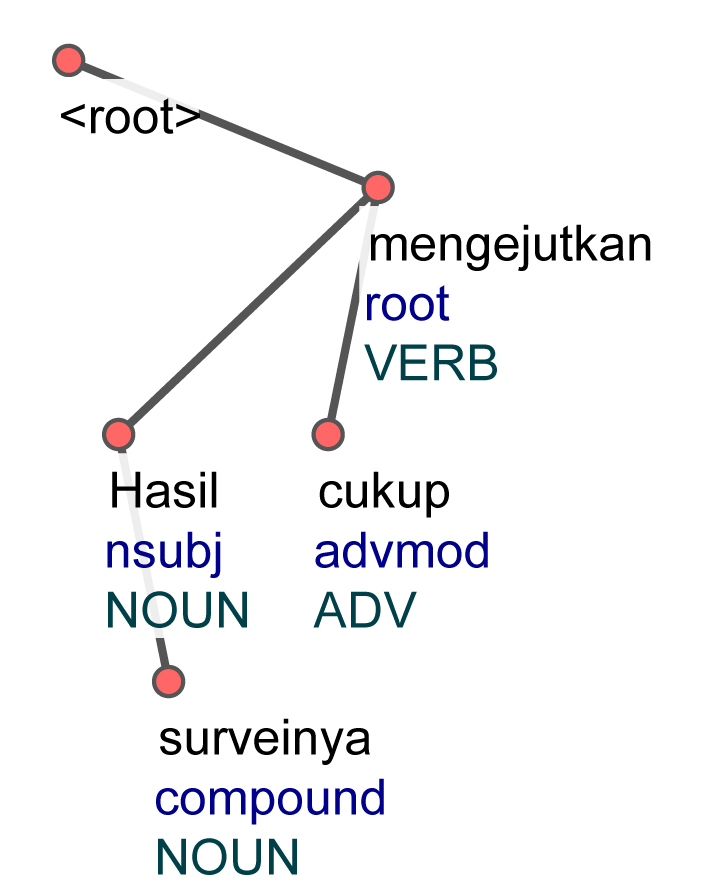
\includegraphics[width=1\linewidth] {pics/ts662.jpg} 
	\caption{T4}
	\label{fig:ts662} 
\end{subfigure}
%
\begin{subfigure}{.35\linewidth}
  \centering
  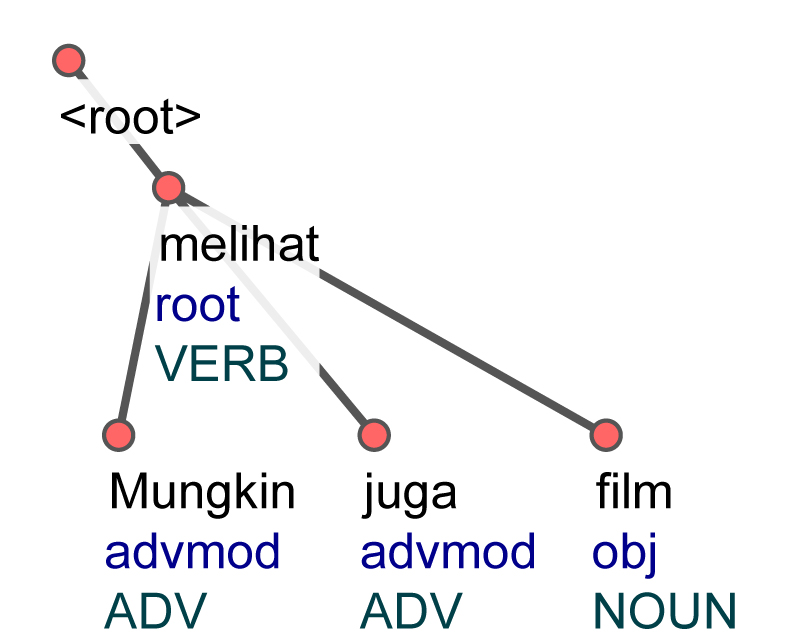
\includegraphics[width=1\linewidth]{pics/ls1102.jpg} 
	\caption{L4}
	\label{fig:ls1102} 
\end{subfigure}

\caption{Contoh perbandingan struktur sintaktis pada panjang kalimat 4 konstituen}
\label{fig:struktur4}
\end{figure}

Panjang dan jarak dependensi ditemukan signifikan pada klasifikasi kalimat pendek, terutama pada panjang kalimat kurang dari atau sama dengan 5 konstituen. Pada contoh kalimat T4 (\pic~\ref{fig:ts662}) yang diambil dari ragam tulis dan kalimat L4 (\pic~\ref{fig:ls1102}) yang diambil dari ragam lisan, perbedaan yang jelas terlihat adalah tidak adanya aktor pelaku pada kalimat L4. Tingkat atau level dependensi yang semakin ke bawah antara dua kalimat tersebut berbeda di mana tingkat kedalaman dependensi T4 lebih banyak. DL dan MDD pada kalimat T4 (\pic~\ref{fig:ts662}) adalah 5 dan 1,67, sementara pada kalimat L4 (\pic~\ref{fig:ls1102}) adalah 4 dan 1,33. Namun, karena jumlah konstituen yang sangat sedikit, perbedaan struktur sintaktis tidak terlalu signifikan secara visual sehingga kurang bisa diasumsikan bahwa ada perbedaan karakteristik yang mendasar antara kedua ragam. 

%%-----------------------------------------------------------------------------%
\subsection{Perbedaan signifikansi panjang dan rata-rata jarak dependensi pada klasifikasi kalimat menengah (11-20 konstituen)}
%%-----------------------------------------------------------------------------%
Pada kelompok klasifikasi kalimat menengah dengan panjang kalimat sebanyak 11 hingga 20 konstituen, terlihat adanya perbedaan dalam perbandingan nilai-nilai di antara kedua ragam. Pada klasifikasi ini ditemukan perbandingan terbalik antara rata-rata DL dan MDD pada kedua korpus data (\tab~\ref{tab:DL_MDD_menengah}). Untuk DL, data ragam lisan memiliki rata-rata yang sedikit lebih pendek, yaitu 33,05 dibandingkan data ragam tulis (33,32) namun perbedaan ini tidak signifikan (\textit{P} \textgreater 0,05). Hal ini berarti perbedaan antara jenis ujaran tulis dan lisan tidak mempengaruhi panjang dependensi. Meskipun begitu, temuan yang menarik adalah bahwa rata-rata MDD data ragam tulis (2,31) lebih pendek dibandingkan dengan data ragam lisan (2,404) secara signifikan. Jumlah kalimat kedua korpus data tidak jauh berbeda dan selisih rata-rata jumlah konstituen juga tidak sebesar pada klasifikasi kalimat pendek, namun perbedaannya signifikan. Hal ini berarti pada klasifikasi kalimat menengah, masih terlihat kecenderungan untuk menggunakan kalimat yang lebih pendek pada ragam lisan.  

\begin{table}
\begin{center}
\begin{small}
 \caption{Perbandingan rata-rata panjang dan rata-rata jarak dependensi pada klasifikasi kalimat menengah}\label{tab:DL_MDD_menengah}  
 \begin{tabular}{| p{3.2cm} | p{3.2cm} | p{3.2cm} | p{2cm} |}
    \hline
 & Kalimat menengah \newline (11-20 konstituen) \newline Data ragam tulis & Kalimat menengah \newline (11-20 konstituen) \newline Data ragam lisan & \textit{p-value} \\ \hline
 Rata-rata nilai DL & 33,32 & 33,05 & \textgreater 0,05  \\ \hline
 Rata-rata nilai MDD & \textbf{2,31} & 2,404 & \textless 0,001 \\ \hline
 Rata-rata jumlah konstituen & 15,24 & \textbf{14,56} & \textless 0,001 \\ \hline
 Jumlah kalimat & 4210 & 2976 & -- \\ \hline
   \end{tabular}
   \end{small}
\end{center}
\end{table}

Dengan mempertimbangkan hasil pada (\tab~\ref{tab:DL_MDD_menengah}) yang menunjukkan bahwa rata-rata DL dan MDD kedua korpus data berbanding terbalik, temuan ini memperlihatkan adanya indikasi bahwa pada panjang kalimat tertentu, jumlah konstituen yang lebih sedikit tidak selalu berfungsi sebagai strategi untuk menghasilkan kalimat yang efisien dari segi dependensi. Indikasi pada kelompok klasifikasi ini menarik karena memperlihatkan bahwa meskipun total jarak yang dihasilkan semua tautan dependensi lebih kecil pada satu klasifikasi, tidak berarti menggambarkan jarak antarkonstituen yang lebih kecil juga.

%%-----------------------------------------------------------------------------%
\subsection{Tidak ada kecenderungan jumlah konstituen pada klasifikasi kalimat panjang (\textgreater20 konstituen)}
%%-----------------------------------------------------------------------------%

Berbeda dengan kedua klasifikasi panjang kalimat sebelumnya, rata-rata nilai DL dan MDD pada data ragam tulis lebih pendek dibandingkan data ragam lisan (\tab~\ref{tab:DL_MDD_panjang}) dan perbedaan ini bersifat signifikan. Hal ini berarti terlepas dari persebaran kalimatnya yang cukup banyak (31,13\%) dari keseluruhan korpus data ragam tulis, kalimat dengan jumlah konstituen yang lebih banyak pada data ragam tulis cenderung memiliki struktur yang lebih efisien dibandingkan dengan data ragam lisan. MDD data ragam tulis lebih pendek dibandingkan data ragam lisan secara signifikan mulai dari jumlah konstituen sebanyak 6 hingga klasifikasi kalimat terpanjang dan semua perbedaannya signifikan. Hal ini berarti ada kecenderungan yang konsisten mulai jumlah konstituen tersebut bahwa konstruksi kalimat pada bahasa Indonesia ragam tulis lebih efisien dari segi dependensi.

\begin{table}
\begin{center}
\begin{small}
\caption{Perbandingan rata-rata panjang dan rata-rata jarak dependensi pada klasifikasi kalimat panjang}  \label{tab:DL_MDD_panjang}
\begin{tabular}{ | p{3.2cm} | p{3.2cm} | p{3.2cm} | p{2cm} |}
    \hline
 & Kalimat panjang \newline (\textgreater20 konstituen) \newline Data ragam tulis & Kalimat panjang \newline (\textgreater20 konstituen) \newline Data ragam lisan & \textit{p-value} \\ \hline
 Rata-rata nilai DL & \textbf{79,94} & 83,84 & \textless 0,01 \\ \hline
 Rata-rata nilai MDD & \textbf{2,844} & 3,018 & \textless 0,001 \\ \hline
 Rata-rata jumlah konstituen & 28,39 & 28,36 & \textgreater 0,05 \\ \hline
 Jumlah kalimat & 2876 & 1158 & -- \\ \hline
   \end{tabular}
   \end{small}
\end{center}
\end{table}

Berdasarkan \tab~\ref{tab:DL_MDD_panjang}, jumlah kalimat antara keduanya cukup jauh berbeda. Tetapi, selisih rata-rata jumlah konstituen sangat kecil dan perbedaannya tidak signifikan. Hal ini berarti pada klasifikasi kalimat panjang berdasarkan data yang dikumpulkan, tidak ada kecenderungan atau preferensi terkait panjang kalimat terkait ragam tertentu. Signifikansi temuan ini konsisten hingga jumlah konstituen sebanyak 40 dalam arti hingga panjang kalimat tersebut, data ragam tulis menunjukkan efisiensi kalimat yang lebih tinggi dibandingkan data ragam lisan baik dari segi panjang dependensi keseluruhan kalimat maupun rata-rata jarak antara dua konstituten. Signifikansi ini melemah pada panjang kalimat di atas 40 konstituen. Hal ini mungkin disebabkan oleh persebaran jumlah kalimat kedua korpus pada rentang ini sangat sedikit dibandingkan rentang panjang kalimat yang lain.  

Untuk memberikan ilustrasi terhadap perbandingan struktur kalimat kelompok klasifikasi kalimat panjang, berikut adalah beberapa contoh kalimat dengan jumlah konstituen sebanyak 22 dan 31 yang diambil dari kedua korpus data, yaitu kalimat T22 (\pic~\ref{fig:ts3901}), T31a (\pic~\ref{fig:ts2079}) dan T31b (\pic~\ref{fig:ts2081}) yang diambil dari ragam tulis serta L22 (\pic~\ref{fig:ls6521}), , L31a (\pic~\ref{fig:ls1716}), L31b (\pic~\ref{fig:ls16}), dan L31c (\pic~\ref{fig:ls114}) yang diambil dari ragam lisan. Kelima kalimat berikut menunjukkan adanya karakter utama yang secara cukup jelas membedakan konstruksi struktur kalimat antara kedua ragam. 

\begin{figure}
	\centering 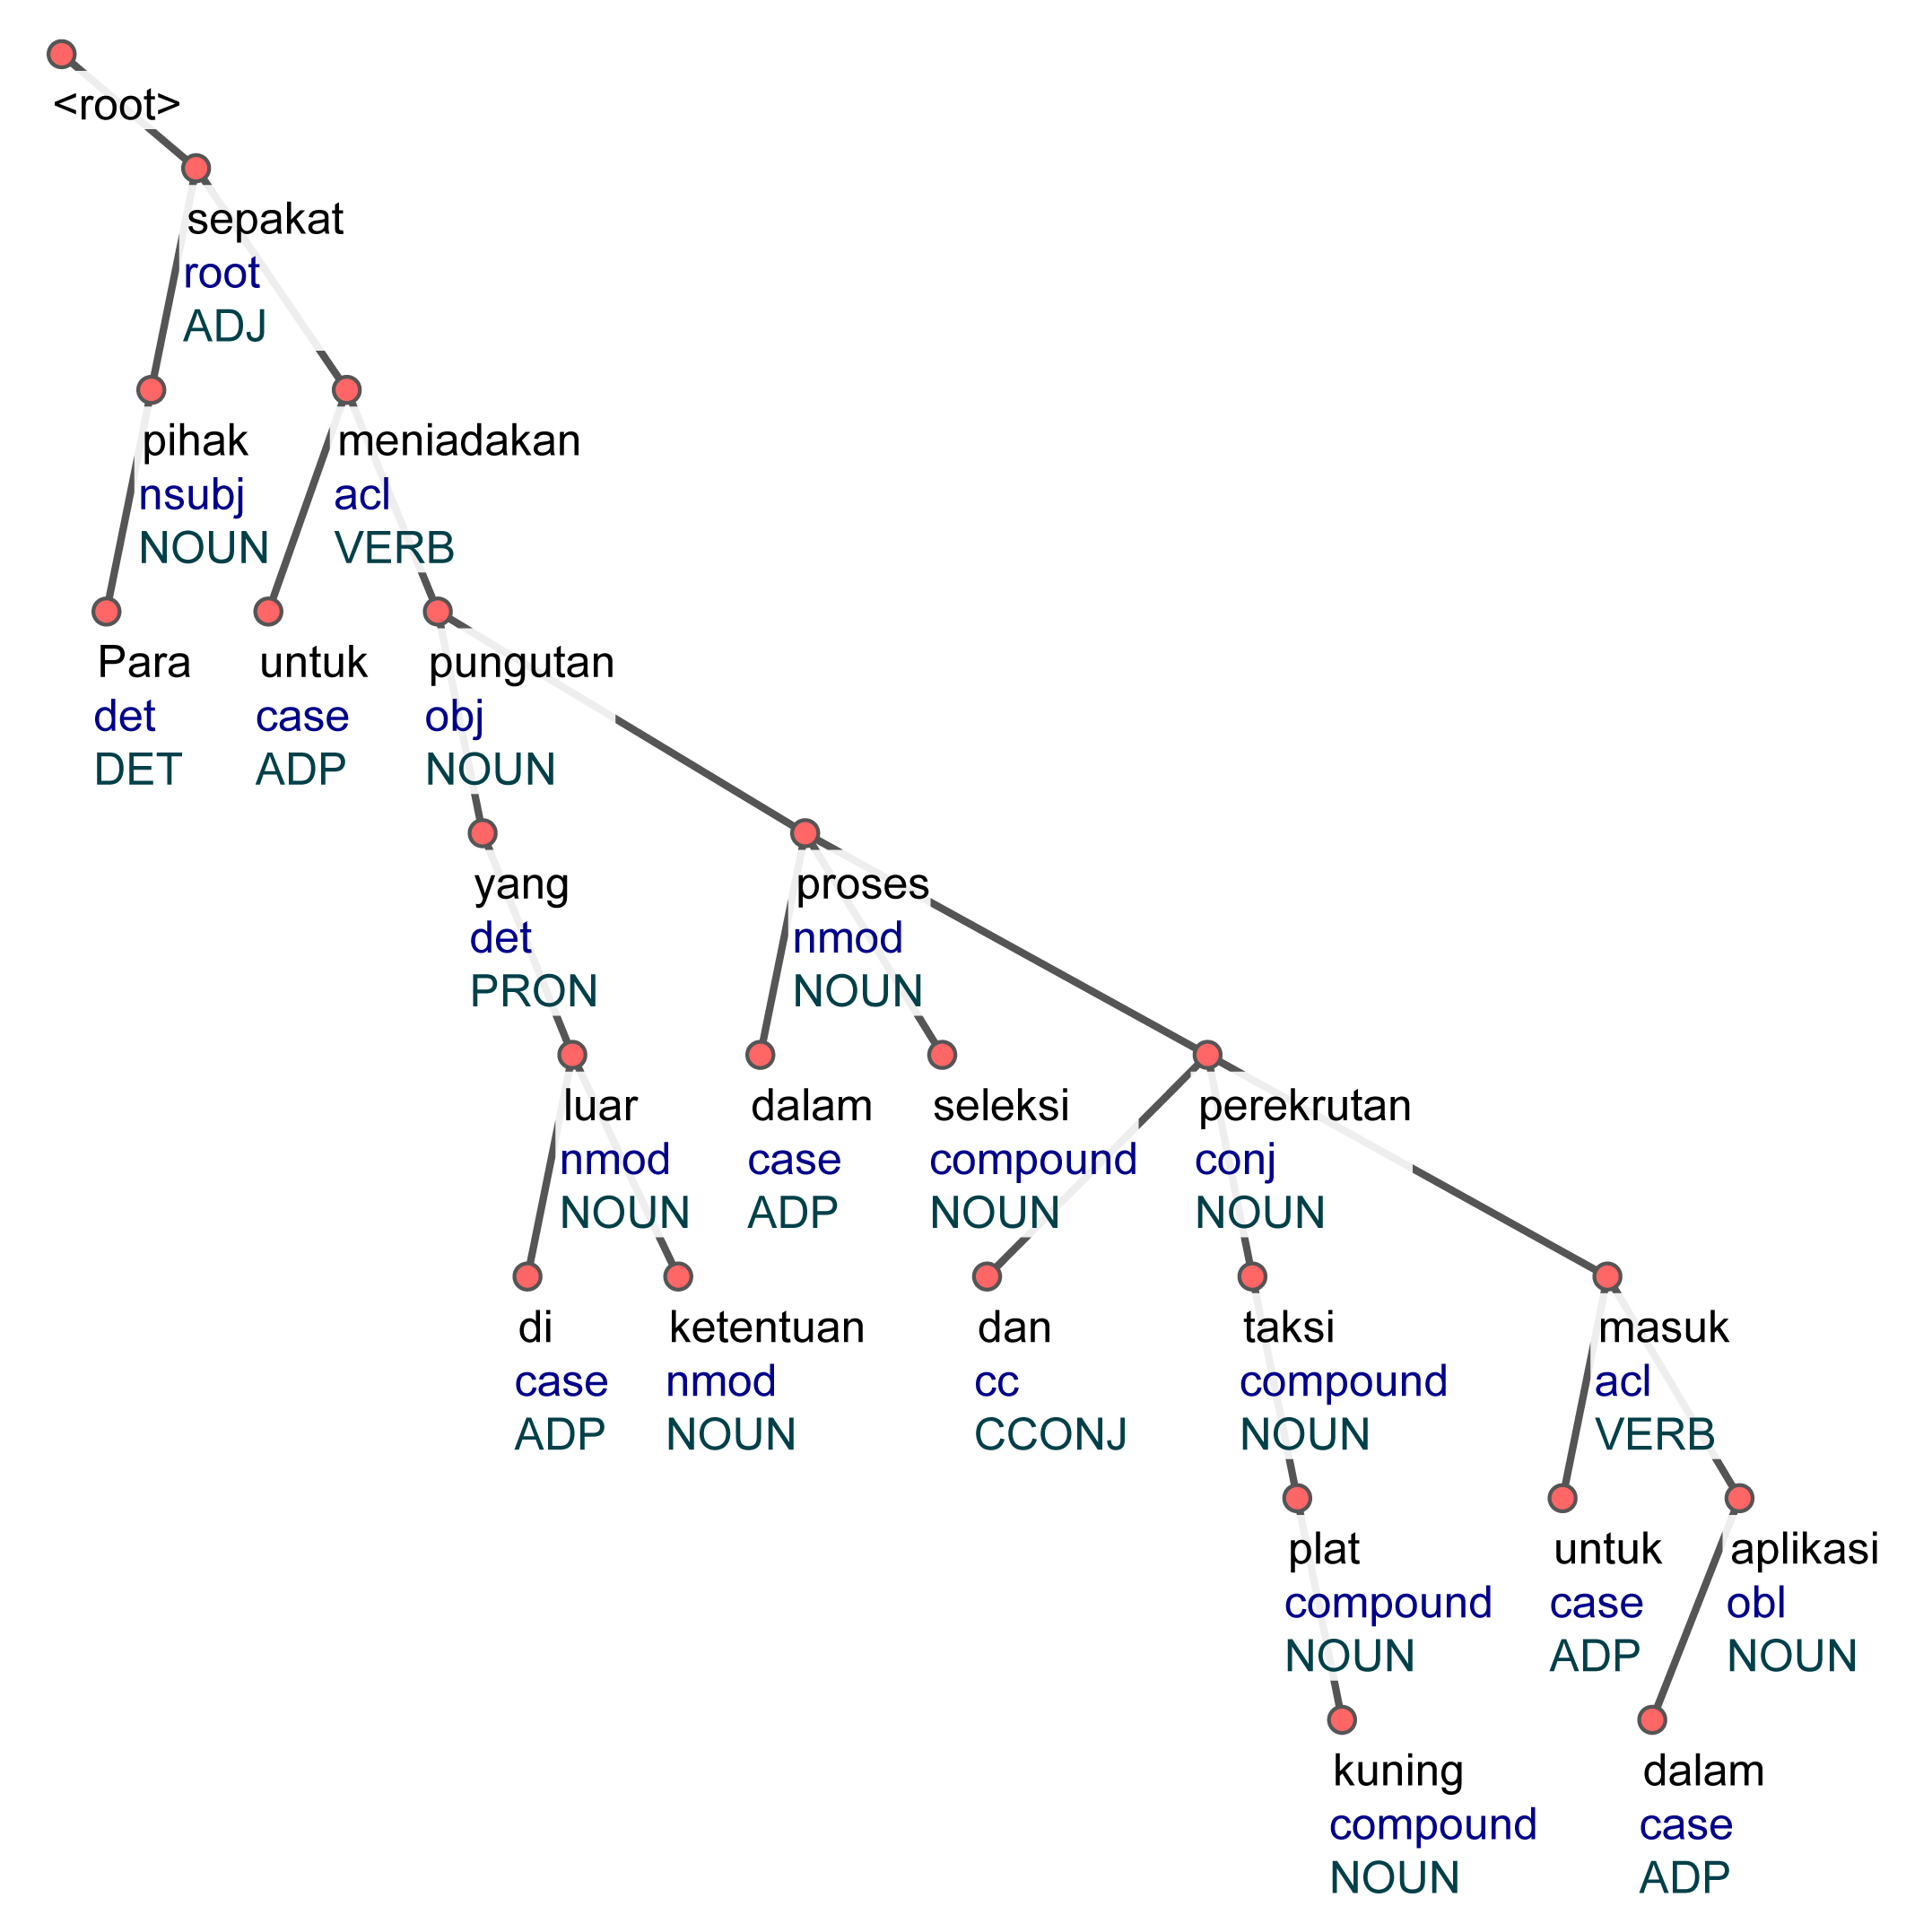
\includegraphics[width=0.8
	\textwidth] {pics/ts3901.jpg} 
	\caption{Kalimat T22 pada data ragam tulis} 
	\label{fig:ts3901} 
\end{figure}

Konstituen \textit{sepakat} pada kalimat T22 (\pic~\ref{fig:ts3901}) merupakan akar yang memiliki tautan-tautan dependensi terhadap konstituen-konstituen terikatnya. Induk pada simpai cabang terdekat pada kalimat T22 cenderung memiliki jumlah konstituen sedikit meskipun mengandung beberapa klausa terikat. Pada kalimat T22 ini terlihat banyak tautan dependensi dari dua konstituen yang berdampingan seperti pada relasi simpai-simpai antara konstituen \textit{para}, \textit{pihak}, dan \textit{sepakat}, antara konstituen \textit{meniadakan}, \textit{pungutan}, dan \textit{yang}, serta beberapa tautan lainnya. Berdasarkan bank pohon struktur dependensi ini, terlihat juga ada percabangan utama yang bersifat berlanjut antara \textit{sepakat}, \textit{meniadakan}, \textit{pungutan}, \textit{proses}, \textit{perekrutan}, dan \textit{masuk}. Relasi berlanjut ini mencerminkan adanya percabangan searah meskipun bukan terhadap dua konstituen yang berdampingan. Kalimat T22 (\pic~\ref{fig:ts3901}) memiliki DL sejauh 35 dan MDD sejauh 1,667 konstituen. Selisih antara DL dari tautan-tautan dependensi positif dan negatif sebesar 19 dalam arti jumlah tautan dengan bentuk relasi diawali induk lebih banyak dan/atau berjarak lebih jauh dibandingkan bentuk relasi yang sebaliknya.


\begin{figure}
	\centering 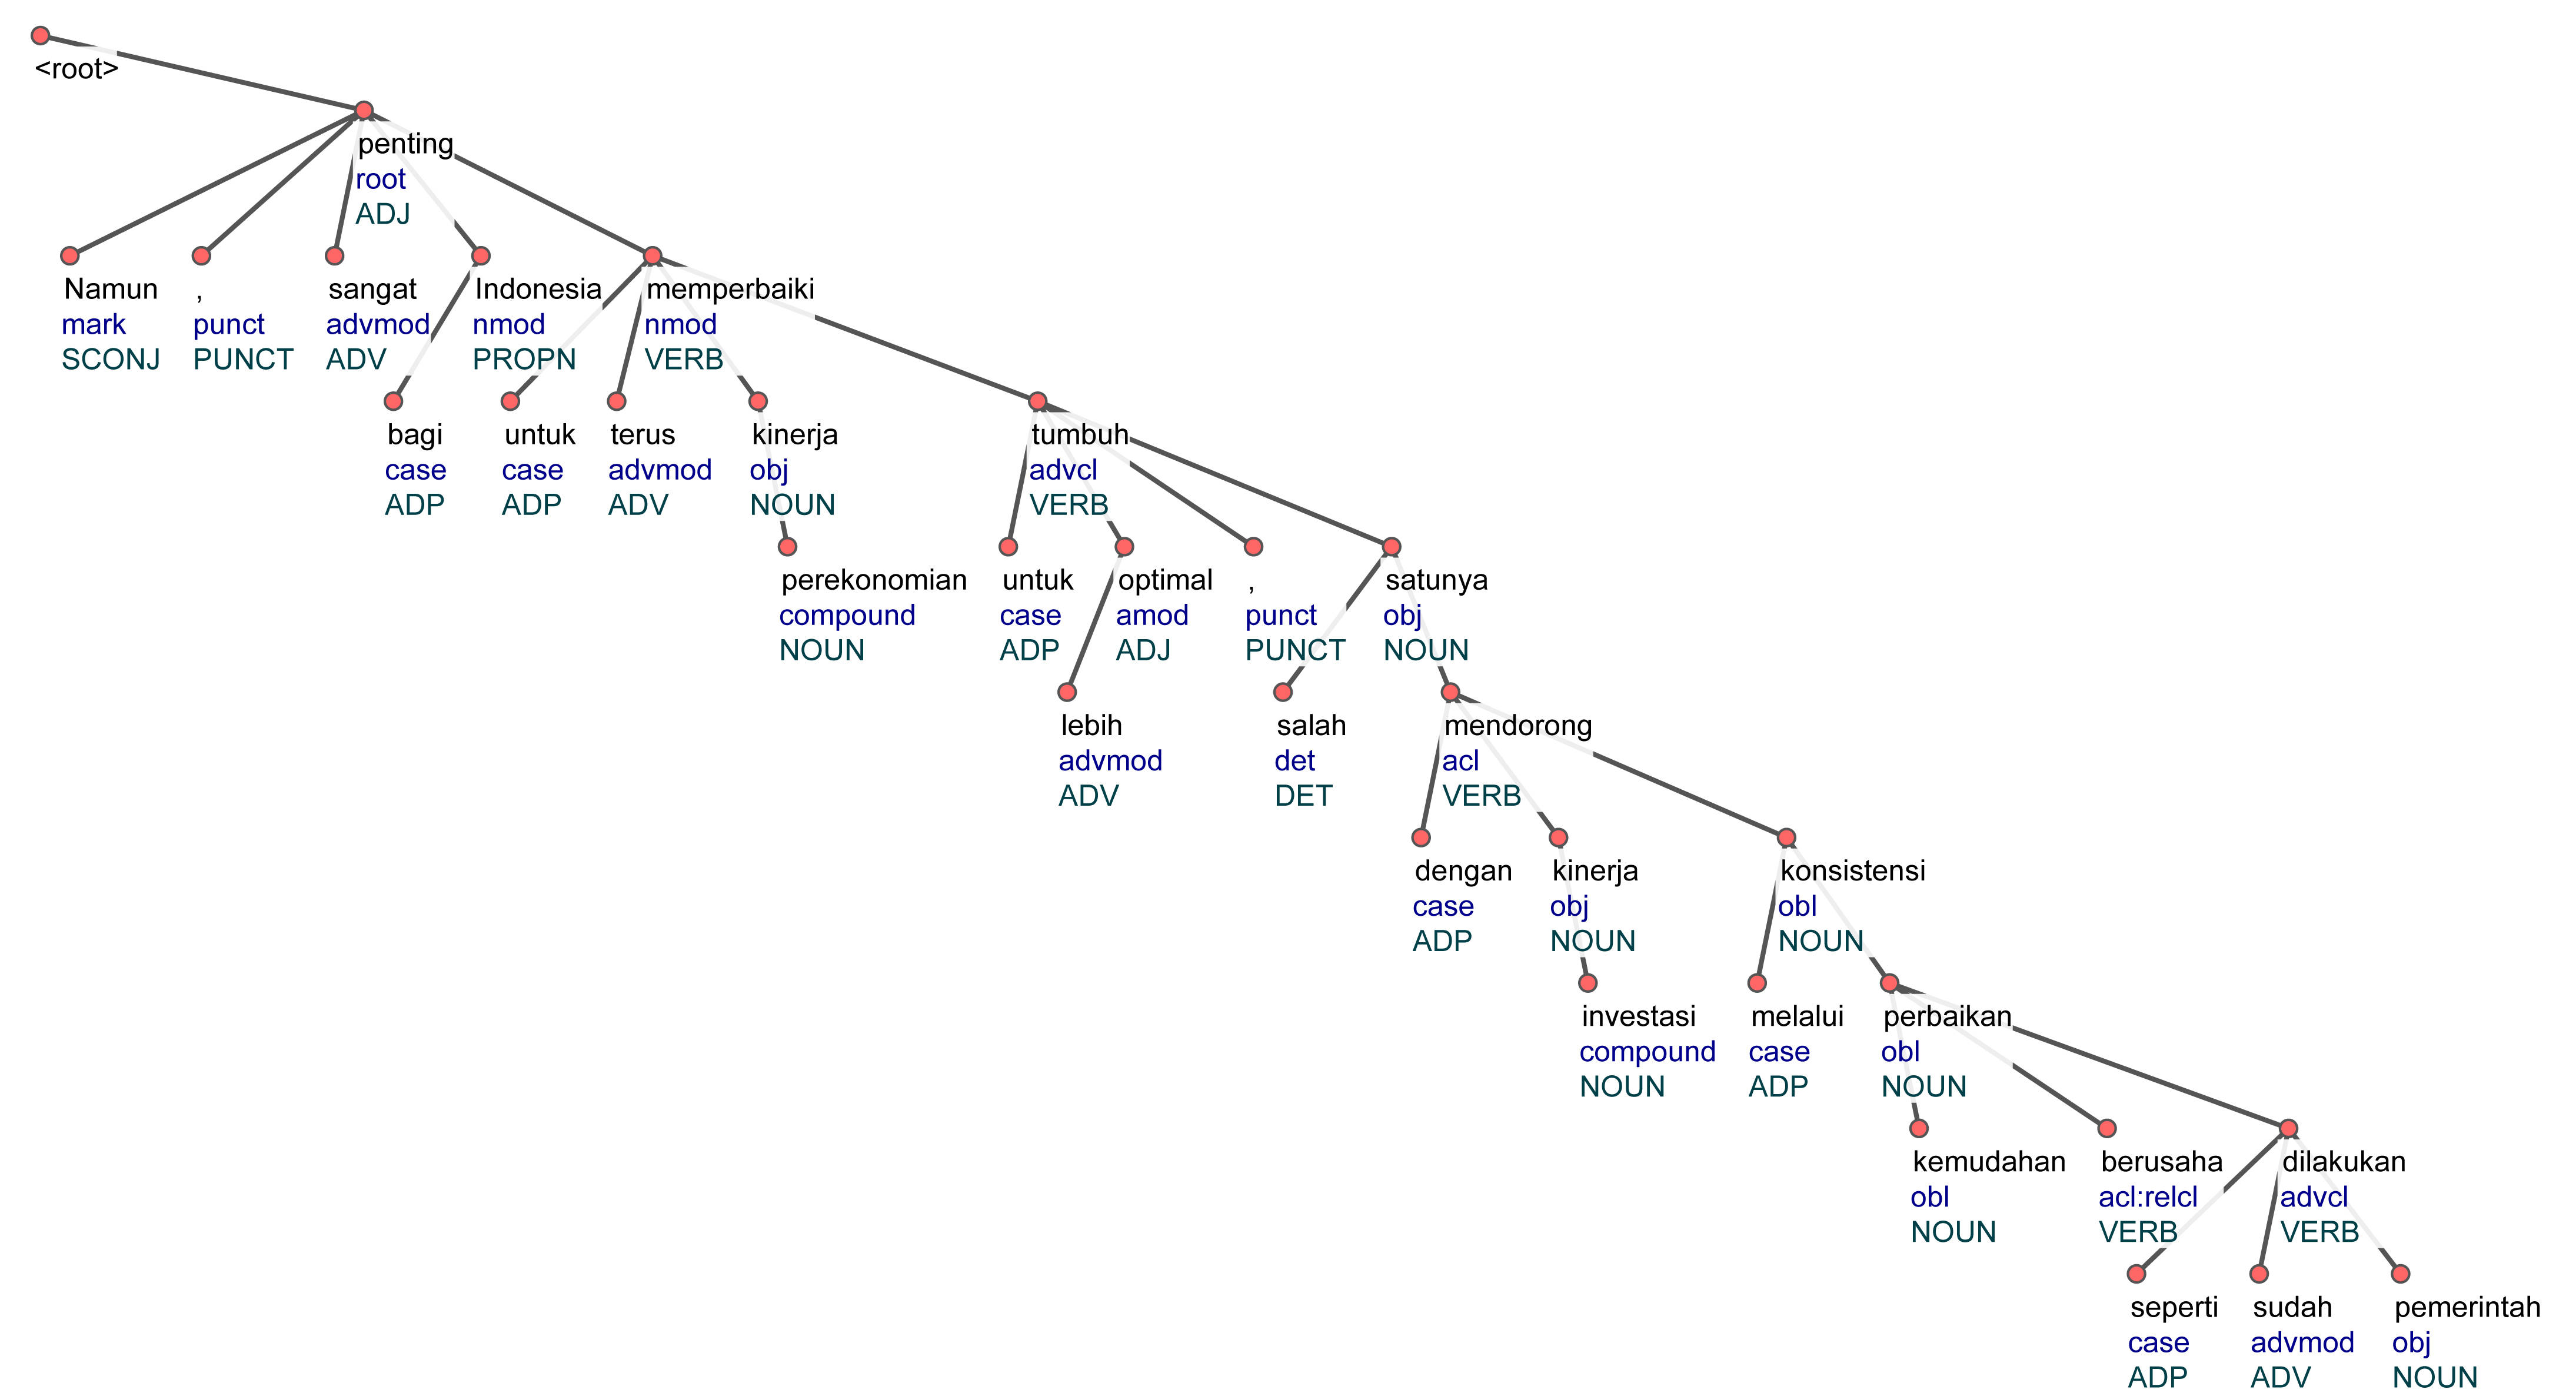
\includegraphics[width=1
	\textwidth] {pics/ts2079.jpg} 
	\caption{Kalimat T31a pada data ragam tulis} 
	\label{fig:ts2079} 
\end{figure}

Akar adjektiva \textit{penting} pada kalimat T31a (\pic~\ref{fig:ts2079}) mengikat verba \textit{memperbaiki} yang dihubungkan dengan konjungsi \textit{untuk} dalam kaidah dependensi. Induk pada simpai cabang terdekat ini juga cenderung memiliki jumlah konstituen sedikit meskipun mengandung beberapa klausa terikat. Pola ini terlihat berulang pada simpai-simpai cabang berikutnya mengakibatkan banyak simpai cabang lain yang tidak memiliki tautan langsung dengan akar dan banyak terbentuk tautan antara dua konstituen yang berdampingan. Seperti kalimat T22, relasi antara simpai-simpai konstituen \textit{penting}, \textit{memperbaiki}, \textit{kinerja}, \textit{mendorong}, \textit{konsistensi}, \textit{berusaha}, dan \textit{dilakukan} bersifat berlanjut mencerminkan adanya percabangan searah meskipun bukan terhadap dua konstituen yang berdampingan. Kalimat T31a (\pic~\ref{fig:ts2079}) memiliki DL sejauh 68 dan MDD sejauh 2,267 konstituen. Selisih antara DL dari tautan-tautan dependensi positif dan negatif sebesar 16 yang juga berarti jumlah tautan dengan bentuk relasi diawali induk lebih banyak dan/atau berjarak lebih jauh dibandingkan bentuk relasi yang sebaliknya.

\begin{figure}
	\centering 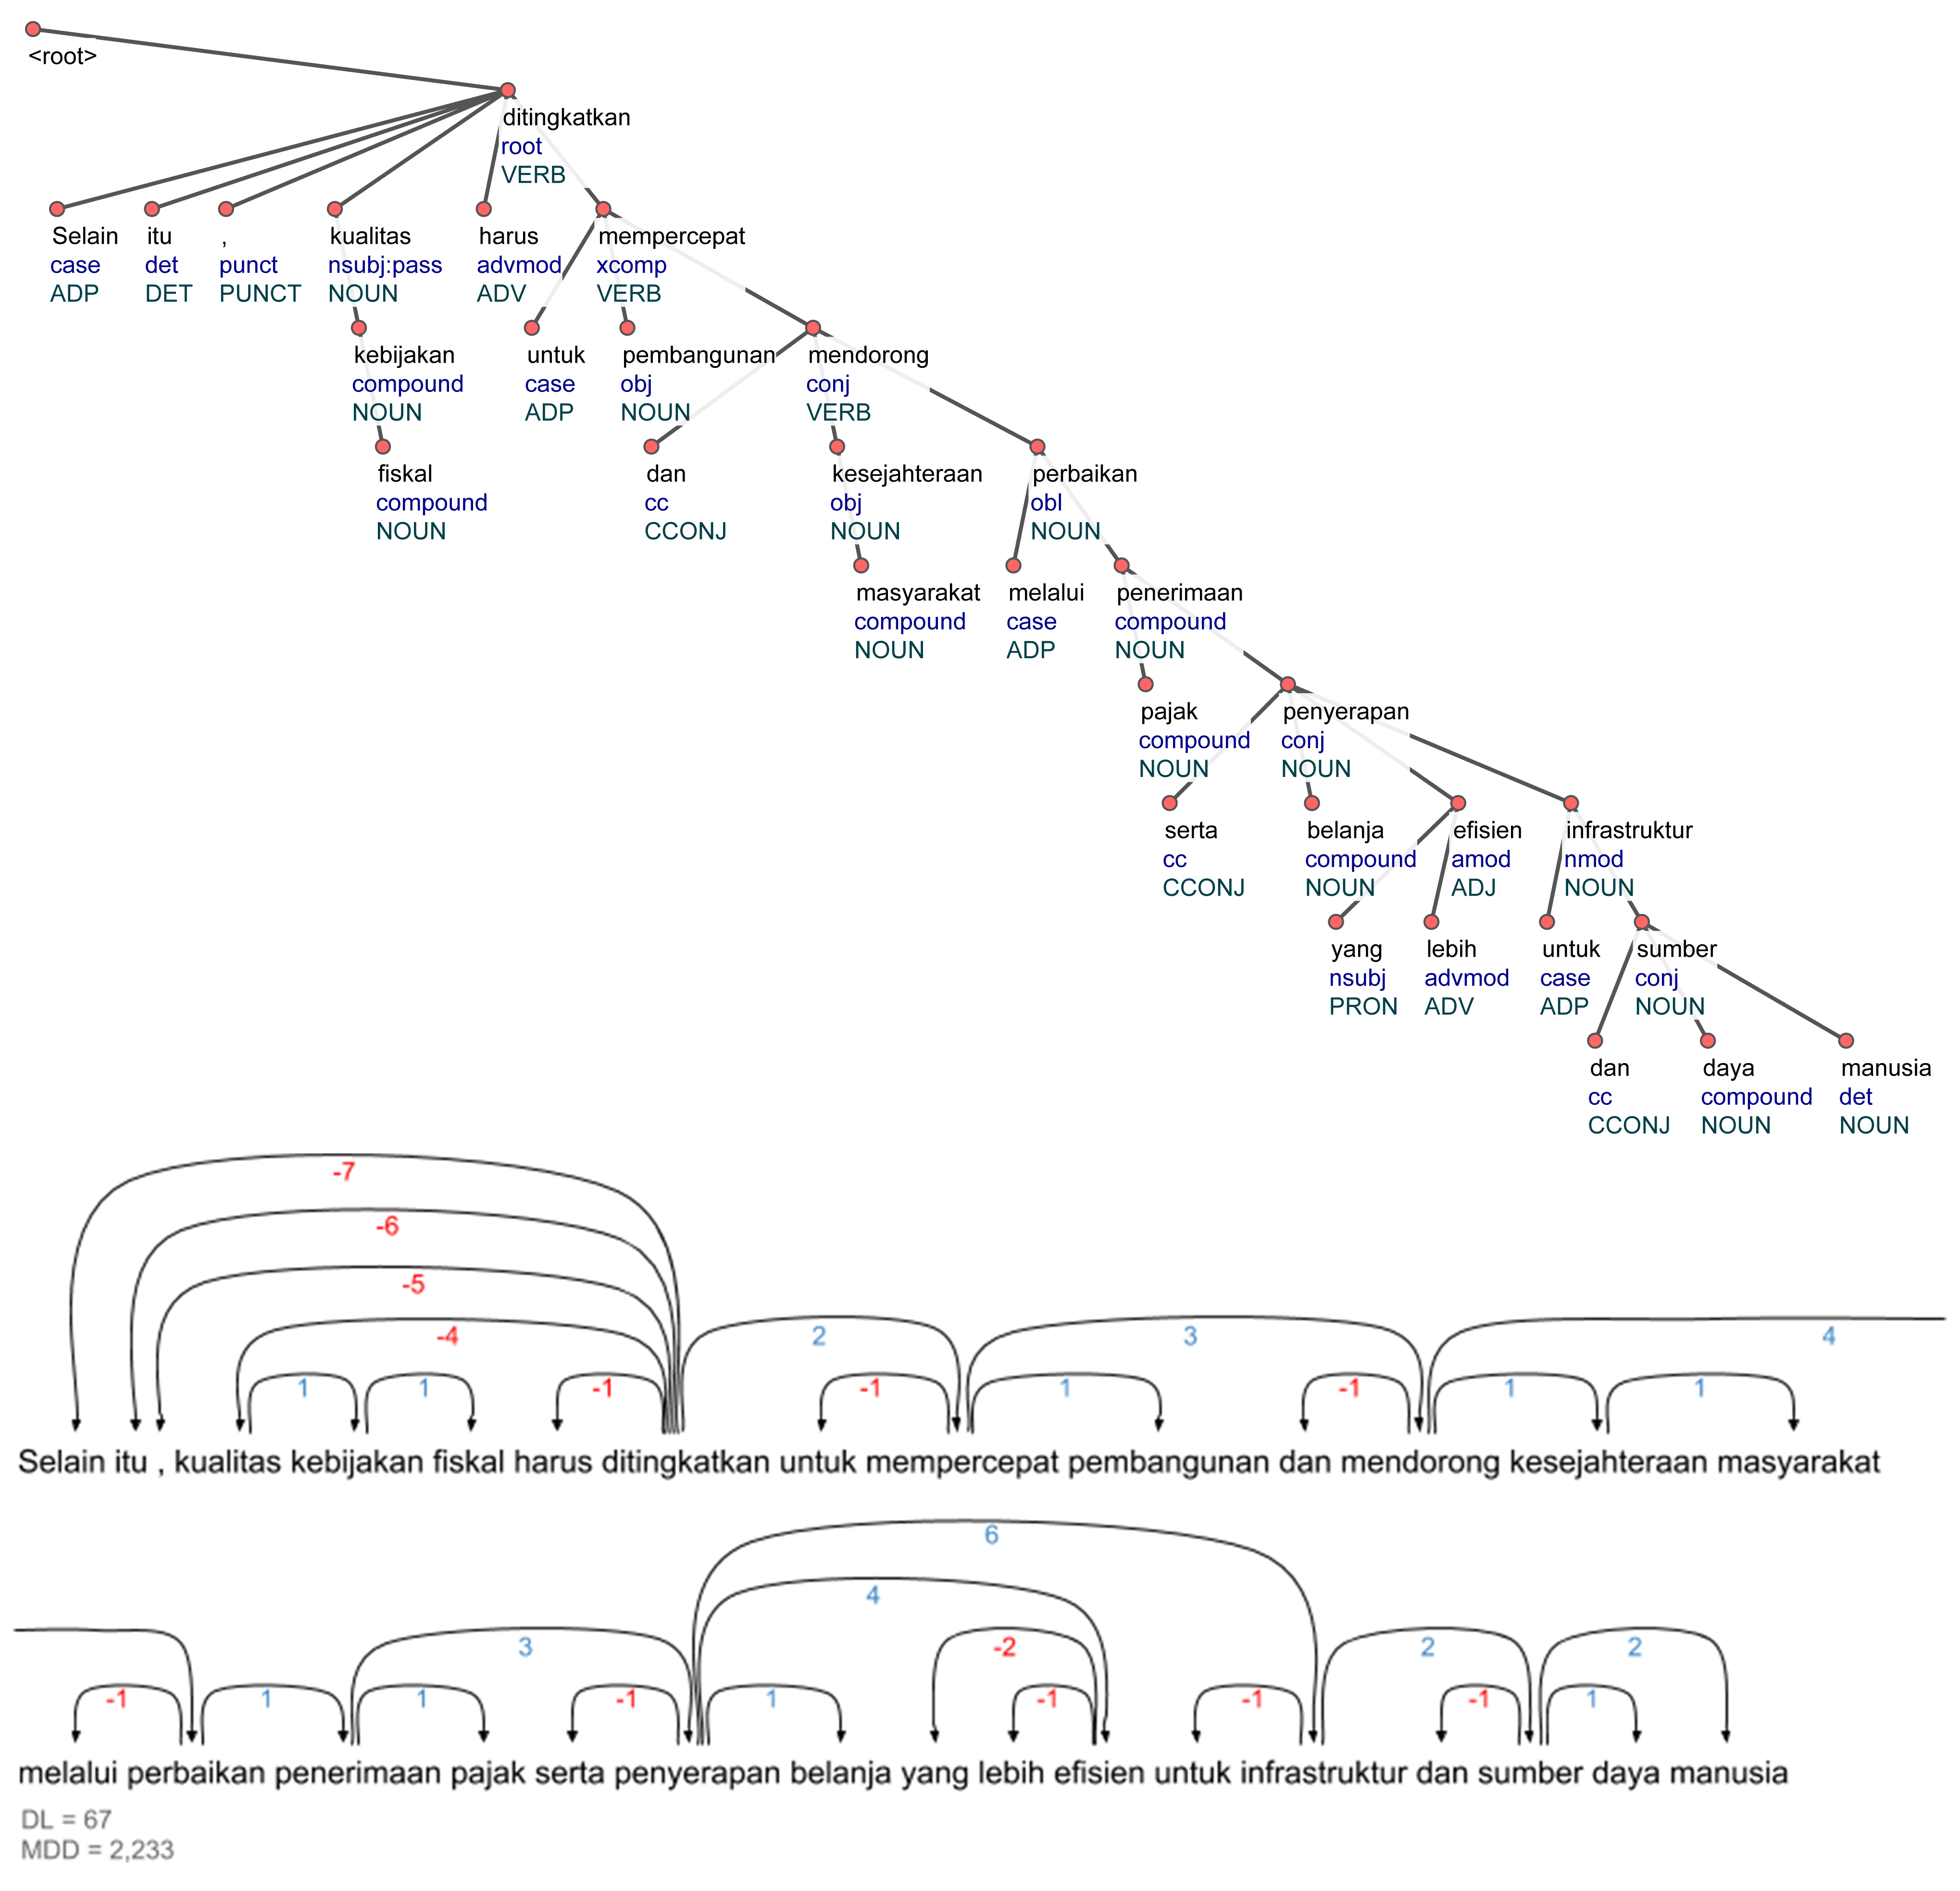
\includegraphics[width=1
	\textwidth] {pics/ts2081.jpg} 
	\caption{Kalimat T31b pada data ragam tulis} 
	\label{fig:ts2081} 
\end{figure}

Seperti kalimat T22 dan T31a, konstituen \textit{ditingkatkan} pada kalimat T31b (\pic~\ref{fig:ts2081}) juga merupakan akar yang memiliki beberapa tautan dependensi terhadap konstituen terikatnya. Pada kalimat ini, akar verbal \textit{ditingkatkan} mengikat verba lain \textit{mempercepat} yang juga dihubungkan dengan konjungsi tujuan \textit{untuk}. Juga seperti kalimat T31a, banyak simpai-simpai cabang pada kalimat T31b tidak memiliki tautan langsung dengan akar mengakibatkan adanya percabangan searah. Kalimat T31b (\pic~\ref{fig:ts2081}) memiliki DL sejauh 67 dan MDD sejauh 2,233 konstituen. Meskipun struktur kalimat T31b terlihat serupa dengan kalimat T31a dan DL serta MDD yang cukup dekat, selisih DL dari tautan-tautan dependensi positif dan negatif sangat kecil, yaitu hanya sebesar 3. Hal ini berarti jumlah bentuk relasi diawali induk dan jumlah bentuk relasi diakhiri induk dalam kalimat tersebut cukup seimbang. 

Pada ketiga kalimat, terutama kalimat T22 dan T31a, terlihat pergerakan simpai dan percabangan yang semakin menurun ke arah sesudah akar atau ke arah kanan. Percabangan menurun ke kanan ini juga menunjukkan indikasi adanya strategi untuk menghasilkan dependensi positif atau bentuk relasi antarkonstituen utama yang diawali induk. Struktur kalimat dengan karakteristik seperti pada \pic~\ref{fig:ts3901}, \pic~\ref{fig:ts2079} dan \pic~\ref{fig:ts2081} ini cukup umum dalam korpus data ragam tulis klasifikasi kalimat panjang. Namun, seperti yang terlihat pada perbandingan selisih DL antara kalimat T31a dan T31b, dominasi percabangan searah pada kalimat T31a tidak selalu menghasilkan panjang dan jarak dependensi yang lebih pendek dibandingkan kalimat T31b yang memiliki keseimbangan antara kedua bentuk relasi induk dan konstituen terikat. Hal ini mungkin disebabkan karena kalimat T31b memiliki jumlah tautan dependensi antara dua konstituen yang berdampingan lebih banyak dibandingkan T31a.

\begin{figure}
	\centering 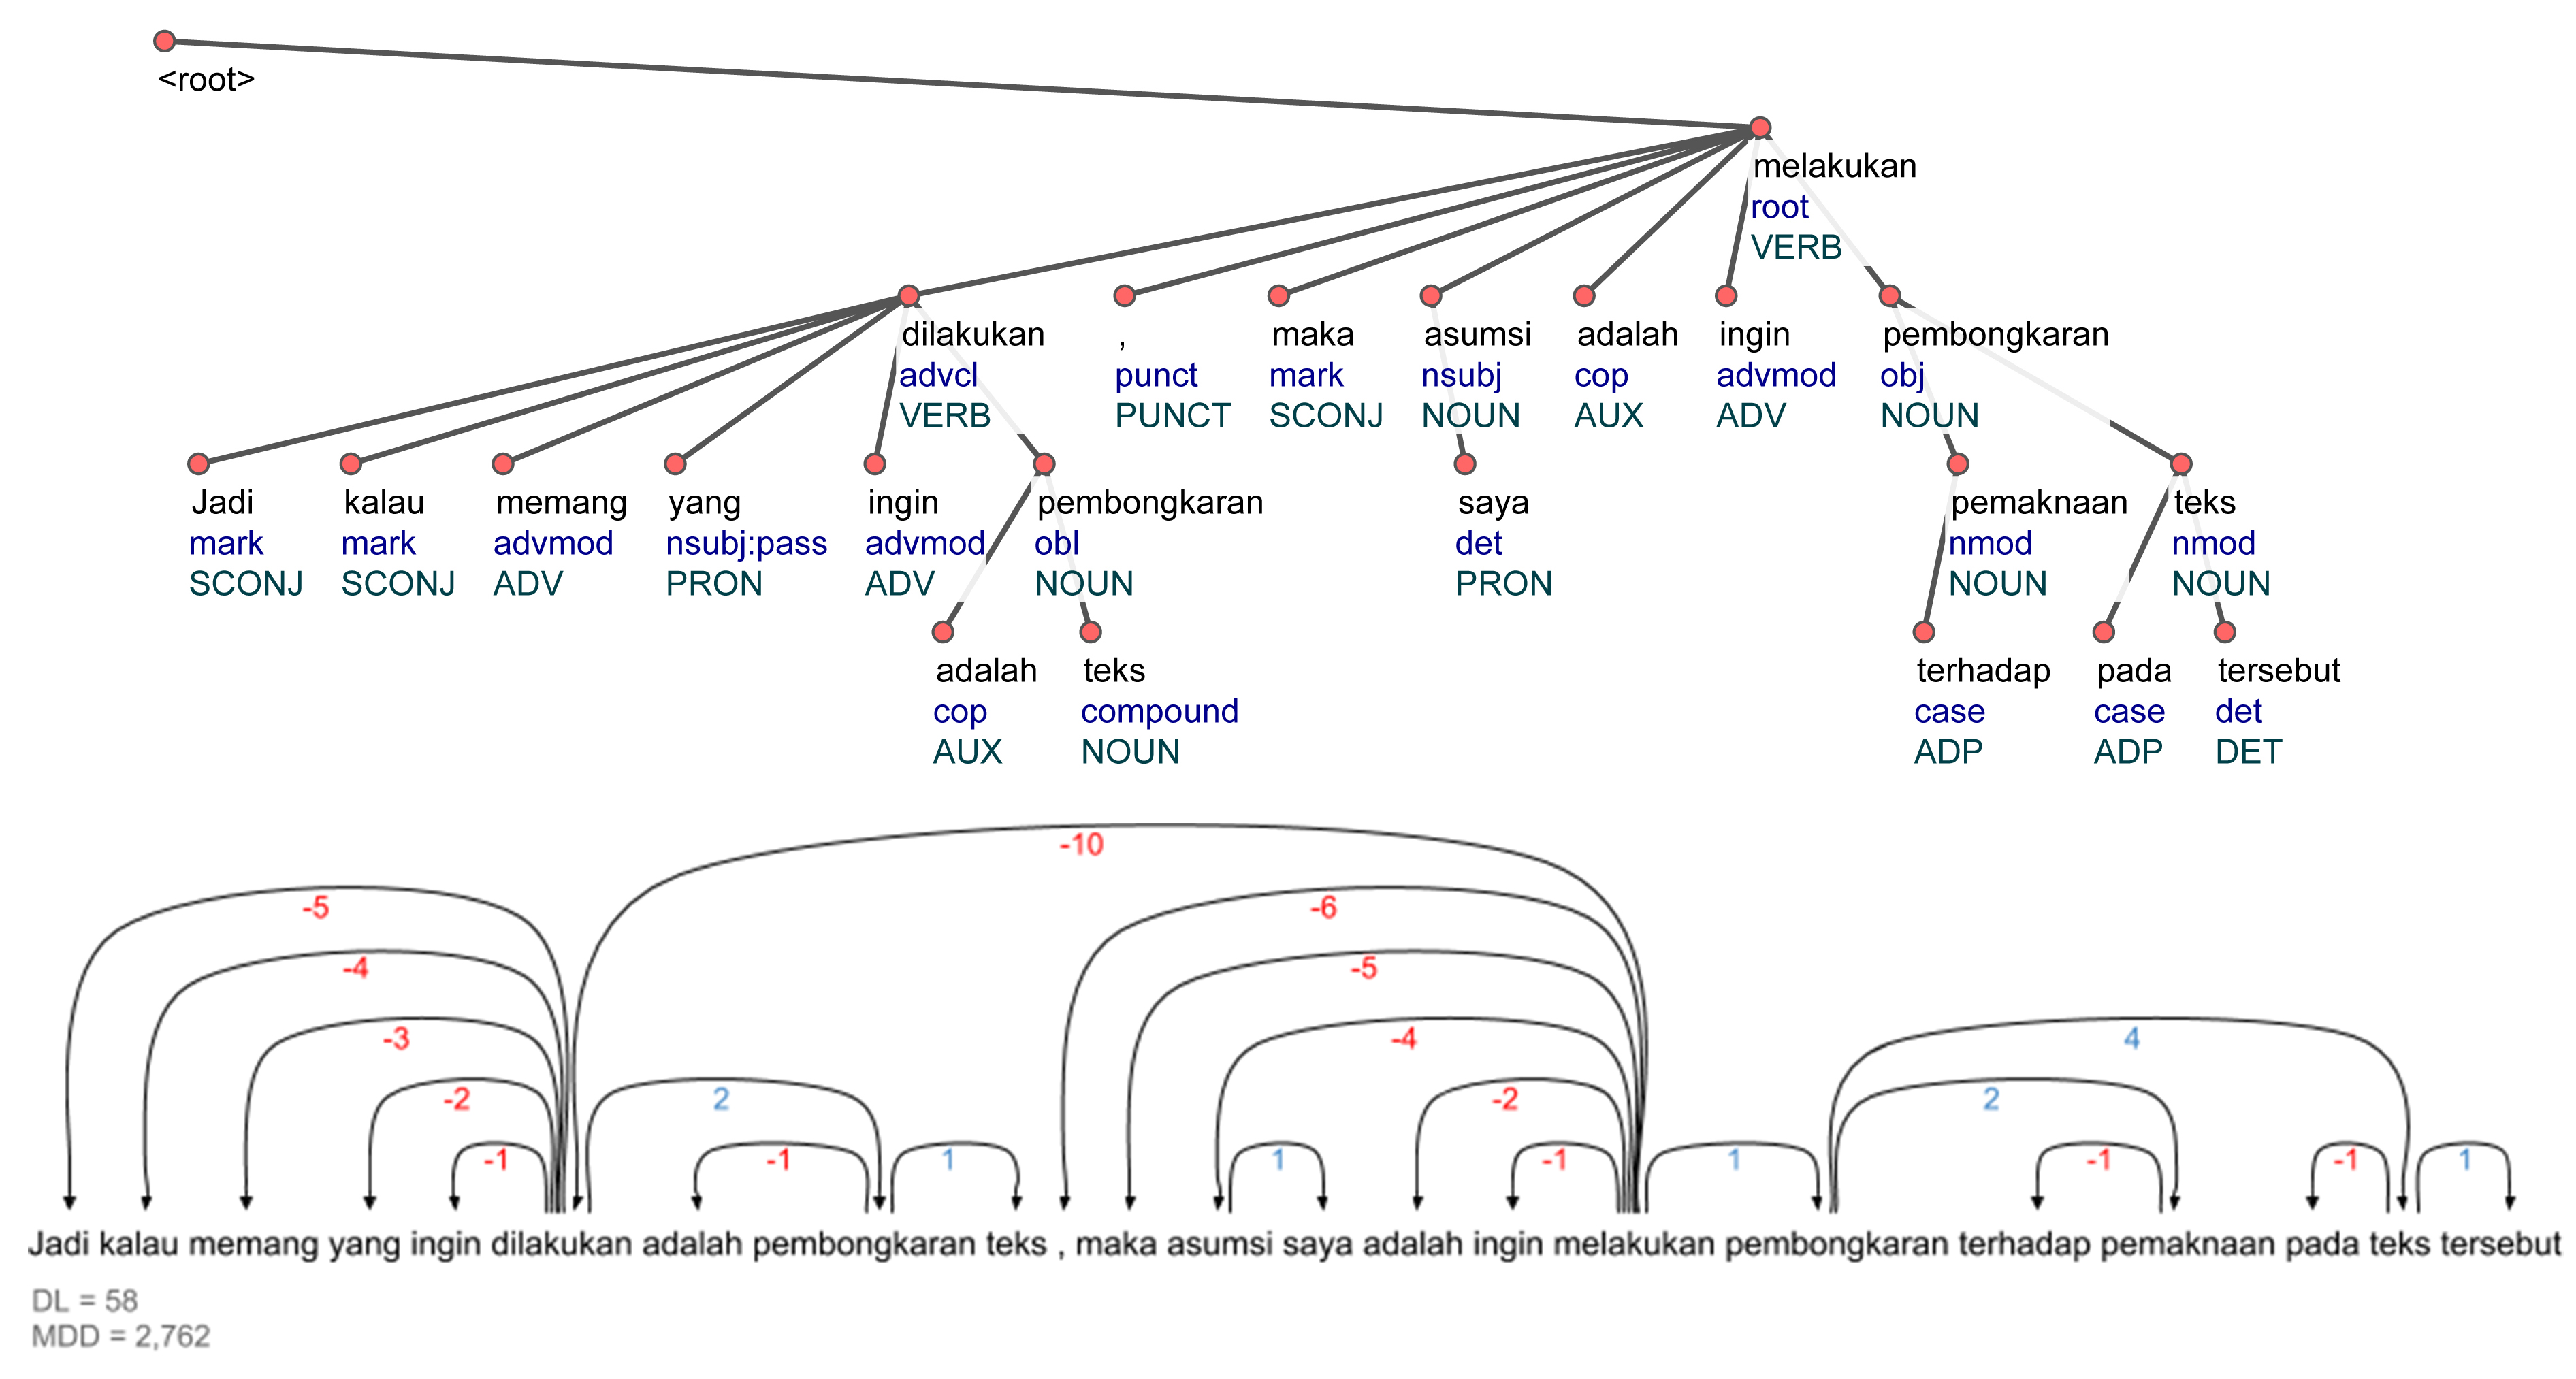
\includegraphics[width=1
	\textwidth] {pics/ls6521.jpg} 
	\caption{Kalimat L22 pada data ragam lisan} 
	\label{fig:ls6521} 
\end{figure}

Kalimat L22 (\pic~\ref{fig:ls6521}) memiliki akar verba \textit{melakukan} dan mengikat banyak konsituen terikat. Pada kalimat ini, terlihat bagaimana tautan dependensi dan percabangan jauh lebih menyebar dibandingkan dengan contoh-contoh kalimat dalam ragam tulis. Percabangan yang menyebar ini menyebabkan tautan-tautan dependensi berjarak jauh karena tautan dependensi antara dua konstituen yang berdampingan jumlahnya lebih sedikit dibandingkan dengan contoh-contoh pada ragam tulis. Dua percabangan utama terlihat pada simpai \textit{dilakukan} dan simpai pusat \textit{melakukan}. Penyebaran simpai-simpai ini juga berakibat pada tingkat kedalaman dependensi yang lebih dangkal dibandingkan dengan contoh-contoh pada ragam tulis. Akar \textit{melakukan} juga tidak memiliki aktor pelaku seperti pada contoh kalimat L4 (pic~\ref{fig:ls1102}). Pada kedua kasus ini, aktor pelaku terhadap verba-verba tersebut mungkin baru akan dimengerti dengan memahami relasi pada tataran diskursus. Kalimat L22 ini memiliki DL sejauh 57 dan MDD sejauh 2,714 konstituen. 

\begin{figure}
	\centering 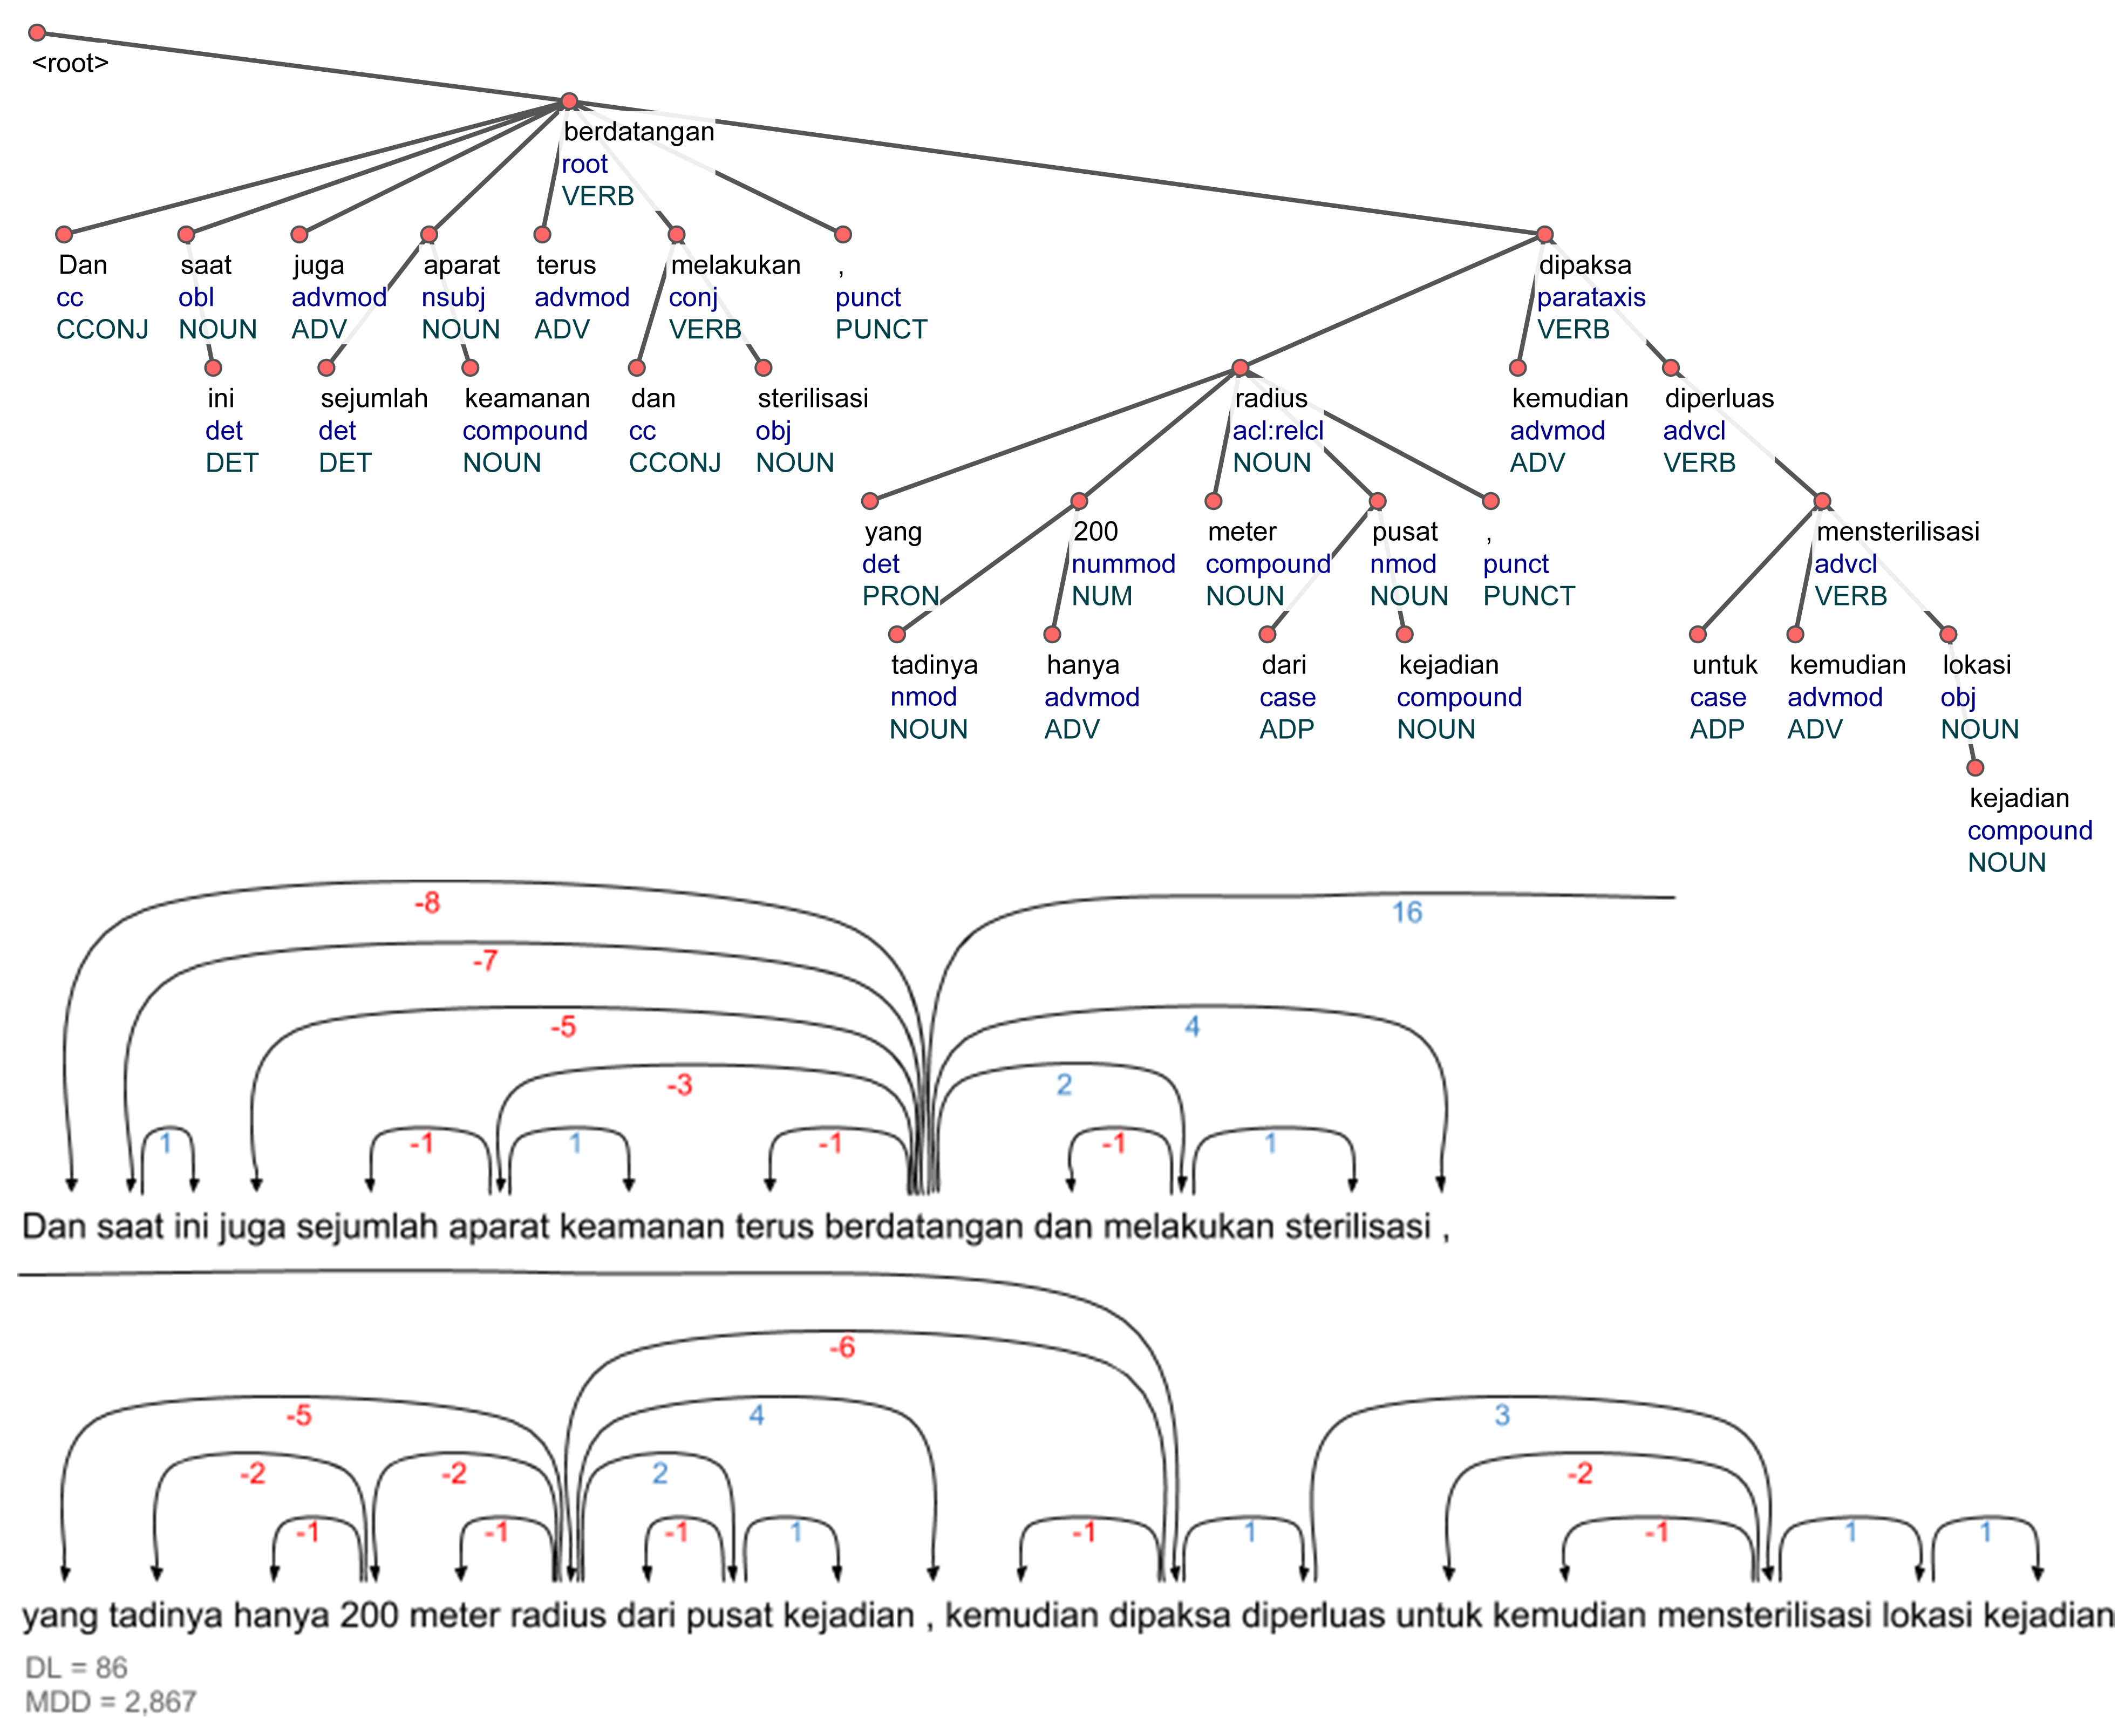
\includegraphics[width=1
	\textwidth] {pics/ls1716.jpg} 
	\caption{Kalimat L31a pada data ragam lisan} 
	\label{fig:ls1716} 
\end{figure}

Pada kalimat L31a (\pic~\ref{fig:ls1716}), simpai pusat dan simpai cabang pada verba \textit{dipaksa} memiliki banyak tautan yang juga cukup menyebar dibandingkan dengan contoh kalimat pada ragam tulis. Kalimat ini memperlihatkan adanya pembagian informasi secara besar seperti pada kalimat L22. Relasi akar verbal \textit{berdatangan} dengan verba \textit{dipaksa} memiliki tipe dependensi $parataxis$. Tipe ini menandakan relasi yang menyerupai koordinasi antar diskursus, dalam arti seluruh informasi yang dibawa oleh simpai konstituen terikat ini memiliki kualitas kalimat utuh sehingga bisa menjadi kalimat terpisah. Kalimat L31a (\pic~\ref{fig:ls1716}) memiliki DL sejauh 86 dan MDD sejauh 2,867 konstituen. 

\begin{figure}
	\centering 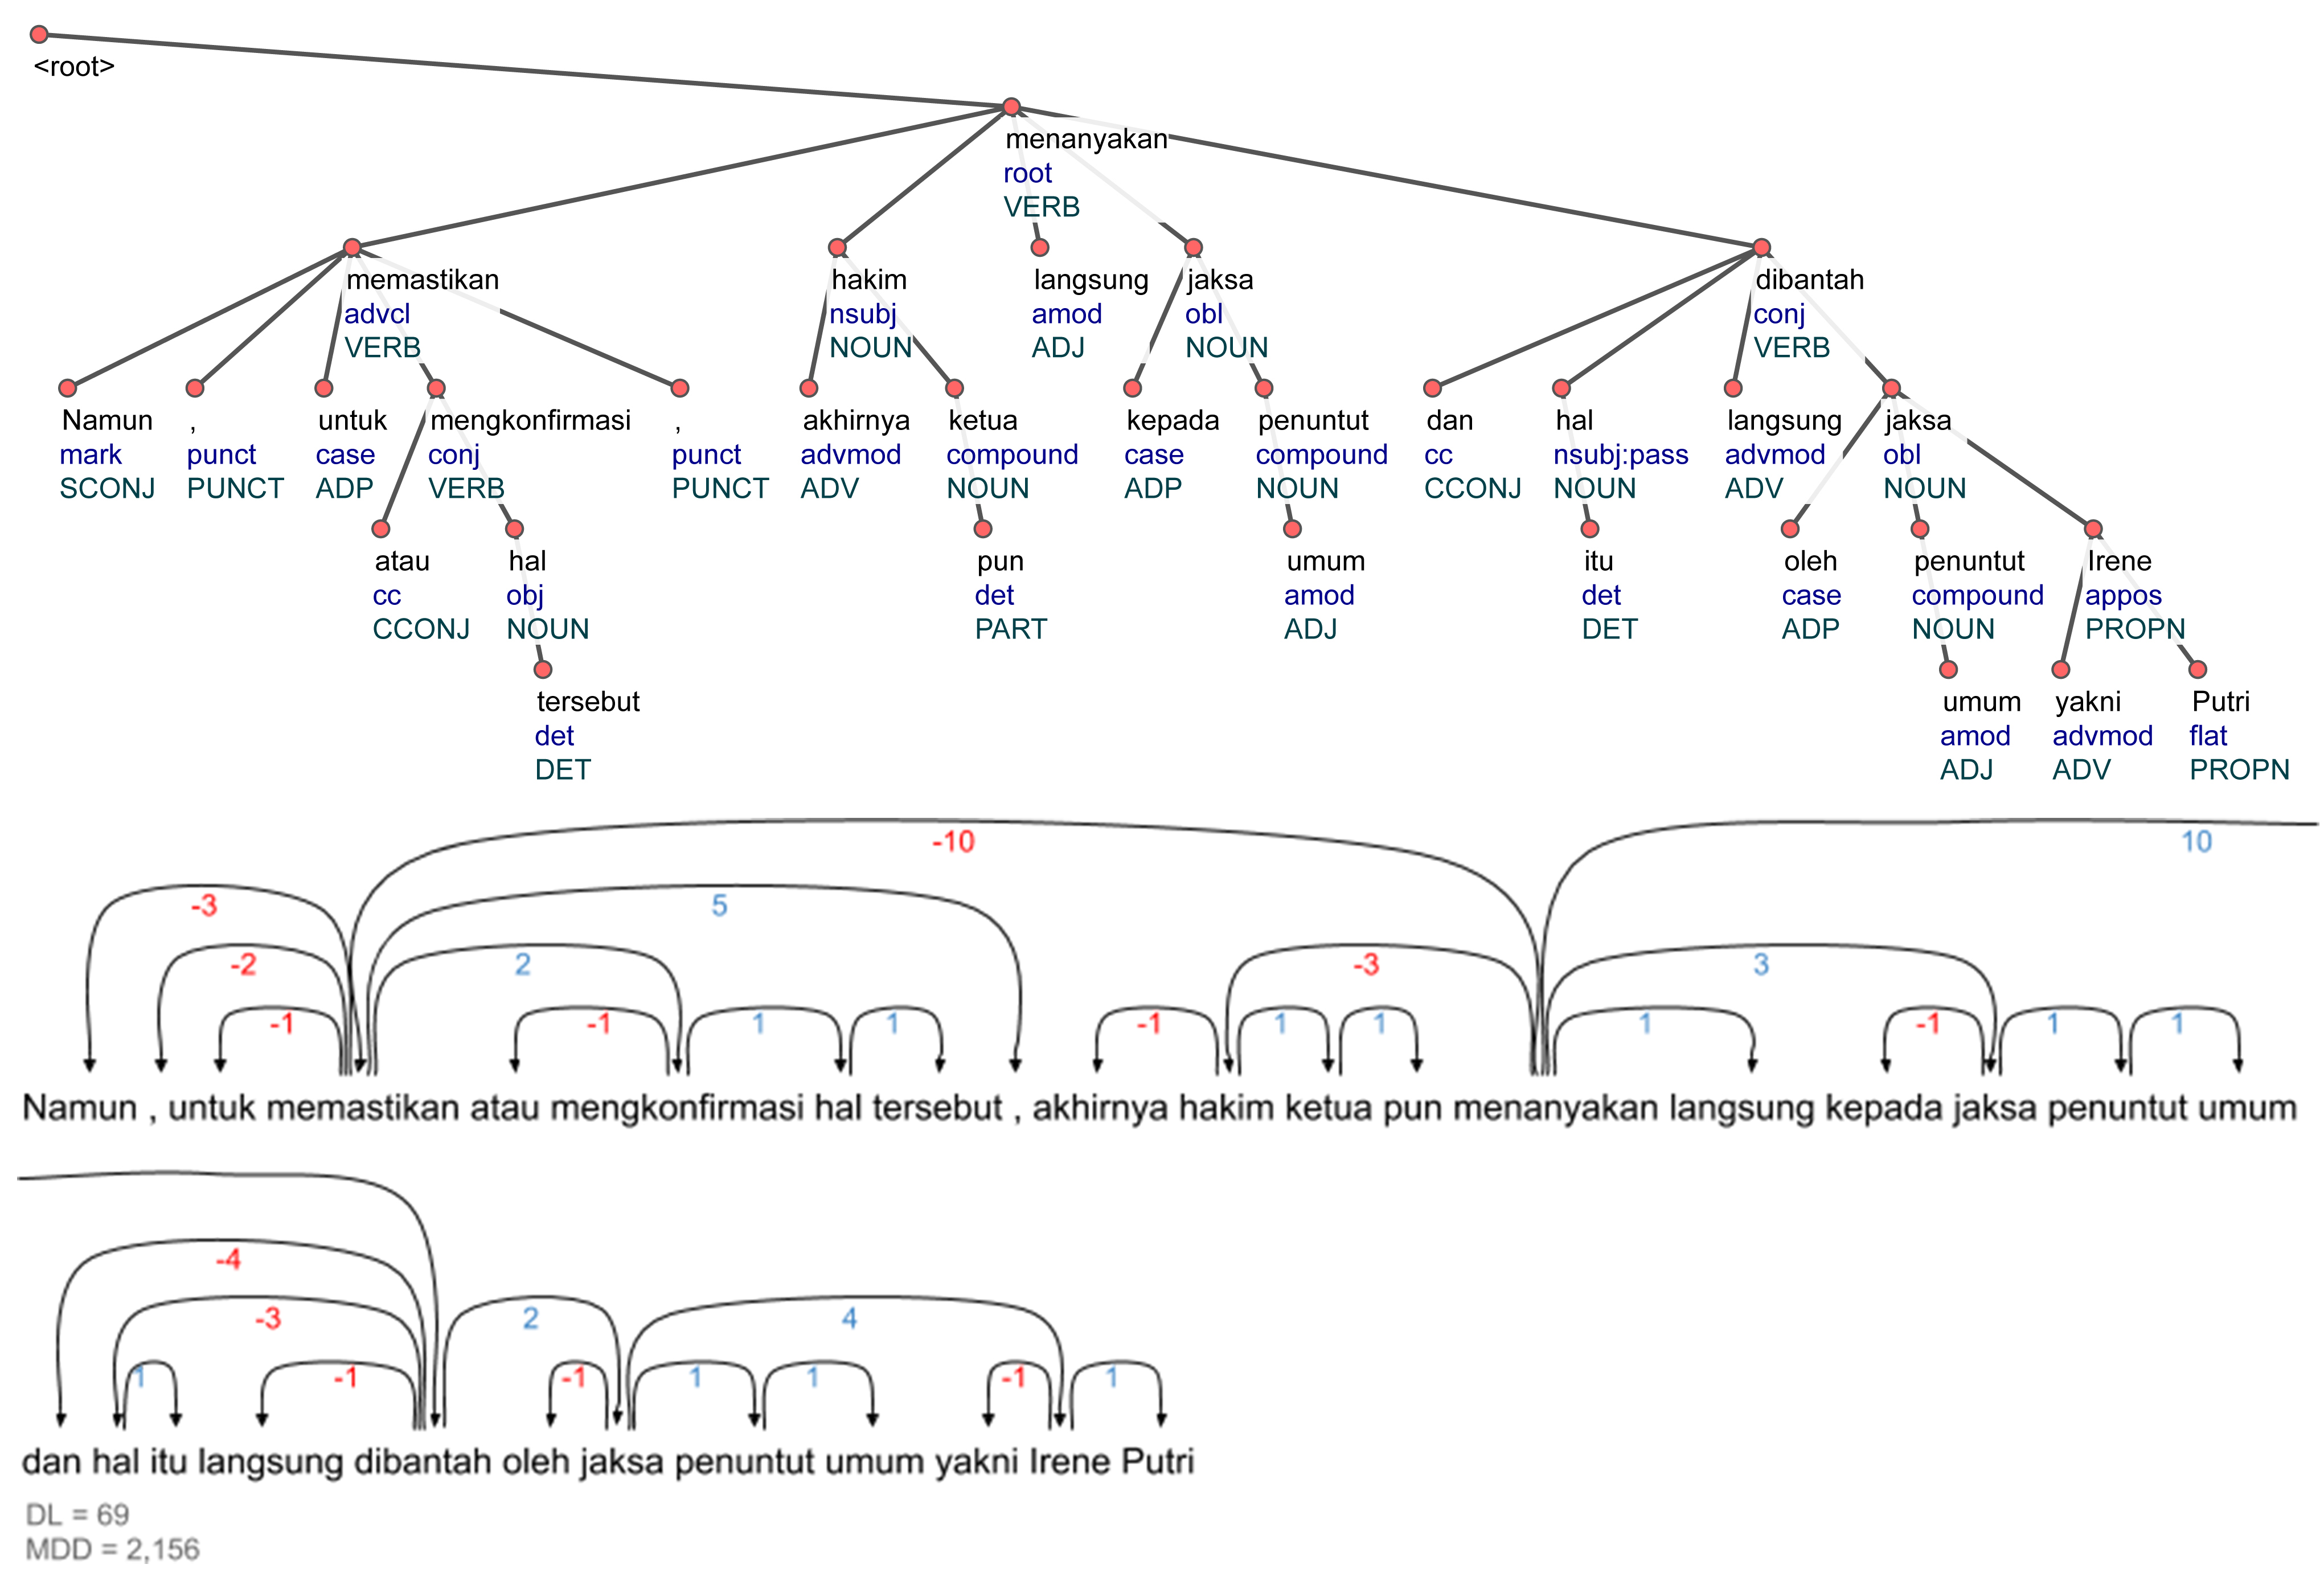
\includegraphics[width=1
	\textwidth] {pics/ls16.jpg} 
	\caption{Kalimat L31b pada data ragam lisan}
	\label{fig:ls16} 
\end{figure}

Pada kalimat L31b (\pic~\ref{fig:ls16}), posisi akar berada di tengah kalimat. Seluruh informasi yang dibawa klausa tujuan dengan induk \textit{memastikan} direalisasikan sebelum akar verbal \textit{menanyakan}. Akar verbal ini juga mengikat verba \textit{dibantah} yang dihubungkan dengan konjungsi \textit{dan}. Kalimat ini tidak memiliki kandungan informasi yang bersifat diskursus seperti kalimat L31b, namun jumlah simpai-simpai cabang di bawah \textit{memastikan}, \textit{menanyakan}, dan \textit{dibantah} juga tersebar cukup merata. Kalimat L31b (\pic~\ref{fig:ls16}) memiliki DL sejauh 67 dan MDD sejauh 2,233 konstituen. Seperti kalimat T31b, selisih DL dari tautan-tautan dependensi positif dan negatif sangat kecil (sebesar 3) sehingga juga menandakan jumlah bentuk relasi diawali induk dan jumlah bentuk relasi diakhiri induk yang cukup seimbang. 

\begin{figure}
	\centering 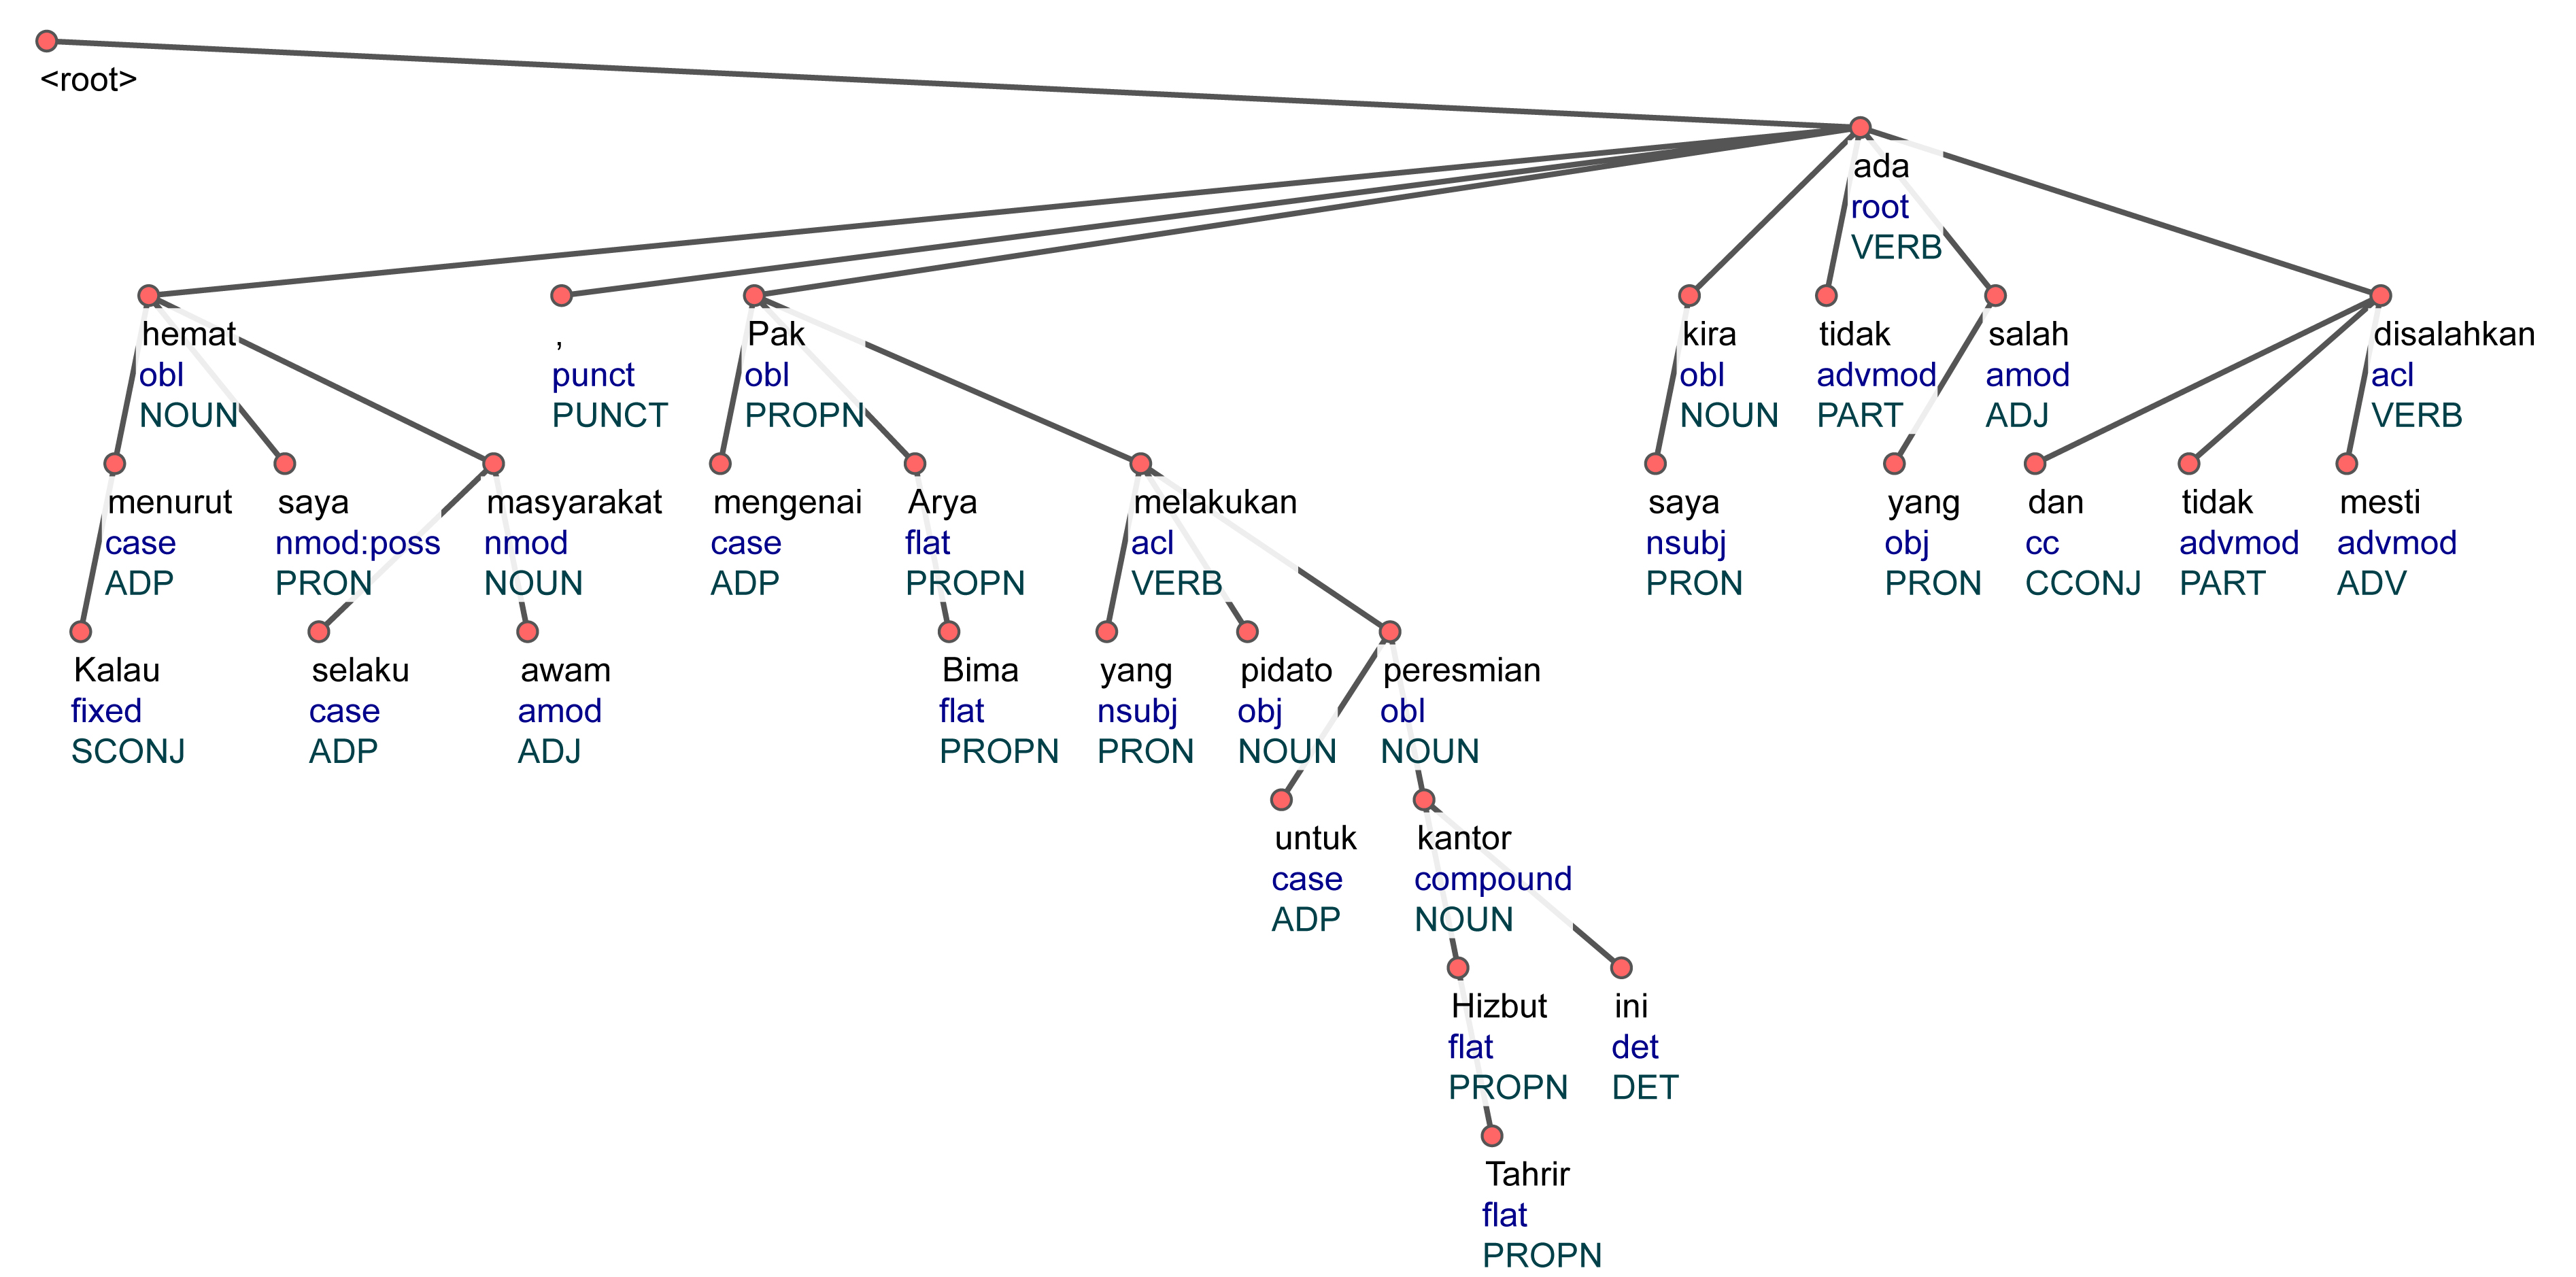
\includegraphics[width=1
	\textwidth] {pics/ls114.jpg} 
	\caption{Kalimat L31c pada data ragam lisan}
	\label{fig:ls114} 
\end{figure}

Posisi akar pada kalimat L31c (\pic~\ref{fig:ls114}) cenderung berada di akhir seperti pada kalimat L22. Hal ini berarti semua simpai-simpai cabang di bawah \textit{hemat} dan \textit{Pak} harus disimpan di dalam memori kerja sebelum akar verbal \textit{kira} direalisasikan. Di bawah simpai \textit{Pak}, terlihat adanya indikasi percabangan searah, yaitu relasi antara \textit{Pak} dengan \textit{melakukan} dan \textit{melakukan} dengan \textit{peresmian}, dan seterusnya. Namun seluruh relasi ini berada di bawah tautan utama antara \textit{ada} dengan \textit{Pak}, sehingga terjadi percabangan yang bersifat kombinasi antara searah dan beda arah. Kalimat L31c (\pic~\ref{fig:ls114}) memiliki DL sejauh 100 dan MDD sejauh 3,333 konstituen. Selisih nilai DL dari tautan-tautan dependensi positif dan negatif sangat besar yaitu -40. Nilai negatif ini menandakan jumlah bentuk relasi diakhiri induk yang jauh lebih besar dibandingkan sebaliknya. Tampak pada \pic~\ref{fig:ls114}, nilai negatif yang besar ini terutama disebabkan oleh tautan-tautan dependensi pada simpai pusat yang sangat jauh.

Kalimat L22 (\pic~\ref{fig:ls6521}), L31a (\pic~\ref{fig:ls1716}), L31b (\pic~\ref{fig:ls16}), dan L31c (\pic~\ref{fig:ls114}) sedikit berbeda satu sama lain, namun memiliki karakter utama yang serupa yang membedakannya dengan contoh-contoh kalimat pada data ragam tulis. Salah satunya adalah perbedaan posisi akar pada \pic~\ref{fig:ls6521}, \pic~\ref{fig:ls1716}, \pic~\ref{fig:ls16}, dan \pic~\ref{fig:ls114}. Berdasarkan beberapa visualisasi bank pohon struktur tersebut, perbedaan yang paling terlihat antara contoh-contoh pada ragam lisan dibandingkan dengan contoh-contoh pada ragam tulis adalah percabangannya yang terlihat lebih tidak konsisten. Meskipun tidak semua kalimat memiliki struktur seperti \pic~\ref{fig:ts2079} dan \pic~\ref{fig:ts2081}, mayoritas kalimat panjang pada data ragam tulis menunjukkan karakter yang lebih konsisten dalam hal pergerakan percabangannya. Pada data ragam lisan, terlihat banyak kombinasi antara percabangan searah dan beda arah serta letak posisi akar yang menyebar dari awal hingga akhir kalimat. Percabangan utama yang tersebar pada ketiga kalimat tersebut menunjukkan indikasi hubungan klausa yang tidak bersifat berlanjut, namun paralel. Kalimat L22 (\pic~\ref{fig:ls6521}), L31b (\pic~\ref{fig:ls16}) dan L31c (\pic~\ref{fig:ls114}) memiliki percabangan utama sebelum akar sehingga secara kolektif membentuk relasi dependensi utama yang negatif. Hal ini berarti seluruh informasi yang dibawa oleh klausa-klausa pada simpai dan percabangan sebelum akar harus disimpan dalam memori kerja dan menunggu realisasi akar yang mengandung informasi utama untuk dapat bermakna secara utuh \citep{hawkins2014cross}.

%%-----------------------------------------------------------------------------%
\subsection{Pengaruh panjang kalimat terhadap panjang dependensi kalimat dan rata-rata jarak dependensi antarkonstituen}
%%-----------------------------------------------------------------------------%
Berdasarkan percobaan acak yang dilakukan, langkah analisis pada bagian ini adalah melihat aspek-aspek yang mungkin mempengaruhi struktur kalimat sehingga memungkinkan terjadinya DLM dan DDM. Secara garis besar, analisis lanjutan untuk melihat aspek-aspek ini menghasilkan temuan strategi yang berkaitan dengan panjang kalimat, pengaturan urutan kata terkait pendekatan dan penempatan posisi, serta pengurangan valensi. Ketiga aspek besar ini menjawab pertanyaan-pertanyaan penelitian yang diajukan pada Bab 1. Langkah analisis pada bagian ini mencoba meninjau pengaruh panjang kalimat atau jumlah konstituen terhadap panjang dependensi kalimat dan jarak dependensi antarkonstituen serta struktur kalimat yang terbentuk dalam kedua korpus. Temuan utama yang muncul adalah dalam kondisi tertentu, perbandingan DL dan MDD antara kedua korpus data memiliki karakteristik yang berbeda. Rata-rata jumlah konstituen pada data ragam tulis berada antara 17 hingga 18 (\textit{mean} = 17,423) dan antara 10 hingga 11 konstituen (\textit{mean} = 10,859) pada ragam lisan dengan perbedaan yang signifikan (\textit{P} \textless 0,001). Perbedaan ini menunjukkan bahwa ada kecenderungan penutur memilih jumlah konstituen yang lebih sedikit saat merealisasikan kalimat secara lisan. Klasifikasi kalimat pendek, menengah, dan panjang dilakukan berdasarkan penelitian terdahulu dari \cite{gildea2015human}, \cite{futrell2015large}, \cite{wang2017effects}, serta \cite{liu2017dependency}. Berdasarkan data masing-masing penelitian tersebut, temuan-temuan yang didapat menyebutkan bahwa ada perbedaan perilaku dan karakteristik sintaksis yang dipengaruhi panjang kalimat. Berdasarkan klasifikasi panjang kalimat pada penelitian ini yang dilakukan bertitik tolak dari temuan-temuan tersebut, temuan analisis ini juga menemukan hasil yang serupa. 

Pada klasifikasi kalimat pendek (maksimal 10 konstituen dalam sebuah kalimat), perbedaan rata-rata panjang dan jarak dependensi antara ragam tulis dan lisan tampak dipengaruhi oleh pemusatan data ragam lisan. Kalimat-kalimat dalam kedua korpus sama-sama mengalami optimasi urutan kata yang menyebabkan terjadinya DLM dan DDM.  Namun, kecenderungan untuk menggunakan kalimat pendek menyebabkan data ragam lisan memiliki rata-rata DL dan MDD yang lebih pendek secara signifikan terutama hingga panjang kalimat sebanyak 5 konstituen. Pada pengamatan yang lebih dalam, ditemukan bahwa mulai jumlah konstituen sebanyak 6, data ragam tulis justru menunjukkan MDD yang lebih pendek secara signifikan. Tinjauan secara kualitatif mengindikasikan adanya perbedaan tingkat kedalaman dependensi antara kedua ragam pada contoh-contoh kalimat dengan jumlah konstituen sebanyak 4. Meskipun begitu, tidak ditemukan karakteristik struktur yang unik yang dapat membedakan keduanya secara signifikan tidak ditemukan. Struktur sintaksis dan pengaturan klausa bebas serta terikat pada kedua ragam juga tidak berbeda secara signifikan. Keserupaan ini mungkin disebabkan oleh keterbatasan jumlah konstituen dan bentuk-bentuk kalimat yang hanya mengandung satu klausa bebas sehingga kompleksitas kalimat-kalimat tersebut masih rendah. Meskipun begitu, terlihat indikasi adanya pengurangan atau reduksi konstituen pada data ragam lisan berupa subyek atau aktor pelaku. Tinjauan lebih dalam mengenai pengurangan valensi ini akan dibahas pada tahap analisis berikutnya.

Terdapat temuan yang menarik pada klasifikasi kalimat menengah, yaitu rata-rata DL dan MDD antara kedua korpus data yang berbanding terbalik. Rata-rata DL yang dihasilkan korpus data ragam lisan lebih pendek dibandingkan ragam tulis namun tidak berbeda secara signifikan. Sebaliknya, rata-rata MDD yang didapatkan korpus data ragam tulis lebih pendek dibandingkan ragam lisan dan berbeda secara signifikan. Asumsi perbedaan kedua nilai ini merupakan alasan mengapa kedua pendekatan digunakan pada penelitian ini. Berdasarkan temuan ini, perbedaan kedua pendekatan dapat memberikan temuan awal untuk melihat kesesuaiannya dalam mengukur efisiensi memori kerja yang tercermin pada struktur sintaksis sebuah kalimat. Rata-rata DL dan MDD yang berbanding terbalik ini mengindikasikan bahwa meskipun jumlah total panjang dependensi lebih jauh dalam satu klasifikasi karena jumlah konstituen yang lebih banyak, struktur kalimat yang lebih efisien dapat menghasilkan rata-rata jarak dependensi antarkonstituen yang lebih pendek. Dalam hal ini, data ragam tulis sudah mulai memperlihatkan struktur kalimat yang lebih efisien dibandingkan ragam lisan. Rata-rata jumlah konstituen antara kedua korpus data berbeda secara signifikan yang berarti pada klasifikasi ini, penutur masih memiliki kecenderungan atau preferensi untuk mengurangi panjang kalimat saat merealisasikan kalimat secara lisan. Berdasarkan temuan ini, muncul asumsi bahwa DL berguna untuk menggambarkan kompleksitas sebuah kalimat secara umum dan MDD berguna untuk mewakili bagaimana efisiensi struktur kalimat melalui tautan dependensi antarkonstituennya.

Pada klasifikasi kalimat panjang, kedua rata-rata DL dan MDD pada korpus data ragam tulis lebih pendek dibandingkan ragam lisan dan berbeda secara signfikan. Hal ini berarti ada indikasi bahwa struktur kalimat-kalimat ragam tulis lebih efisien dilihat baik dari segi kompleksitas kalimat maupun jarak antarkonstituen yang dapat mewakili bentuk strukturnya. Perbedaan rata-rata jumlah konstituen antara kedua korpus tidak signifikan yang berarti pada klasifikasi ini, tidak ada kecenderungan atau preferensi penutur terhadap panjang kalimat terkait ragam tertentu. Tinjauan lebih dalam dilakukan untuk mengamati struktur-struktur kalimat yang umum ditemukan pada kedua korpus data. Berdasarkan analisis yang bersifat kualitatif terhadap struktur kalimat-kalimat \pic~\ref{fig:ts3901}, \pic~\ref{fig:ts2079}, \pic~\ref{fig:ts2081}, \pic~\ref{fig:ls6521}, \pic~\ref{fig:ls1716}, \pic~\ref{fig:ls16}, dan \pic~\ref{fig:ls114}, terlihat ada perbedaan yang cukup mendasar antara kedua ragam. 

Pada struktur kalimat panjang ragam tulis, banyak ditemukan kalimat yang hanya memiliki satu simpai cabang terdekat meskipun mengandung banyak klausa terikat sehingga kompleksitas kalimat tergolong tinggi. Hal ini juga terlihat pada berbedaan tingkat kedalaman dependensi antara kedua ragam. Pengaturan urutan kata pada bentuk struktur sintaksis seperti pada ragam tulis mencerminkan percabangan searah dan mengakibatkan hubungan-hubungan antarklausanya bersifat berlanjut. Contoh-contoh pada ragam tulis juga menunjukkan jumlah tautan dependensi antara dua konstituen yang berdampingan yang lebih banyak dibandingkan pada ragam lisan. Berkaitan dengan teori dependensi \citep{tesniere1959elements, hawkins2014cross, gildea2010grammars}, hubungan seri ini dilakukan untuk menambahkan informasi secara bertahap sehingga tautan dependensinya lebih pendek. 

Struktur sintaksis yang ditemukan pada kalimat-kalimat ragam tulis ini juga memilki posisi akar relatif paling awal. Oleh karena itu, seiring jalannya kalimat direalisasikan, informasi yang diproduksi setelahnya bersifat tambahan karena akar (konstituen yang mengandung informasi utama) sudah direalisasikan sejak awal. Berbeda dengan ragam tulis, struktur-struktur kalimat dalam data ragam lisan ditemukan tidak konsisten dan berbeda satu sama lain. Posisi akar dapat berada di depan, tengah, maupun akhir dan banyak ditemukan kalimat dengan banyak simpai cabang pada tingkat tautan dependensi utama. Relasi $parataxis$ dengan akar juga ditemukan yang berarti simpai cabang memiliki kualitas diskursus dan dapat menjadi kalimat lepas namun bergabung menjadi satu kalimat. Simpai-simpai cabang ini juga mengakibatkan klausa-klausa terikat tersebar secara paralel yang mungkin juga menyebabkan tingkat kedalaman dependensi pada ragam lisan ini lebih dangkal dibandingkan ragam tulis. Pada beberapa kalimat, ditemukan kombinasi percabangan yang bersifat searah maupun beda arah, tetapi kemunculannya juga tidak konsisten. Terutama pada akar yang berada di akhir kalimat, klausa-klausa yang terikat pada simpai-simpai cabang sebelumnya harus disimpan dulu di memori kerja hingga akar yang mengandung informasi utama direalisasikan dalam kalimat. 

Terdapat satu kalimat contoh dari korpus ragam tulis yang panjang dan jarak dependensinya sama dengan salah satu kalimat dari korpus ragam lisan. Namun, kedua kalimat ini memiliki struktur sintaktis yang jauh berbeda. Perbedaan utama kedua kalimat tersebut terletak pada tingkat kedalaman dependensi yang diakibatkan oleh perbedaan konstruksi kalimat. Perbedaan ini juga dapat terlihat pada visualisasi bank pohon struktur dependensi kedua kalimat. Kalimat ragam tulis menunjukkan percabangan yang bergerak searah semakin ke bawah sehingga menghasilkan tingkat kedalaman dependensi yang berlapis-lapis. Sementara itu, kalimat ragam lisan menunjukkan percabangan yang menyebar dengan pembagian cabang yang cukup merata sehingga menghasilkan tingkat kedalaman dependensi yang lebih dangkal. Temuan ini sangat menarik karena menimbulkan pertanyaan bahwa meskipun panjang dan jarak dependensi dua kalimat sama, apakah penutur tetap akan cenderung memilih satu bentuk konstruksi dibandingkan yang lain. Pertanyaan ini membutuhkan penelitian lanjutan yang melibatkan uji persepsi.

Secara umum, perbandingan analisis pada ketiga klasifikasi memberikan informasi yang berarti. Perbedaan yang ditemukan pada ketiganya menandakan bahwa panjang kalimat berpengaruh terhadap panjang dependensi kalimat dan rata-rata jarak dependensi antarkonstituen. Namun, perbedaan karakter struktur sintaksis pada korpus data ragam tulis dan lisan baru terlihat jelas pada kalimat dengan kompleksitas lebih tinggi jumlah konstituen yang lebih banyak. \cite{wang2017effects} menemukan dalam penelitiannya bahwa data ragam tulis yang ditujukan untuk percakapan lisan (sebagai contoh dialog film) memiliki MDD yang lebih pendek dibandingkan teks yang lebih formal. \cite{wang2017effects} menindaklanjuti kajian yang dilakukan \cite{hiranuma1999syntactic} dan \cite{liu2009chinese} mengajukan asumsi bahwa pada teks yang semakin formal (berdasarkan data yang digunakan) lebih sulit secara sintaktis. Dalam penelitian ini, temuan serupa terjadi pada klasifikasi kalimat pendek (\textless= 5 konstituen) di mana ragam lisan memiliki DL dan MDD yang lebih pendek. Temuan serupa didapatkan oleh \cite{wang2017effects}, yang mengindikasikan bahwa kalimat-kalimat ragam lisan pada klasifikasi ini lebih mudah dimengerti secara sintaktis. Namun, asumsi ini tidak berlaku pada kalimat yang lebih panjang. 

Berdasarkan data yang dikumpulkan pada penelitian ini, pada klasifikasi menengah dan panjang, teks yang lebih formal (ragam tulis) justru menunjukkan efisiensi kalimat yang lebih tinggi mulai dari jumlah konstituen sebanyak 6 hingga 40. Merujuk pada \pic~\ref{fig:lisantulis_DL} dan \pic~\ref{fig:lisantulis_MDD}, kedua grafik menunjukkan gerak garis regresi yang berkebalikan antara ragam lisan dan tulis pada titik sekitar panjang kalimat sebanyak 40 konstituen. Namun, signifikansi yang melemah dan cenderung berbalik pada panjang kalimat di atas 40 konstituen mungkin disebabkan oleh persebaran data kedua korpus yang sangat sedikit pada rentang tersebut, terutama pada data ragam lisan. Penelitian lanjutan untuk rentang panjang kalimat tersebut membutuhkan data dengan jumlah yang cukup besar dan seimbang pada kedua korpus, namun kalimat yang sangat panjang cukup jarang ditemukan dalam ragam lisan. Hal ini dapat dikaitkan dengan kecenderungan pada ragam lisan untuk menggunakan kalimat-kalimat yang pendek. Analisis kualitatif terhadap perbedaan karakteristik sintaksis pada klasifikasi kalimat panjang memperlihatkan secara jelas bagaimana perbedaan struktur kalimat pada kedua ragam, terutama terkait tingkat kedalaman dependensi, tautan dependensi dari dua konstituen yang berdampingan, dan reduksi sintaktik atau reduksi konstituen pada ragam lisan yang menyebabkan panjang kalimat menjadi lebih pendek.

%%-----------------------------------------------------------------------------%
\section{Direksionalitas induk dan valensi akar verbal}
%%-----------------------------------------------------------------------------%
Pada pembahasan temuan-temuan di atas, sudah dibahas sedikit mengenai struktur kalimat terkait posisi akar dan pola percabangannya. Seperti yang dijelaskan sebelumnya, belum ada konvensi mengenai direksionalitas induk terkait hierarki dan pengolahan dalam memori kerja. Jarak dependensi positif dihasilkan dari bentuk relasi induk sebelum konstituen terikat, dan sebaliknya, nilai dependensi negatif dihasilkan dari bentuk relasi induk setelah konstituen terikat. Bahasa Indonesia memiliki urutan kata yang cenderung bebas \citep{sneddon2010indonesian} dan dalam aturan tata bahasa yang mengadopsi prinsip struktur frasa, banyak urutan kata dalam aturan frasa yang memiliki kepala (\textit{head}) mendahului pewatas (\textit{modifier}) \citep{sneddon2010indonesian}. Akan tetapi, teori struktur frasa berbeda dengan dependensi dan belum ada penelitian yang melihat relasi induk dan konstituen terikat terkait arah dan posisi induknya (direksionalitas induk). 

Hipotesis yang digunakan pada beberapa penelitian yang melihat Pengurangan Panjang Dependensi (DLM) \citep{futrell2015large} serta Pengurangan Jarak Dependensi (DDM) \citep{liu2017dependency} menyebutkan bahwa kebebasan urutan kata ini mungkin dimanfaatkan oleh penutur menjadi strategi utama dalam menghasilkan kalimat yang efisien terutama mengenai penempatan konstituen pada posisi tertentu dalam urutan konstituen sebuah kalimat. Pada pembahasan ini, penghitungan DL tautan dependensi positif dipisahkan dengan tautan dependensi negatif. Bagian pertama analisis DL positif dan negatif melibatkan relasi dari semua konstituen dalam kalimat. DL positif dan negatif ini memberikan gambaran kasus tautan akar atau induk dengan konstituen terikat secara umum dan berkontribusi untuk membentuk asumsi kecenderungan karakteristik bahasa dilihat dari direksionalitas induknya \citep{wang2017effects}. 

\begin{figure}
\centering

\begin{subfigure}{.8\linewidth}
  \centering
  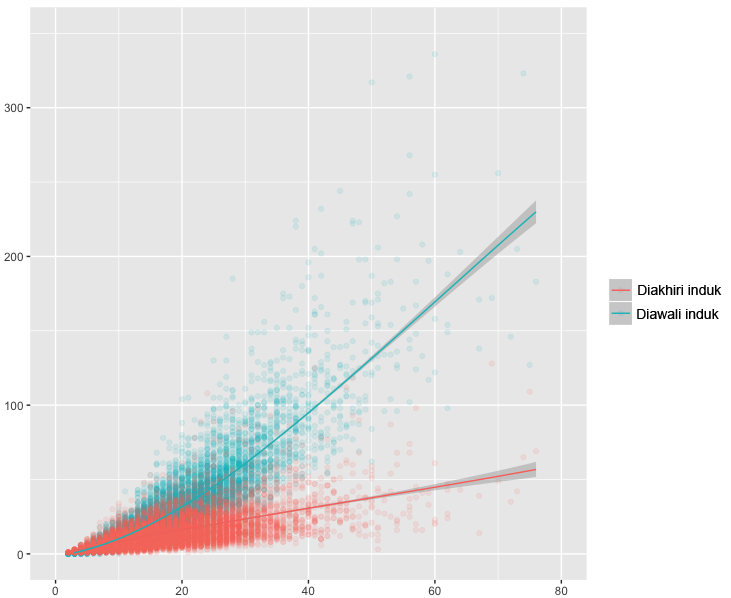
\includegraphics[width=1\linewidth] {pics/tulis_DLposneg.png} 
	\caption{Data ragam tulis}
	\label{fig:tulis_DLposneg} 
\end{subfigure}
%
\begin{subfigure}{.8\linewidth}
  \centering
  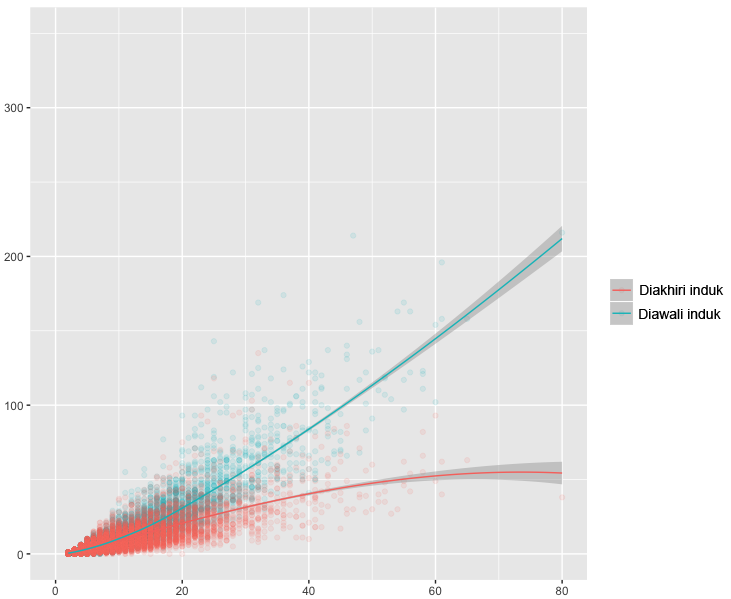
\includegraphics[width=1\linewidth]{pics/lisan_DLposneg.png} 
	\caption{Data ragam lisan}
	\label{fig:lisan_DLposneg} 
\end{subfigure}

\caption{Grafik panjang dependensi positif dan negatif data ragam tulis dan lisan}
\label{fig:DL_posneg}
\end{figure}

Berdasarkan \pic~\ref{fig:tulis_DLposneg} dan \pic~\ref{fig:lisan_DLposneg}, kedua korpus data menunjukkan garis regresi tautan dependensi positif yang berada jauh di atas garis regresi tautan dependensi negatif dan pada kalimat dengan jumlah konstituen yang semakin banyak, jarak antara keduanya semakin besar. Seperti yang dijelaskan sebelumnya, DL cukup sensitif terhadap panjang kalimat dan keduanya memiliki hubungan linear. Dalam sebuah kalimat, perbandingan jumlah bentuk relasi diawali dan diakhiri induk saling berkaitan. Hal ini berarti ada kecenderungan preferensi terhadap bentuk relasi diawali induk dan menandakan kesesuaian data observasi dengan tata bahasa yang berlaku. Namun, pada grafik DL ragam lisan (\pic~\ref{fig:lisan_DLposneg}), jarak garis regresi tautan dependensi positif dan negatif terlihat lebih dekat dibandingkan ragam tulis. Grafik ini juga memperlihatkan adanya kurva parabola terbuka ke bawah sehingga muncul asumsi adanya nilai tertinggi atau ambang batas (\textit{threshold}) terhadap panjang tautan dependensi negatif pada korpus data ragam lisan. Berdasarkan korpus data yang terkumpul, dugaan ambang batas tautan dependensi negatif ini menimbulkan asumsi bahwa mulai panjang kalimat tertentu, total tautan dependensi negatif dalam sebuah kalimat mungkin tidak akan melebihi nilai tertentu juga. 

\begin{table}
\begin{center}
\begin{small}
\caption{Frekuensi panjang dependensi positif dan negatif}  \label{tab:DLposneg}
\begin{tabular}{ | p{2cm} | p{2cm} | p{2cm} | p{2cm} | p{2cm} |}
\hline
Jumlah konstituen & Ragam tulis (+ \textgreater -) & Ragam tulis (+ \textless -) & Ragam lisan (+ \textgreater -) & Ragam lisan (+ \textless -) \\ \hline
\textless= 5 & 164 & 221 & 1188 & 1354 \\ \hline
6 - 10 & 992 & 646 &1469 & 1349 \\ \hline
11 - 20 & 3145 & 952 & 1858 & 1014 \\ \hline
21 - 30 & 1854 & 200 & 644 & 166 \\ \hline
31 - 40 & 558 & 36 & 204 & 37 \\ \hline
\textgreater 40 & 201 & 5 & 89 & 7 \\ \hline
 \end{tabular}
 \end{small}
 \end{center}
 \end{table}
 
\tab~\ref{tab:DLposneg} berisi frekuensi kalimat dengan melihat apakah kalimat tersebut memiliki DL positif yang lebih jauh atau sebaliknya. Hal ini berarti kalimat yang memiliki DL positif dan negatif sama jauh tidak diikutsertakan dalam analisis. Jumlah kalimat dalam \tab~\ref{tab:DLposneg} dihitung berdasarkan selisih panjang dependensinya. Berdasarkan tabel ini, kalimat yang DL positifnya lebih besar dari negatif ditemukan lebih banyak mulai dari panjang kalimat 6 konstituen. Hal ini memperlihatkan adanya kecenderungan terhadap bentuk relasi diawali induk. Selain itu, rasio perbandingan pada ragam tulis jauh lebih besar dibandingkan ragam lisan. Pada kategori kalimat terpanjang, jumlah kalimat yang DL positifnya lebih besar dapat mencapai 40 kali lebih banyak.  Temuan ini menunjukkan bahwa bentuk relasi diawali induk memiliki total jarak-jarak dependensi yang lebih besar dibandingkan bentuk relasi sebaliknya. Seiring bertambahnya jumlah konstituen, rasio frekuensi tautan dependensi positif dan negatif semakin besar pada kedua ragam. Namun, perbedaan rasio dari setiap kategori jumlah konstituen pada ragam lisan tidak sejauh ragam tulis. 

\begin{table}
\begin{center}
\begin{small}
\caption{Frekuensi tautan dependensi positif dan negatif}  \label{tab:tautanposneg}
\begin{tabular}{ | p{2cm} | p{2cm} | p{2cm} | p{2cm} | p{2cm} |}
    \hline
Jumlah konstituen & Ragam tulis (+) & Ragam tulis (-) & Ragam lisan (+) & Ragam lisan (-) \\ \hline
\textless= 5 & 677 & 700 & 2841 & 2764 \\ \hline
6 - 10 & 7023 & 5715 & 7649 & 6918 \\ \hline
11 - 20 & 35597 & 24426 & 15554 & 12898 \\ \hline
21 - 30 & 31036 & 18163 & 7564 & 5939 \\ \hline
31 - 40 & 12904 & 6968 & 3232 & 2414 \\ \hline
\textgreater 40 & 6583 & 3240 & 1928 & 1426 \\ \hline
   \end{tabular}
   \end{small}
\end{center}
\end{table}

\tab~\ref{tab:tautanposneg} merupakan tabel yang berisi frekuensi tautan dependensi positif dan negatif dalam kedua korpus data. Frekuensi ini hanya menggambarkan jumlah kemunculan tautan dan tidak memiliki jarak dependensi. Pada tabel ini, tautan-tautan dependensi tidak dikelompokkan per kalimat sehingga dapat memberikan gambaran jumlah tautan yang ada dalam keseluruhan korpus. Data ragam tulis menunjukkan bahwa mulai dari panjang kalimat 6 konstituen, frekuensi tautan dependensi negatif lebih sedikit dibandingkan tautan dependensi positif. Meskipun begitu, tautan dependensi positif lebih banyak pada semua klasifikasi dalam ragam lisan. Pada kategori kalimat terpanjang dalam ragam tulis, frekuensi tautan dependensi positif dapat mencapai dua kali tautan dependensi negatif. Sementara pada ragam lisan, perbandingan terbesar hanya mencapai 1,35 banding 1 sehingga juga menunjukkan indikasi bahwa kecenderungan bentuk relasi diawali induk lebih terlihat pada data ragam tulis. Rasio dengan jumlah tautan dependensi pada tabel ini memperlihatkan perbandingan yang tidak seekstrim rasio dengan jumlah kalimat pada tabel sebelumnya. Hal ini menandakan bahwa pada kalimat yang semakin panjang, bentuk relasi diawali induk lebih banyak digunakan oleh penutur bahasa Indonesia dan dalam satu kalimat, panjang dependensi dari tautan dependensi positif dapat memiliki nilai yang jauh lebih besar.

\begin{table}
\begin{center}
\begin{footnotesize}
\caption{Jarak dependensi seluruh tautan antarkonstituen}  \label{tab:deskriptif-konstituen}
\begin{tabular}{| c | llll | llll | l |}
\hline
 & \multicolumn{4}{c |}{+} & \multicolumn{4}{c |}{-} & \\  \cline{2-9}  
Panjang kalimat & min & med	& max & mean & min & med & max & mean & \\ \cline{1-10}  
\textless= 5 	& 1 & 1 & 4 & 1,409 	& 1 & 1 & 4 & 1,606 & \multirow{6}{*}{Tulis}\\
6 - 10 		& 1 & 1 & 9 & 1,866 	& 1 & 1 & 9 & 1,948 & \\
11 - 20 		& 1 & 1 & 19 & 2,468 & 1 & 1 & 19 & 2,147 & \\
21 - 30 		& 1 & 1 & 29 & 2,971 & 1 & 1 & 29 & 2,241 & \\ 
31 - 40 		& 1 & 1 & 39 & 3,597 & 1 & 1 & 37 & 2,299 & \\
\textgreater 40 & 1 & 1 & 68 & 4,22 	& 1 & 1 & 55 & 2,282 & \\ 
\hline
\textless= 5 	& 1 & 1 & 4 & 1,466 	& 1 & 1 & 4 & 1,534 & \multirow{6}{*}{Lisan}\\
6 - 10 		& 1 & 1 & 9 & 1,933 	& 1 & 1 & 9 & 2,071 & \\
11 - 20 		& 1 & 2 & 19 & 2,535 & 1 & 1 & 19 & 2,321 & \\
21 - 30 		& 1 & 2 & 28 & 3,263 & 1 & 1 & 27 & 2,5 & \\ 
31 - 40 		& 1 & 2 & 37 & 3,718 & 1 & 1 & 32 & 2,657 & \\
\textgreater 40 & 1 & 2 & 66 & 4,067 	& 1 & 1 & 46 & 2,438 & \\ 
\hline
   \end{tabular}
   \end{footnotesize}
\end{center}
\end{table}

 \tab~\ref{tab:deskriptif-konstituen} mencakup jarak dependensi dari seluruh tautan yang ada dalam kedua korpus data dan tidak dikelompokkan berdasarkan kalimatnya. Tabel ini mendukung temuan sebelumnya dan memperlihatkan bahwa rata-rata jarak dependensi positif lebih jauh dibandingkan dependensi negatif, terutama pada kalimat yang semakin panjang. Perbandingan ini mulai terlihat pada kategori panjang kalimat 11 konstituen dan meningkat seiring bertambahnya jumlah konstituen. Pada kategori kalimat terpanjang, perbandingan jarak antara dependensi positif dan negatif juga semakin jauh. Pada \tab~\ref{tab:deskriptif-konstituen}, terlihat bahwa hampir semua nilai tengah jarak dependensi sama atau sangat mendekati nilai minimum terutama pada ragam tulis. Hal ini menunjukkan bahwa ada kecenderungan banyaknya dua konstituen yang saling berdampingan sehingga menghasilkan nilai minimum atau 1. Pada kategori kalimat terpanjang dalam kedua ragam (\textgreater 40 konstituen), rata-rata jarak dependensi negatif lebih pendek dibandingkan kategori sebelumnya (31-40 konstituen). Meskipun demikian, perbedaan yang signifikan (\textit{P} \textless 0.05) hanya ditemukan pada ragam lisan. Hal ini berarti pada ragam lisan, mulai panjang kalimat tertentu (yang berdasarkan data ini adalah sekitar 40 konstituen) jarak dependensi negatif tidak akan melebihi nilai tertentu. 

\begin{table}
\begin{center}
\begin{footnotesize}
\caption{Rata-rata jarak dependensi positif dan negatif}  \label{tab:deskriptif-mdd}
\begin{tabular}{| c | llll | llll | l |}
\hline
 & \multicolumn{4}{c |}{+} & \multicolumn{4}{c |}{-} & \\  \cline{2-9}  
Panjang kalimat & min 	& med	& max 	& mean 	& min 	& med 	& max 	& mean 	& \\ \cline{1-10}  
\textless= 5 	& 1 		& 1 		& 3,5	 	& 1,372 	& 1 		& 1,5 	& 4	 	& 1,545 	&\multirow{6}{*}{Tulis}\\
6 - 10 		& 1 		& 1,667	& 5,2 	& 1,839 	& 1 		& 1,667 	& 9	 	& 1,895 	& 	\\
11 - 20 		& 1 		& 2,25 	& 7,25 	& 2,432 	& 1 		& 1,875 	& 10	 	& 2,117 	& 	\\
21 - 30 		& 1 		& 3,765 	& 10,278 	& 2,97 	& 1 		& 2 		& 12,75	& 2,212 	& 	\\ 
31 - 40 		& 1,458 	& 3,368 	& 9,933	& 3,595 	& 1 		& 2 		& 8		& 2,272 	& 	\\
\textgreater 40 	& 1,929 	& 3,756	& 10,567 	& 4,154 	& 1 		& 2 		& 7,111	& 2,258 	& 	\\ 
\hline
\textless= 5 	& 1 		& 1 		& 4	 	& 1,378 	& 1 		& 1,33 	& 4		& 1,456 	& \multirow{6}{*}{Lisan}\\
6 - 10 		& 1 		& 1,714	& 5,6 	& 1,867 	& 1 		& 1,8		& 9		& 2,003 	& \\
11 - 20 		& 1 		& 2,286 	& 9,625 	& 2,479 	& 1 		& 2 		& 6,818	& 2,255 	& \\
21 - 30 		& 1,4 	& 3	 	& 8,412 	& 3,252	& 1 		& 2,188	& 8,636	& 2,447 	& \\ 
31 - 40 		& 1,556 	& 3,512 	& 7,25	& 3,719 	& 1 		& 2,27	& 8,803	& 2,612 	& \\
\textgreater 40 	& 2,174 	& 3,865	& 6,895 	& 3,957 	& 1,059 	& 2,294	& 4,2		& 2,363 	& \\ 
\hline
   \end{tabular}
   \end{footnotesize}
\end{center}
\end{table}

Nilai-nilai pada \tab~\ref{tab:deskriptif-mdd} didapatkan dengan menghitung MDD positif dan negatif pada setiap kalimat. Distribusi nilai minimum, tengah dan maksimum pada ragam lisan lebih merata dibandingkan ragam tulis yang nilai tengahnya terlihat lebih mendekati nilai minimum terutama pada kalimat yang semakin panjang (mulai terlihat pada panjang kalimat 11 konstituen). Mulai panjang kalimat tersebut, rata-rata MDD pada ragam tulis juga terlihat lebih pendek. Hal ini mendukung temuan sebelumnya bahwa dibandingkan ragam lisan, pada kalimat yang lebih panjang, bahasa Indonesia ragam tulis lebih memperlihatkan upaya untuk meningkatkan efisiensi kalimat dengan mendekatkan konstituen-konstituen yang memiliki tautan dependensi sehingga menghasilkan panjang dan jarak dependensi yang lebih pendek. Seperti \tab~\ref{tab:deskriptif-konstituen}, tabel ini juga memperlihatkan indikasi bahwa tautan dependensi negatif memiliki rata-rata jarak yang lebih pendek. Rasio perbandingan dependensi positif dan negatif pada ragam lisan juga tidak seekstrim data ragam tulis. 

\begin{figure}
\centering

\begin{subfigure}{.4\linewidth}
  \centering
  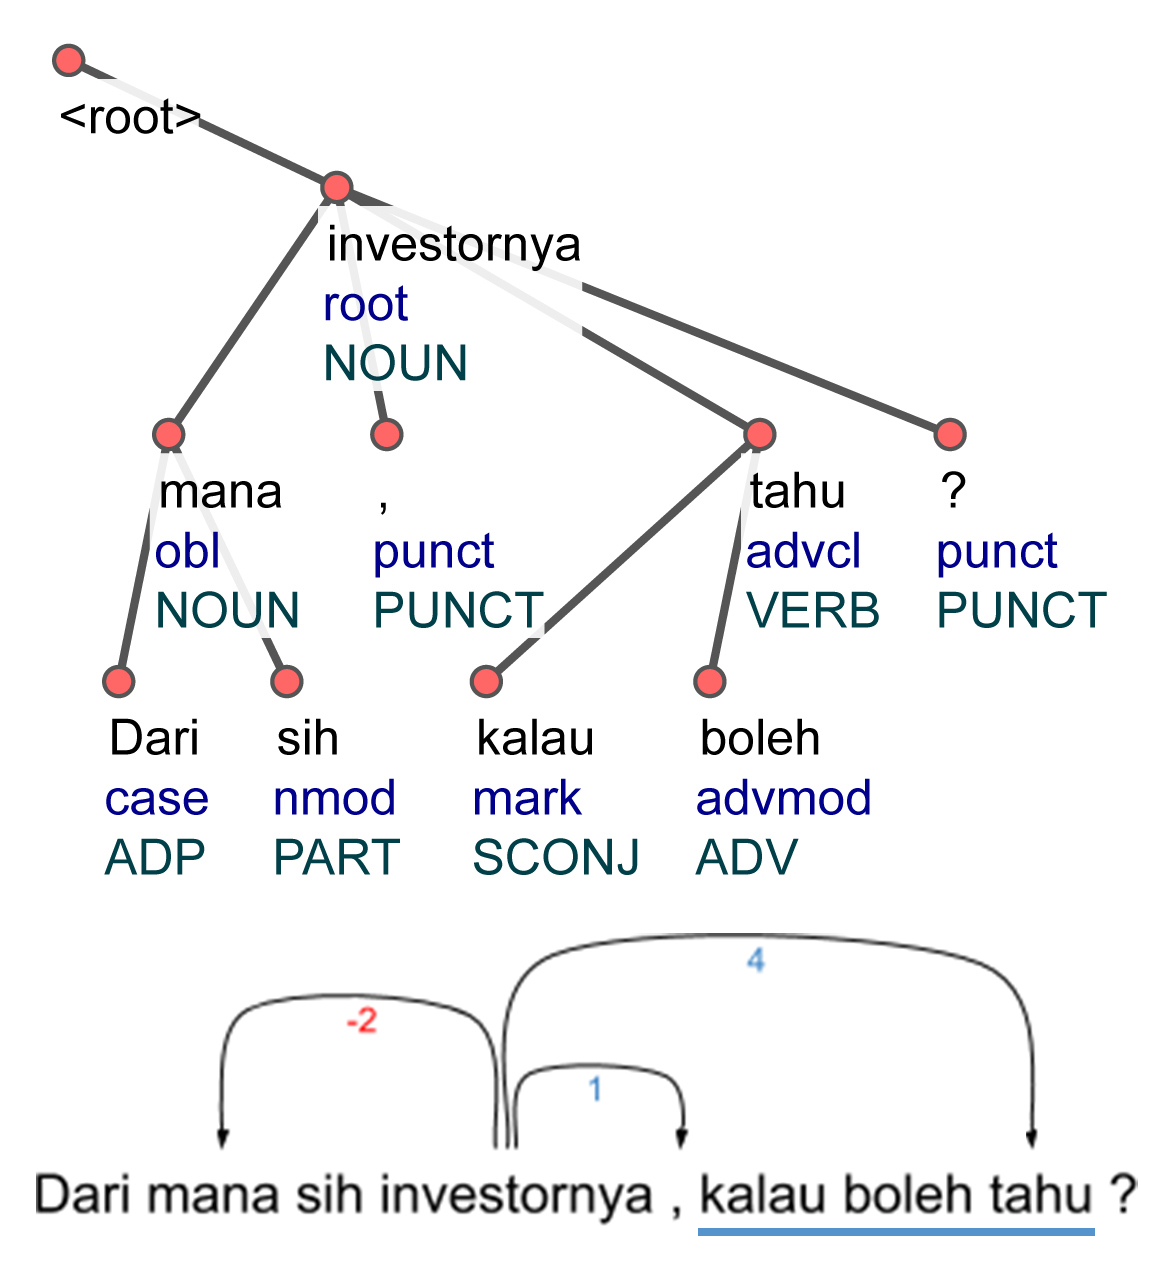
\includegraphics[width=1\linewidth] {pics/ls1436.jpg} 
	\caption{L\textit{akar}a}
	\label{fig:ls1436} 
\end{subfigure}
%
\begin{subfigure}{.58\linewidth}
  \centering
  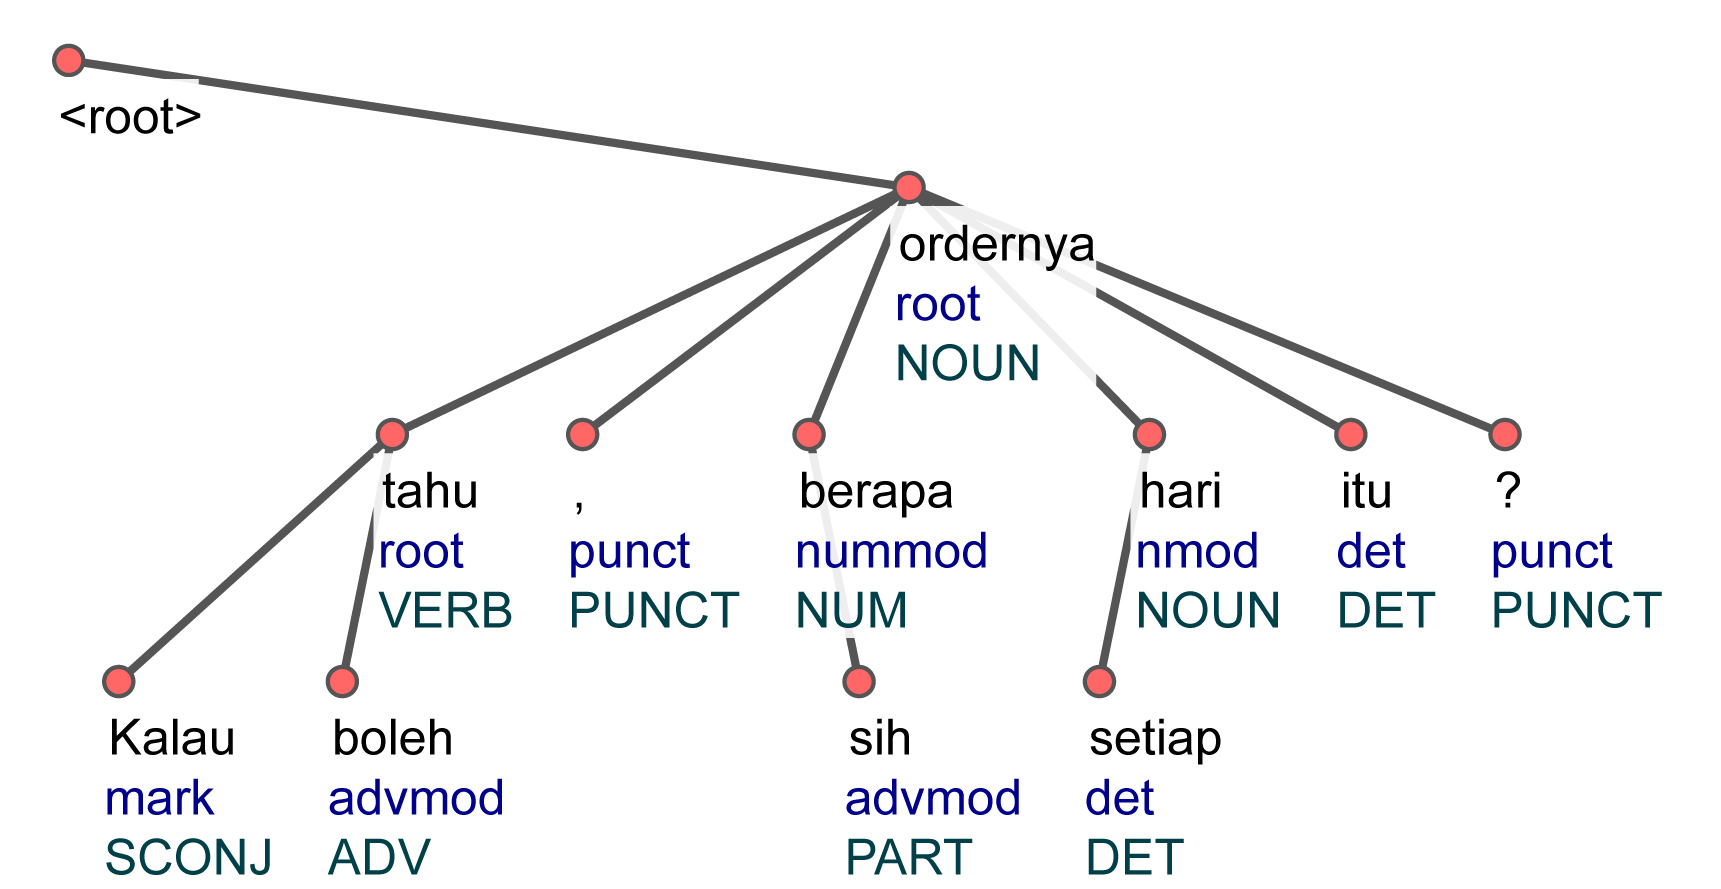
\includegraphics[width=1\linewidth]{pics/ls1460.jpg} 
	\caption{L\textit{akar}b}
	\label{fig:ls1460} 
\end{subfigure}

\caption{Contoh perbedaan penempatan klausa pada data ragam lisan}
\label{fig:akarcontoh}
\end{figure}


Salah satu bagian analisis penelitian ini berkaitan dengan valensi sebuah konstituen dalam kalimat. \pic~\ref{fig:akarcontoh} menampilkan contoh perbedaan penempatan klausa terikat \textit{kalau boleh tahu}. Sesuai dengan batasan penelitian ini, bagian analisis ini difokuskan hanya pada simpai pusat dengan kelas kata akar berupa kata kerja atau verba. \pic~\ref{fig:ls1436} dan \pic~\ref{fig:ls1460} merupakan dua kalimat yang ditemukan pada korpus data ragam lisan. Klausa terikat \textit{kalau boleh tahu} pada kalimat L\textit{akar}a (\pic~\ref{fig:ls1436}) dan L\textit{akar}b (\pic~\ref{fig:ls1460}) berada pada posisi yang berbeda namun tidak mengubah makna kalimat. Contoh serupa juga sempat dijabarkan oleh \cite{sneddon2010indonesian} dalam buku \textit{Indonesian Reference Grammar} Pada kalimat L\textit{akar}b, konstituen-konstiuen yang membentuk klausa \textit{kalau boleh tahu} secara kolektif memiliki relasi dependensi utama negatif terhadap akar \textit{ordernya}. Sesuai dengan bentuk relasi induk dan konstituen terikat berdasarkan teori dependensi yang dijabarkan oleh \cite{tesniere1959elements}, klausa terikat pada posisi awal kalimat ini harus disimpan dalam memori kerja terlebih dahulu hingga akar direalisasikan. Karena akar mengandung informasi utama, perbedaan kedua kalimat ini juga dapat memberikan sedikit gambaran bagaimana perbedaan proses memori kerja terkait penyimpanan informasi yang merupakan argumen inti kalimat.

\begin{figure}
\centering

\begin{subfigure}{.8\linewidth}
  \centering
  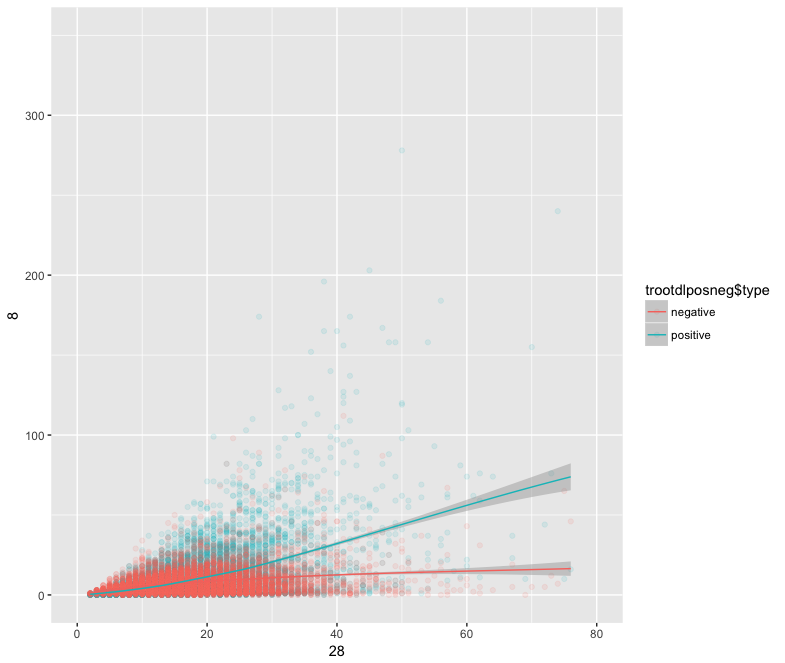
\includegraphics[width=1\linewidth] {pics/tulisroot_DLposneg.png} 
	\caption{Data ragam tulis}
	\label{fig:tulisroot_DLposneg} 
\end{subfigure}
%
\begin{subfigure}{.8\linewidth}
  \centering
  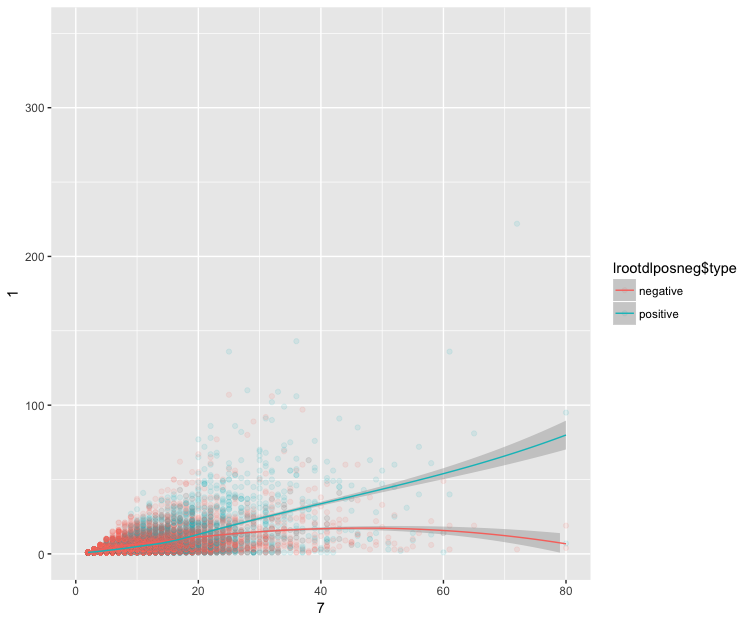
\includegraphics[width=1\linewidth]{pics/lisanroot_DLposneg.png} 
	\caption{Data ragam lisan}
	\label{fig:lisanroot_DLposneg} 
\end{subfigure}

\caption{Grafik panjang dependensi positif dan negatif pada simpai pusat data ragam tulis dan lisan}
\label{fig:rootDL_posneg}
\end{figure}

\pic~\ref{fig:tulisroot_DLposneg} dan \pic~\ref{fig:lisanroot_DLposneg} merupakan grafik DL positif dan negatif yang didapat pada simpai pusat kalimat dengan akar berupa verba. Kalimat dengan akar verbal ditemukan sebanyak 84,61\% atau sebanyak 7874 kalimat pada data ragam tulis dan 70,91\% atau sebanyak 7239 kalimat pada data ragam lisan. Mayoritas frekuensi kemunculan akar verbal ini dianalisis untuk melihat bagaimana penutur menyusun informasi utama dengan meninjau tautan-tautan dependensi utama (simpai pusat). Oleh sebab itu, semua klausa yang mungkin terikat pada simpai cabang dianggap mengikuti induknya seperti pada contoh uraian relasi klausa \textit{kalau boleh tahu} dan akarnya di atas (\pic~\ref{fig:akarcontoh}). \pic~\ref{fig:rootDL_posneg} menunjukkan adanya konsistensi pada tingkat tautan dependensi utama dan keseluruhan kalimat. Grafik ini memperlihatkan bahwa penutur juga cenderung memilih untuk menekan penggunaan bentuk relasi diakhiri induk terutama pada kalimat panjang. Berbeda dengan \pic~\ref{fig:DL_posneg} yang pada klasifikasi kalimat menengah sudah cukup terlihat perbedaan antara DL positif dan negatif, grafik ini menunjukkan DL positif dan negatif saling tumpang tindih sehingga perlu ditinjau lebih dalam. Meskipun begitu, serupa dengan \pic~\ref{fig:DL_posneg}, garis regresi nilai DL negatif mengindikasikan adanya ambang batas pada nilai tertentu terutama pada data ragam lisan.

\begin{table}
\begin{center}
\begin{small}
\caption{Frekuensi selisih panjang dependensi positif dan negatif pada simpai pusat akar verbal}  \label{tab:DLpusatposneg}
\begin{tabular}{ | p{2cm} | p{2cm} | p{2cm} | p{2cm} | p{2cm} |}
    \hline
Jumlah konstituen & Ragam tulis (+ \textgreater -) & Ragam tulis (+ \textless -) & Ragam lisan (+ \textgreater -) & Ragam lisan (+ \textless -) \\ \hline
\textless= 5 	& 57	 	& 180 	& 393 & 1008 \\ \hline
6 - 10 		& 475 	& 796	& 655 & 1356 \\ \hline
11 - 20 		& 1638	& 1804	& 964 & 1336 \\ \hline
21 - 30 		& 1028	& 778	& 384 & 291 \\ \hline
31 - 40 		& 325	& 177	& 121 & 85 \\ \hline
\textgreater 40 	& 137	& 37	 	& 61 & 30 \\ \hline
   \end{tabular}
   \end{small}
\end{center}
\end{table}

\tab~\ref{tab:DLpusatposneg} berisi jumlah-jumlah kalimat dengan melihat apakah kalimat tersebut memiliki DL postif yang lebih jauh atau sebaliknya pada simpai pusat yang memiliki akar verbal. Sebagai contoh, simpai pusat kalimat L4 \textit{Hasil surveynya cukup mengejutkan} pada \pic~\ref{fig:ls1102} memiliki 3 konstituen yang saling bertautan, yaitu \textit{mengejutkan} dengan \textit{hasil} dan \textit{mengejutkan} dengan \textit{cukup}. Kedua tautan memiliki bentuk relasi diakhiri induk dan memiliki DL negatif lebih jauh dibandingkan DL positif. Berbeda dengan \tab~\ref{tab:DLposneg}, kalimat yang DL positifnya lebih jauh ditemukan lebih banyak pada kalimat-kalimat panjang (mulai 21 konstituen). Pada ragam tulis, frekuensi keseluruhan hampir seimbang sedangkan pada ragam lisan cukup berbeda jauh (total frekuensi di mana DL negatif lebih jauh dari DL positif sebanyak dua kali lipat dibandingkan sebaliknya). 

\begin{table}
\begin{center}
\begin{small}
\caption{Frekuensi tautan dependensi positif dan negatif pada simpai pusat akar verbal}  \label{tab:tautanpusatposneg}
\begin{tabular}{ | p{2cm} | p{2cm} | p{2cm} | p{2cm} | p{2cm} |}
    \hline
Jumlah konstituen & Ragam tulis (+) & Ragam tulis (-) & Ragam lisan (+) & Ragam lisan (-) \\ \hline
\textless= 5 	& 201	& 412 & 1204 & 2151 \\ \hline
6 - 10 		& 1917	& 2532 & 2998 & 4433 \\ \hline
11 - 20 		& 6914 	& 7144 & 4753 & 5570 \\ \hline
21 - 30 		& 4455	& 3691 & 1869 & 1754 \\ \hline
31 - 40 		& 1528	& 1031 & 540 & 461 \\ \hline
\textgreater 40 	& 625	& 321 & 315 & 258 \\ \hline
   \end{tabular}
   \end{small}
\end{center}
\end{table}

\tab~\ref{tab:tautanpusatposneg} memperlihatkan bahwa pada simpai pusat akar verbal, kecenderungan untuk menggunakan bentuk relasi diawali induk juga baru terlihat pada panjang kalimat mulai 21 konstituen. Pada kalimat-kalimat yang lebih pendek dari itu, tautan dependensi negatif yang merepresentasikan bentuk relasi diakhiri induk justru lebih banyak. Pada data ragam tulis, total frekuensi dependensi negatif juga lebih banyak dibandingkan dependensi positif namun rasionya tidak seekstrim pada \tab~\ref{tab:DLpusatposneg}.

\begin{table}
\begin{center}
\begin{footnotesize}
\caption{Jarak dependensi seluruh tautan antarkonstituen pada simpai pusat akar verbal}  \label{tab:deskriptif-konstituenpusat}
\begin{tabular}{| c | llll | llll | l |}
\hline
 & \multicolumn{4}{c |}{+} & \multicolumn{4}{c |}{-} & \\  \cline{2-9}  
Panjang kalimat & min 	& med	& max 	& mean 	& min 	& med 	& max 	& mean 	& \\ \cline{1-10}  
\textless= 5 	& 1 		& 1 		& 3	 	& 1,428 	& 1 		& 1		& 4	 	& 1,748 	&\multirow{6}{*}{Tulis}\\
6 - 10 		& 1 		& 2		& 9	 	& 2,336 	& 1 		& 2	 	& 9	 	& 2,571 	& 	\\
11 - 20 		& 1 		& 3	 	& 18	 	& 4,083	& 1 		& 2	 	& 19	 	& 3,61 	& 	\\
21 - 30 		& 1 		& 4	 	& 27	 	& 6,265	& 1 		& 3 		& 29		& 4,793 	& 	\\ 
31 - 40 		& 1	 	& 6	 	& 38		& 9,046 	& 1 		& 3 		& 37		& 5,925 	& 	\\
\textgreater 40 	& 1	 	& 9		& 68	 	& 12,88 	& 1 		& 3 		& 44		& 6,791 	& 	\\ 
\hline
\textless= 5 	& 1 		& 1 		& 4	 	& 1,482 	& 1 		& 1	 	& 4		& 1,69 	& \multirow{6}{*}{Lisan}\\
6 - 10 		& 1 		& 2		& 9	 	& 2,28 	& 1 		& 2		& 9		& 2,618 	& \\
11 - 20 		& 1 		& 3 		& 19	 	& 3,826 	& 1 		& 2 		& 18		& 3,658 	& \\
21 - 30 		& 1	 	& 4	 	& 26	 	& 6,413	& 1 		& 3		& 27		& 4,789 	& \\ 
31 - 40 		& 1	 	& 6	 	& 35		& 8,638 	& 1 		& 4		& 32		& 6,505 	& \\
\textgreater 40 	& 1	 	& 7		& 66	 	& 10,27 	& 1	 	& 3		& 46		& 5,852 	& \\ 
\hline
   \end{tabular}
   \end{footnotesize}
\end{center}
\end{table}

\tab~\ref{tab:deskriptif-konstituenpusat} mencakup jarak dependensi dari seluruh tautan pada simpai pusat akar verbal dan tidak dikelompokkan berdasarkan kalimatnya. Tabel ini memperlihatkan bahwa rata-rata jarak dependensi positif lebih jauh dibandingkan dependensi negatif, terutama pada kalimat yang semakin panjang. Seperti pada \tab~\ref{tab:deskriptif-konstituen}, perbandingan ini mulai terlihat pada kategori panjang kalimat 11 konstituen dan meningkat seiring bertambahnya jumlah konstituen. Pada kategori kalimat terpanjang, perbandingan jarak antara dependensi positif dan negatif juga semakin jauh. Keserupaan temuan pada simpai pusat akar verbal dan pada keseluruhan kalimat (\tab~\ref{tab:deskriptif-konstituen}) menunjukkan bahwa meskipun dependensi negatif lebih banyak dari segi frekuensi (terutama pada ragam lisan), bahasa Indonesia tetap memperlihatkan penekanan terhadap nilai jarak dependensi negatif. Nilai tengah untuk semua ragam dan kategori panjang kalimat juga lebih mendekati ke nilai minimum, terutama pada ragam tulis. Pada kategori kalimat terpanjang ragam lisan (\textgreater 40 konstituen), rata-rata jarak dependensi negatif lebih pendek dibandingkan kategori sebelumnya (31-40 konstituen) dan perbedaan ini signifikan (\textit{P} \textless 0.05).  Serupa dengan \tab~\ref{tab:deskriptif-konstituen}, pada ragam lisan, mulai panjang kalimat tertentu (yang berdasarkan data ini adalah sekitar 40 konstituen) jarak dependensi negatif pada simpai pusat juga tidak akan melebihi nilai tertentu. 

\begin{table}
\begin{center}
\begin{footnotesize}
\caption{Rata-rata jarak dependensi positif dan negatif pada simpai pusat akar verbal}  \label{tab:deskriptif-mddpusat}
\begin{tabular}{| c | llll | llll | l |}
\hline
 & \multicolumn{4}{c |}{+} & \multicolumn{4}{c |}{-} & \\  \cline{2-9}  
Panjang kalimat & min 	& med	& max 	& mean 	& min 	& med 	& max 	& mean 	& \\ \cline{1-10}  
\textless= 5 	& 1 		& 1 		& 3	 	& 1,363	& 1 		& 1,5		& 4	 	& 1,632	&\multirow{6}{*}{Tulis}\\
6 - 10 		& 1 		& 2		& 7	 	& 2,091	& 1 		& 2	 	& 9	 	& 2,385	& 	\\
11 - 20 		& 1 		& 3	 	& 16	 	& 3,545	& 1 		& 2,75 	& 19	 	& 3,36 	& 	\\
21 - 30 		& 1 		& 5	 	& 19,5 	& 5,514	& 1 		& 3,333	& 28		& 4,442	& 	\\ 
31 - 40 		& 1	 	& 7,5	 	& 26		& 8,044	& 1 		& 4		& 36		& 5,448	& 	\\
\textgreater 40 	& 1	 	& 11,1	& 34,286	& 11,84	& 1 		& 4,2		& 42		& 6,264	& 	\\ 
\hline
\textless= 5 	& 1 		& 1 		& 3		& 1,327	& 1 		& 1,5 	& 4		& 1,531	& \multirow{6}{*}{Lisan}\\
6 - 10 		& 1 		& 1,667	& 5,6		& 1,801	& 1 		& 2		& 9		& 2,603	& \\
11 - 20 		& 1 		& 2,286	& 7,167	& 2,479	& 1 		& 2,125	& 6,818	& 2,315	& \\
21 - 30 		& 1,4	 	& 3,118	& 8,412	& 3,375	& 1 		& 2,182	& 8,636	& 2,460	& \\ 
31 - 40 		& 1,947	& 3,643	& 7,25	& 3,879	& 1 		& 2,353	& 7,5		& 2,688	& \\
\textgreater 40 	& 2,147	 & 4,051	& 8,697	& 4,156	& 1,059	& 2,357	& 5,053	& 2,47	& \\ 
\hline
   \end{tabular}
   \end{footnotesize}
\end{center}
\end{table}

Hasil pada \tab~\ref{tab:deskriptif-mddpusat} didapatkan dengan menghitung MDD positif dan negatif pada simpai pusat akar verbal setiap kalimat. Seperti \tab~\ref{tab:deskriptif-mdd}, distribusi nilai minimum, tengah dan maksimum pada ragam lisan juga lebih merata dibandingkan ragam tulis yang nilai tengahnya terlihat lebih mendekati nilai minimum terutama pada kalimat yang semakin panjang (mulai terlihat pada panjang kalimat 11 konstituen). Namun, perbedaannya terletak pada rata-rata MDD. Pada simpai pusat ini, rata-rata MDD ragam tulis jauh lebih besar dibandingkan ragam lisan. Seperti \tab~\ref{tab:deskriptif-konstituenpusat}, tabel ini juga memperlihatkan indikasi bahwa tautan dependensi negatif memiliki rata-rata jarak yang lebih pendek untuk kedua ragam. 

%%-----------------------------------------------------------------------------%
\subsection{Percabangan searah dan keseimbangan antara tautan dependensi positif dan negatif}
%%-----------------------------------------------------------------------------%
Pada tinjauan pustaka, pergerakan panah yang merepresentasikan direksionalitas induk dibahas menjadi dua tipe, yaitu percabangan searah (\textit{same-brancing}) dan percabangan beda arah (\textit{mixed-branching}) \citep{hawkins1994performance}. Namun, dengan jumlah konstituen yang semakin banyak dan kalimat yang semakin kompleks, direksionalitas induk tidak bisa digolongkan secara biner (hanya percabangan searah saja atau hanya percabangan beda arah saja) (\citealp{dryer1992greenbergian, temperley2008dependency}). \cite{gildea2010grammars} menjelaskan mengenai konsep keseimbangan antara tautan dependensi positif dan negatif dalam mendapatkan DL terpendek yang juga dianalisis oleh \citep{dryer1992greenbergian}. Berdasarkan data penelitian ini, temuan yang didapatkan mendukung asumsi yang dikemukakan \cite{dryer1992greenbergian} bahwa arah dependensi tidak bisa digolongkan secara biner pada tataran kalimat, terutama pada kalimat yang semakin panjang. Namun, berdasarkan analisis dengan pemetaan kepadatan selisih antara DL positif dan negatif, belum ditemukan kecenderungan terhadap bentuk keseimbangan tersebut. 

Pada ragam tulis, pemetaan kepadatan sangat menyebar sehingga tidak membentuk pola tertentu, sedangkan pada ragam lisan, pemetaan kepadatan terlalu memusat pada kalimat dengan jumlah konstituen sedikit sehingga juga tidak membentuk pola tertentu. Untuk mencari kecenderungan pada data seperti ini, perlu dilakukan pencarian fungsi matematis untuk menguji tingkat kesalahan (\textit{error rate}) yang lebih kecil antara kedua kemungkinan (percabangan searah atau keseimbangan dependensi positif dan negatif). Namun, pencarian fungsi matematis tersebut berada di luar batasan penelitian ini dan di luar ranah linguistik sehingga perlu dilakukan analisis lebih lanjut dari segi pembentukan model statistika. Asumsi sementara yang dapat diambil bertitik tolak dari grafik perbandingan DL positif dan negatif pada \pic~\ref{fig:DL_posneg} dan \pic~\ref{fig:rootDL_posneg} yang dapat memberikan gambaran adanya kecenderungan untuk menghindari tautan dependensi negatif, terutama pada kalimat yang semakin panjang.

%%-----------------------------------------------------------------------------%
\subsection{Akar pada posisi pertama dan klausa utama di awal kalimat tanpa pengurangan valensi}
%%-----------------------------------------------------------------------------%
Penempatan akar dan/atau klausa utama di awal kalimat tanpa mengurangi valensi verbal ditemukan pada kedua korpus data, terutama pada data ragam tulis. Penempatan akar verbal pada posisi pertama seperti kalimat T\textit{akar}a (\pic~\ref{fig:ts770}) dan T\textit{akar}b (\pic~\ref{fig:ts7458}) lebih banyak ditemukan pada korpus data ragam tulis klasifikasi kalimat pendek dan menengah. Sebaliknya, penempatan akar di posisi pertama tanpa mengurangi valensi verbal tersebut sangat jarang ditemukan pada data ragam lisan.

\begin{figure}
\centering
  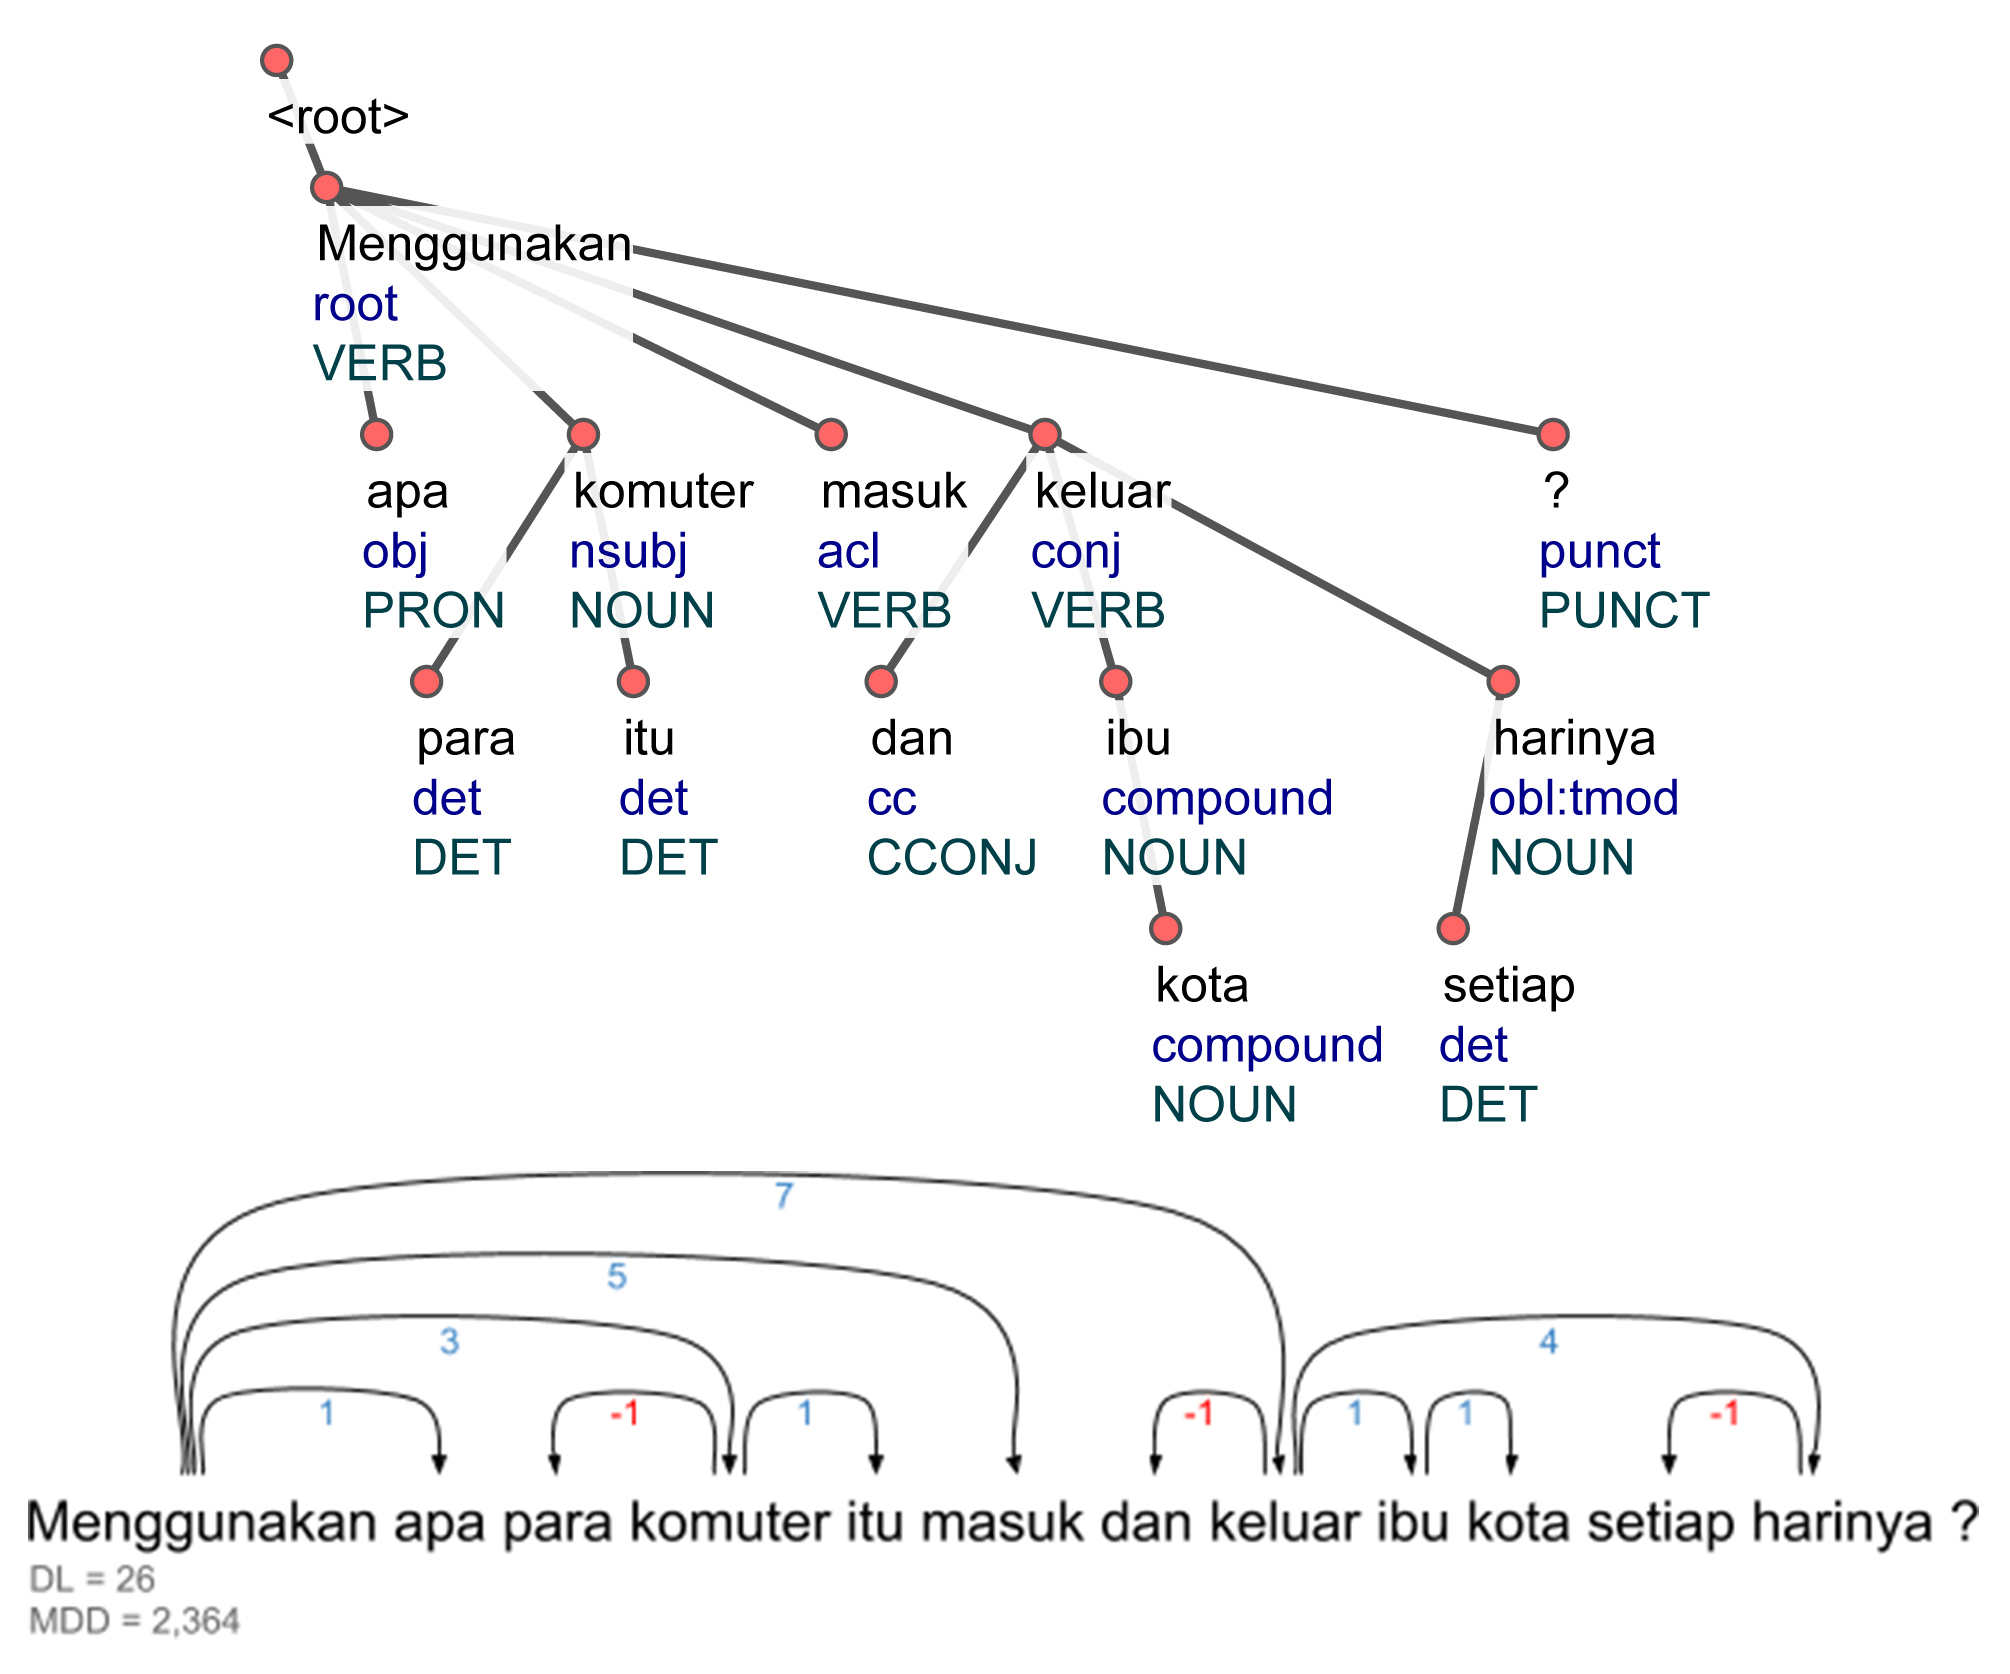
\includegraphics[width=.57\textwidth]{pics/ts7458.jpg} 
	\caption{Kalimat T\textit{akar}a pada data ragam tulis}
	\label{fig:ts7458} 
\end{figure}

Kalimat T\textit{akar}a (\pic~ref{fig:ts7458}) tetap mempertahankan valensi terhadap \textit{komuter} (aktor pelaku) dan \textit{apa} (pengganti obyek) namun konstruksinya tidak umum seperti halnya aktor pelaku mendahului verba dalam bahasa Indonesia. Contoh ini memberikan indikasi pemanfaatan kebebasan urutan kata dalam Bahasa Indonesia untuk menghindari bentuk relasi diakhiri induk dan tetap merealisasikan akar seawal mungkin. Penempatan klausa utama di awal kalimat lebih banyak ditemukan pada data ragam tulis dibandingkan ragam lisan. Penempatan klausa utama di awal kalimat ini menyebabkan akar verbal secara otomatis tetap berada di awal tanpa mengurangi valensi akar verbal tersebut. Namun, seiring jumlah konstituen yang semakin banyak dan struktur kalimat dengan klausa-klausa yang semakin kompleks, posisi akar verbal umumnya tidak pada posisi pertama meskipun masih pada rentang awal kalimat. Salah satu penyebab posisi akar sangat jarang ditemukan pada posisi pertama di kategori kalimat panjang adalah karena konstituen terikat berupa aktor pelaku umumnya direalisasikan sebelum akar verbal. Contoh strategi ini dapat dilihat pada kalimat T31b (\pic~\ref{fig:ts2081}) untuk data ragam tulis dan L31a (\pic~\ref{fig:ls1716}) untuk data ragam lisan.

%%-----------------------------------------------------------------------------%
\subsection{Pengurangan valensi akar pada klausa utama}
%%-----------------------------------------------------------------------------%
Sejumlah simpai pusat dalam kedua korpus data mengalami pengurangan valensi verbal yang mengakibatkan pengurangan panjang serta jarak dependensi. Hal ini berkaitan dengan temuan pengaruh panjang kalimat pada pembahasan sebelumnya yang menandakan kecenderungan jumlah konstituen yang lebih sedikit pada data ragam lisan. Strategi pengurangan valensi verbal ini juga ditemukan disertai penempatan akar di awal kalimat yang juga berkaitan dengan upaya menekan dependensi negatif yang berjarak jauh terutama pada kalimat panjang dalam data ragam lisan.

\begin{figure}
\centering

\begin{subfigure}{.49\linewidth}
  \centering
  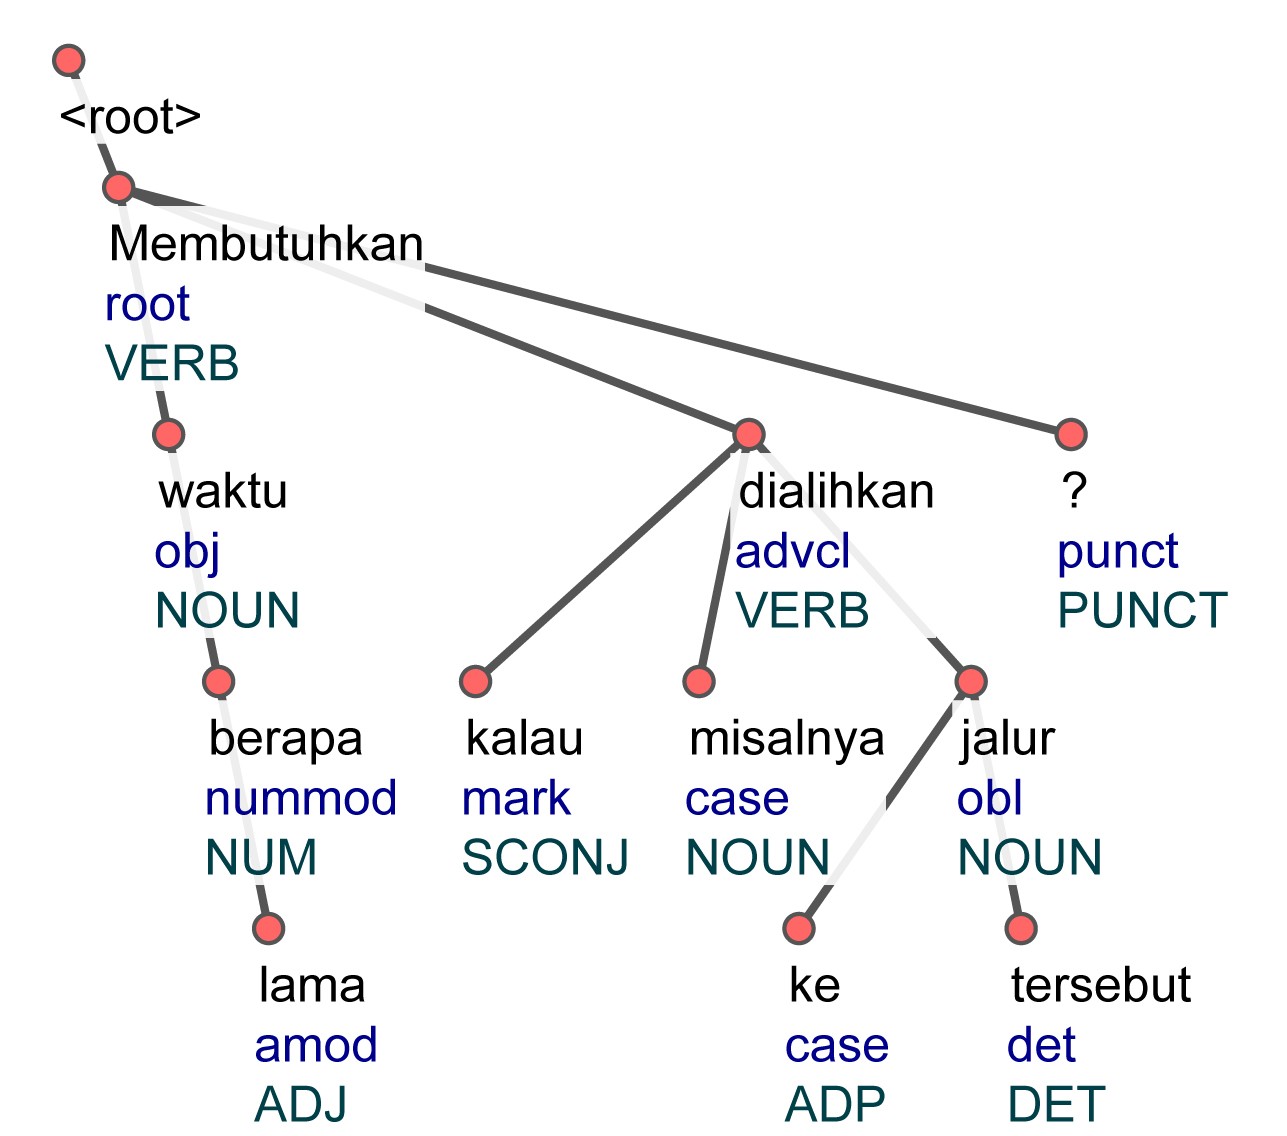
\includegraphics[width=1\linewidth] {pics/ls4820.jpg} 
	\caption{L\textit{akar}c}
	\label{fig:ls4820} 
\end{subfigure}
%
\begin{subfigure}{.41\linewidth}
  \centering
  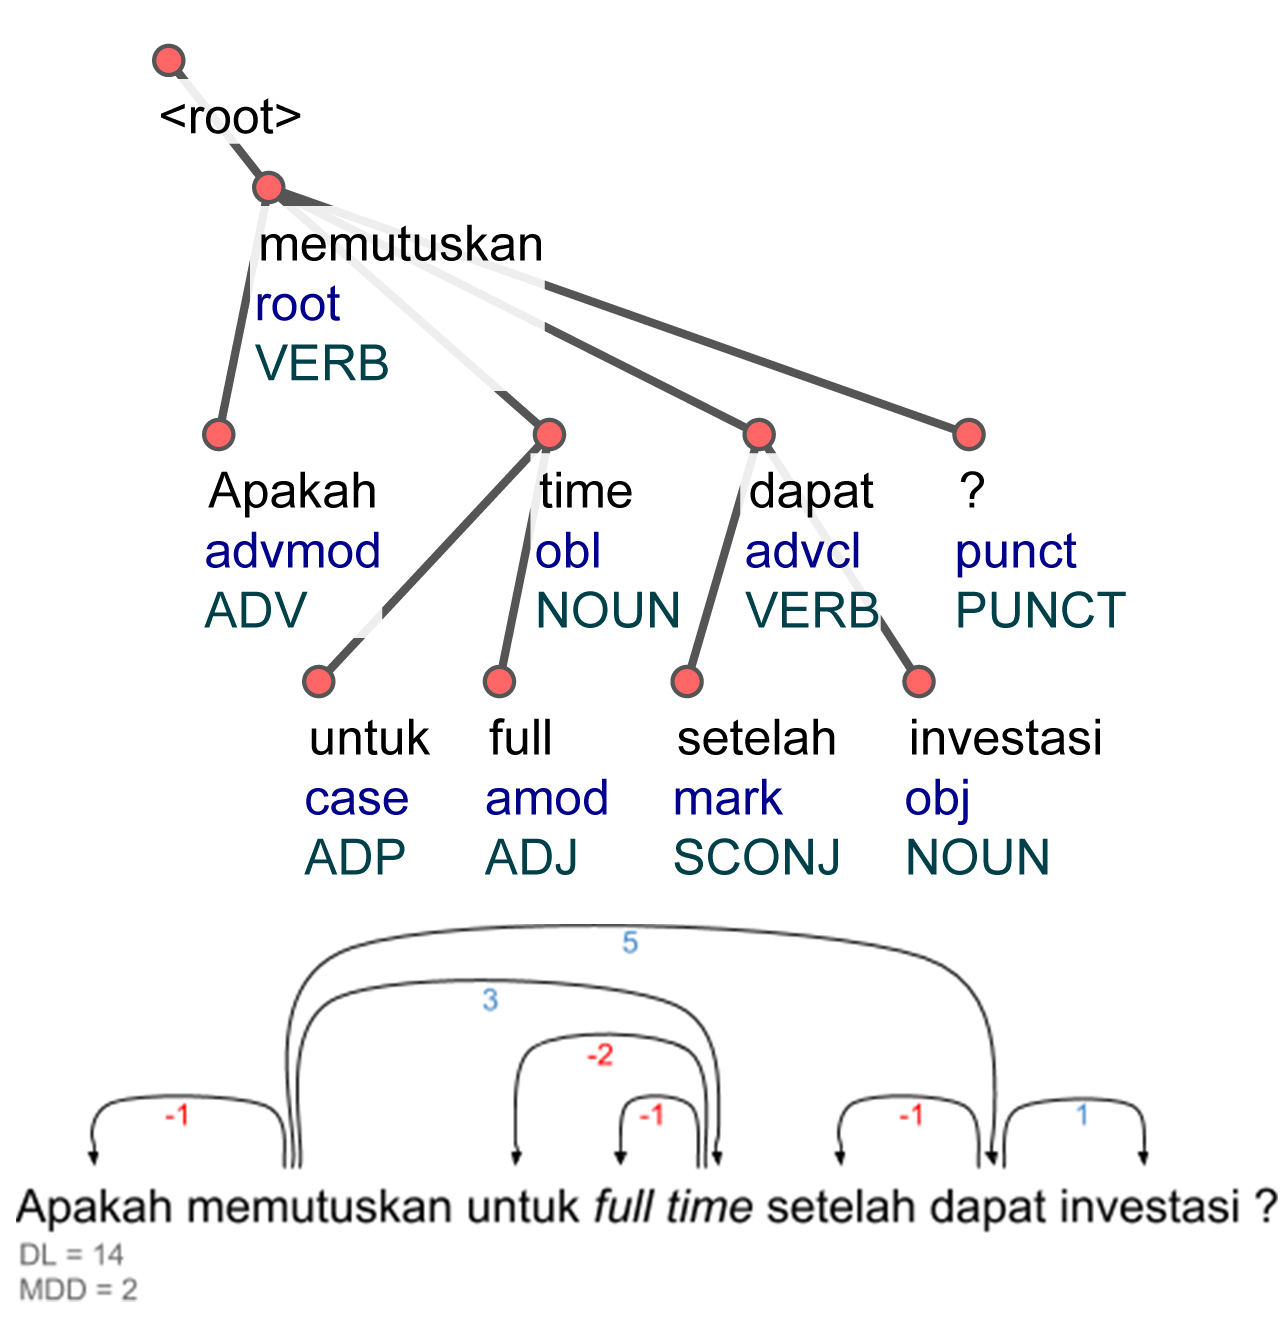
\includegraphics[width=1\linewidth]{pics/ls1435.jpg} 
	\caption{L\textit{akar}d}
	\label{fig:ls1435} 
\end{subfigure}
\caption{Contoh penempatan akar verbal dan klausa utama di awal kalimat tanpa pengurangan valensi verbal pada data ragam tulis}
\label{fig:rootvalensi}
\end{figure}

Pada kalimat L\textit{akar}c (\pic~\ref{fig:ls4820}), akar verbal \textit{membutuhkan} umumnya memiliki valensi sebanyak dua konstituen, yaitu aktor pelaku atau subyek berupa klausa dan obyek atau \textit{X membutuhkan Y}. Kata ini mengalami pengurangan valensi akar verbal sehingga yang muncul hanya obyek nomina \textit{waktu}. Meskipun demikian, akar \textit{membutuhkan} mengikat verba \textit{dialihkan} yang merupakan induk dari klausa keterangan. Pengurangan valensi pada data ragam lisan juga terjadi pada akar di posisi selain posisi pertama. Seperti pada kalimat L\textit{akar}d (\pic~\ref{fig:ls1435} yang juga mengalami pengurangan valensi berupa aktor pelaku untuk akar verbal \textit{memutuskan}. Kalimat L\textit{akar}e (\pic~\ref{fig:ls1265}), seperti juga kalimat L22 (\pic~\ref{fig:ls6521}), merupakan contoh yang mengalami pengurangan valensi verbal berupa aktor pelaku atau pronomina pada klausa utama maupun klausa terikatnya. Kalimat L\textit{akar}e tidak memunculkan pelengkap pada klausa \textit{X mengganti alat} dan/atau pada klausa \textit{supaya X tidak berebut ikan}.

\begin{figure}
	\centering 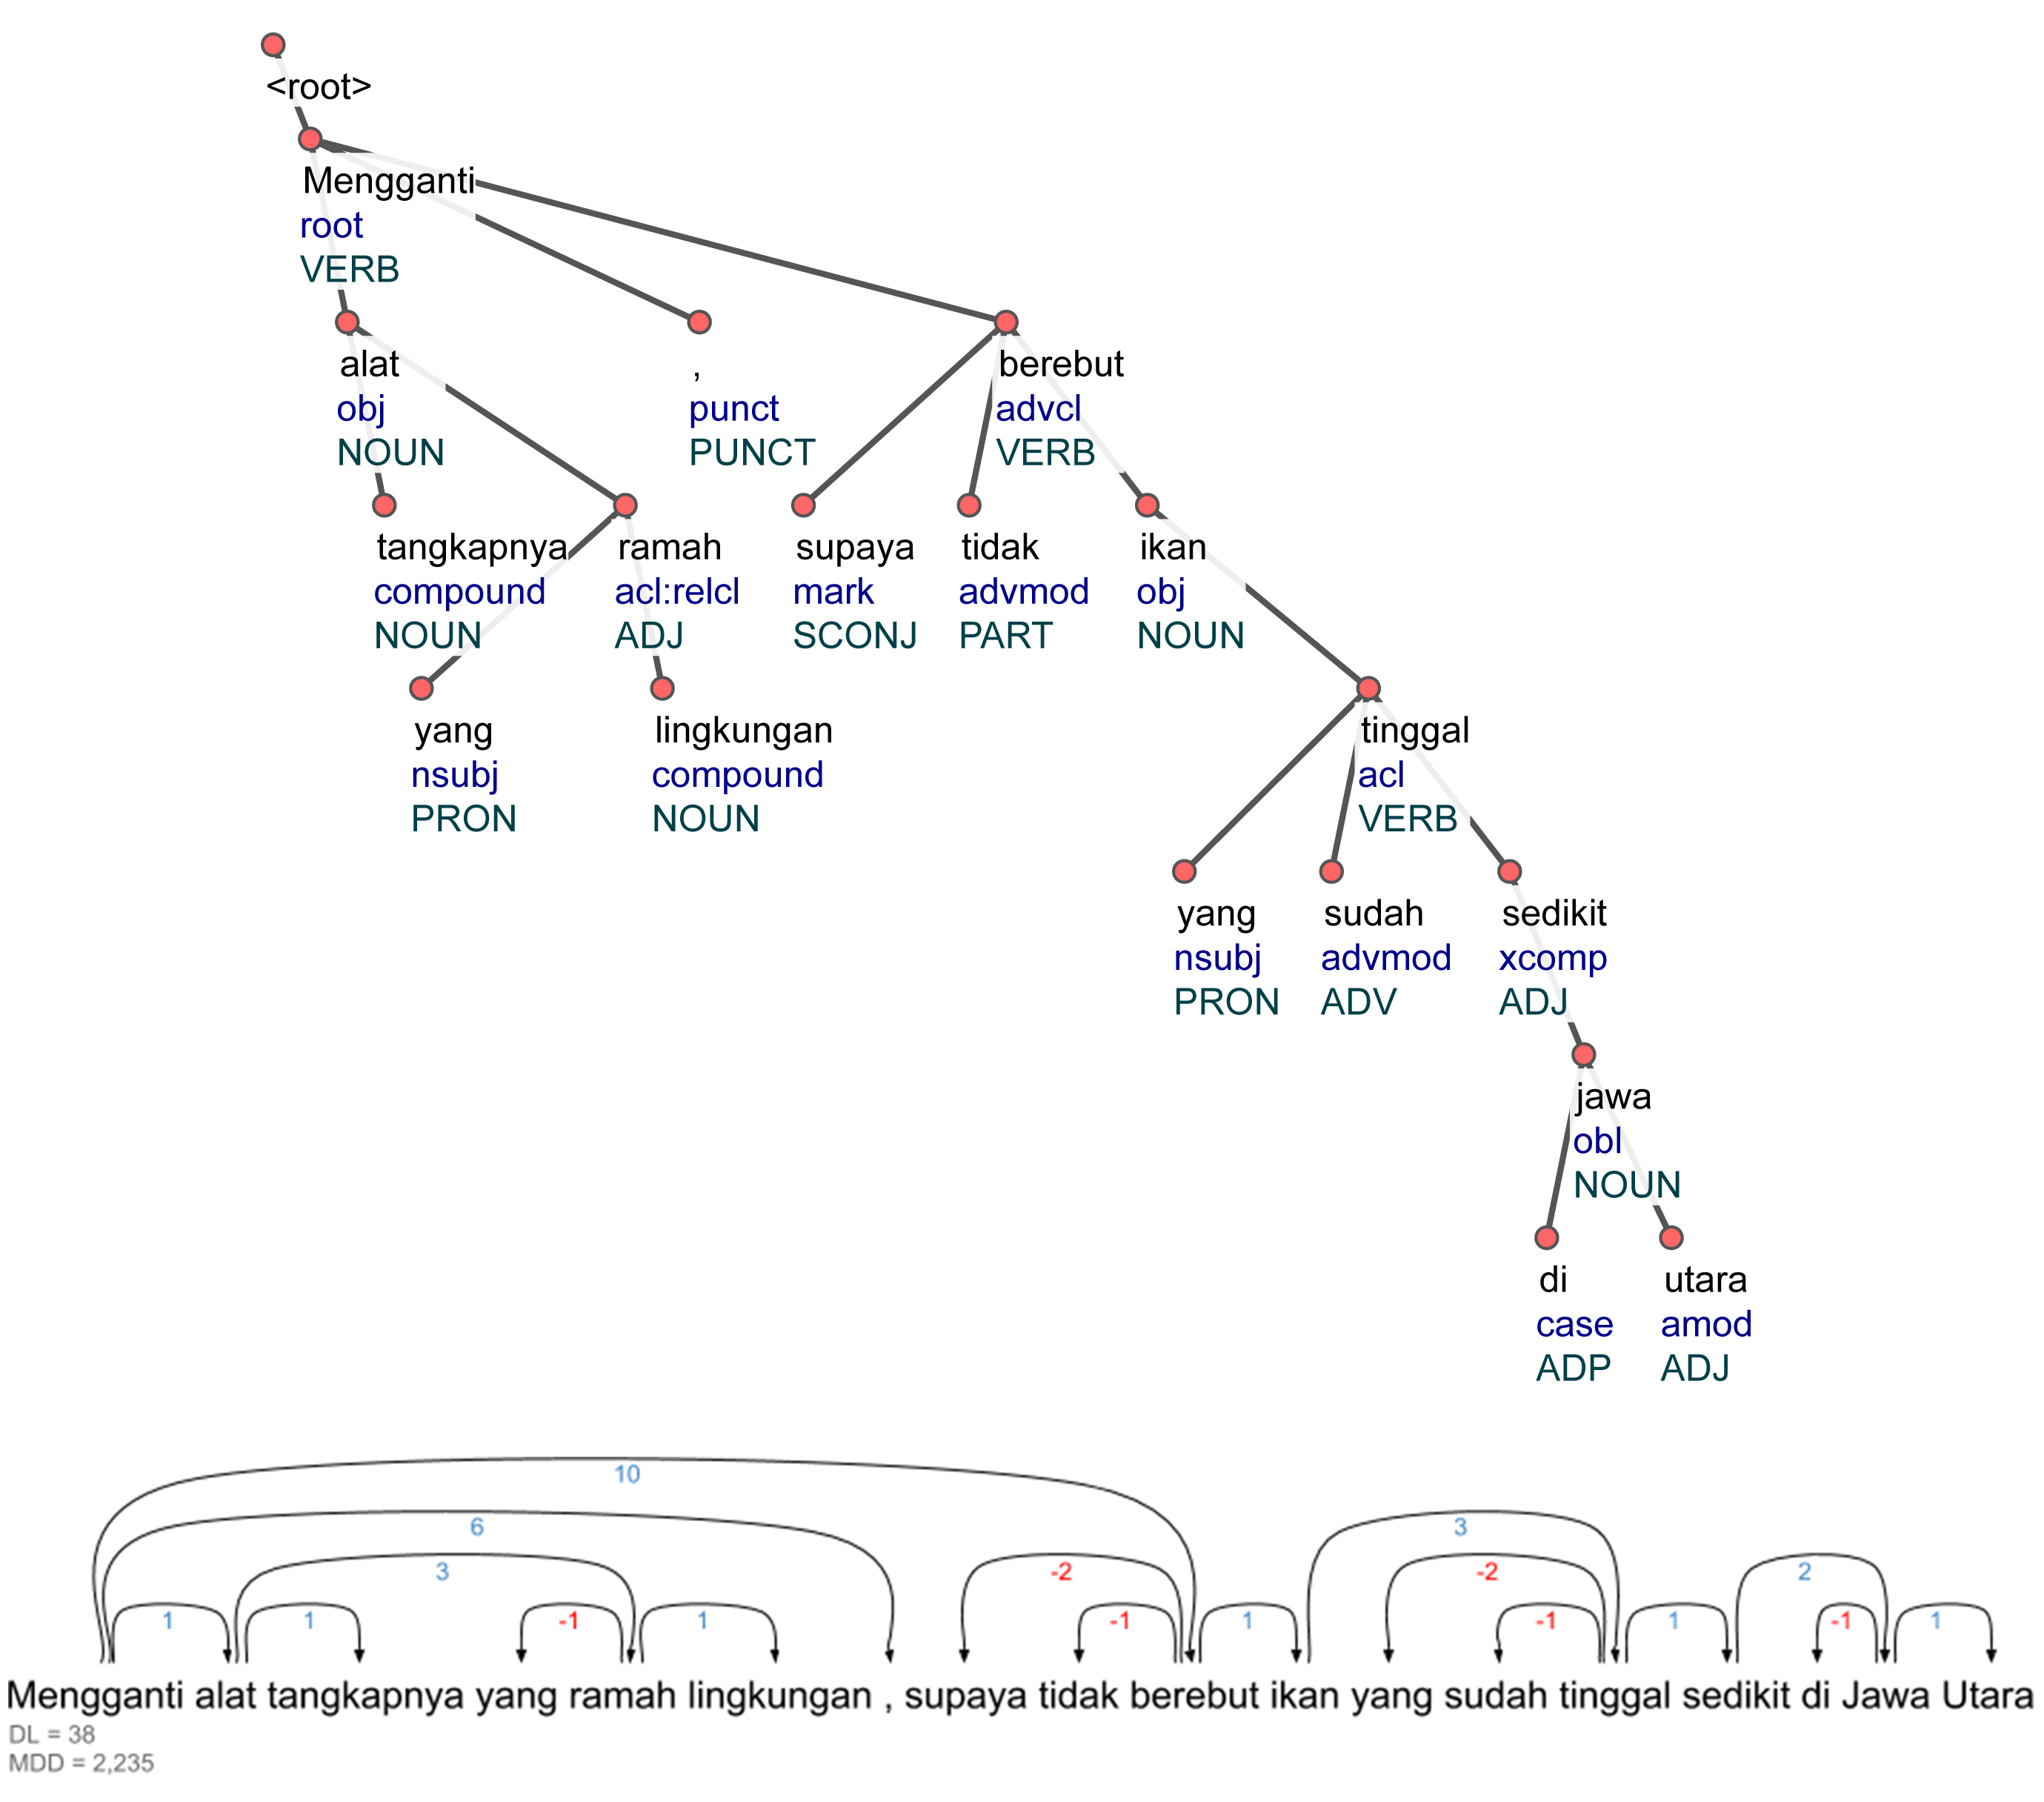
\includegraphics[width=0.9
	\textwidth] {pics/ls1265.jpg} 
	\caption{Kalimat L\textit{akar}e pada data ragam lisan}
	\label{fig:ls1265} 
\end{figure}

Strategi kalimat seperti ini muncul dalam wacana-wacana di mana konstituen yang direduksi dari valensi verbal sudah terlebih dahulu direalisasikan di kalimat-kalimat sebelumnya atau sudah dimengerti bersama tanpa harus direalisasikan dalam kalimat tertentu. Batasan penelitian ini hanya pada tataran kalimat sehingga tidak menganalisis hubungan dependensi yang terbentuk pada tataran wacana atau antarkalimat. Namun, asumsi ini menimbulkan pertanyaan untuk analisis dependensi lanjutan pada tataran wacana, yaitu bagaimana dan sejauh mana tautan dependensi yang terbentuk antarkalimat memungkinkan adanya pengurangan valensi verbal pada kalimat tertentu?

%%-----------------------------------------------------------------------------%
\subsection{Kecenderungan posisi induk terhadap konstituen terikat dalam kalimat}
%%-----------------------------------------------------------------------------%
Bagian analisis ini mencoba menjawab pertanyaan terkait direksionalitas induk atau arah tautan dependensi dan pengurangan valensi akar verbal pada simpai pusat. Pengurangan konstituen dalam kalimat atau preferensi terhadap kalimat pendek terutama pada ragam lisan tidak selalu berarti menandakan adanya pengurangan valensi sebuah konstituen. Pada penelitian-penelitian terdahulu banyak dilakukan eksplorasi terhadap reduksi leksikal lain seperti konjungsi, partikel, ataupun kata-kata lain yang bersifat berulang atau \textit{repetitive} (\citealp{jaeger2006redundancy, gildea2015human}). Penelitian ini memfokuskan pengurangan valensi pada simpai pusat dengan akar verbal yang merupakan tipe akar yang paling banyak ditemukan pada kedua korpus data. 

Seperti yang dibahas pada bab sebelumnya, direksionalitas induk dapat menyebabkan nilai dependensi tersebut menjadi positif atau negatif. Anotasi positif menandakan bentuk relasi induk sebelum konstituen terikat (diawali induk), sedangkan anotasi negatif menandakan bentuk relasi induk setelah konstituen terikat (diakhiri induk). Berdasarkan aturan struktur frasa dalam tata bahasa yang ada (\citealp{kridalaksana2002struktur, sneddon2010indonesian}), terdapat indikasi bahwa bahasa Indonesia tergolong bahasa yang memilih bentuk relasi diawali induk dibandingkan diakhiri induk atau \textit{head-final}. Namun, belum ada penelitian dengan skala cukup besar yang dapat memberikan informasi ini dengan memanfaatkan data tuturan nyata karena penerapannya dalam tuturan nyata dapat bersifat tidak gramatikal namun tetap diterima. Bentuk relasi diawali induk tidak selalu menjadi preferensi pada semua bahasa karena beberapa bahasa memiliki aturan tata bahasa yang menuntut induk muncul setelah konstituen terikat atau diakhiri induk. Meskipun belum ada konvensi dan bukti empiris yang menunjukkan bahwa bentuk diawali induk lebih memudahkan proses memori kerja, \cite{futrell2015large} menunjukkan bukti empiris bahwa bahasa-bahasa yang cenderung menggunakan bentuk relasi ini memiliki tingkat pengurangan jarak dependensi (DLM) lebih tinggi dibandingkan bahasa-bahasa yang cenderung menggunakan bentuk relasi diakhiri induk. 

Didukung oleh hasil penelitian ini, bahasa Indonesia menunjukkan kecenderungan terhadap bentuk relasi diawali induk pada keseluruhan kalimat (antarkonstituen yang memiliki tautan langsung) yang ditandai oleh konsistensi DL positif yang semakin besar dibandingkan DL negatif terutama pada kalimat yang memiliki jumlah konstituen lebih banyak. Namun, kecenderungan ini tidak terlalu jelas terlihat pada simpai pusat karena dari segi frekuensi, jumlah tautan dependensi negatif dan jumlah kalimat yang panjang dependensi negatifnya lebih besar ditemukan jauh lebih banyak terutama pada ragam lisan. Meskipun begitu, apabila jarak dependensi ikut diperhitungkan, terlihat adanya konsistensi untuk menekan panjang dan jarak dependensi negatif baik pada simpai pusat maupun keseluruhan kalimat. Secara otomatis, pergerakan DL positif yang semakin besar mengakibatkan penekanan bentuk relasi diakhiri induk yang ditandai oleh DL negatif. Bahkan, pada ragam lisan, ditemukan indikasi adanya ambang batas terhadap jarak dependensi untuk bentuk relasi diakhiri induk. Temuan ini memunculkan asumsi bahwa dalam bahasa Indonesia, bentuk relasi diawali induk lebih banyak digunakan penutur terutama pada relasi yang berjarak jauh. Hal ini juga menunjukkan indikasi bahwa bentuk ini lebih mudah diproduksi dan dipahami secara kognitif untuk penutur maupun penerima informasi. Penyebab adanya perbedaan kecenderungan frekuensi pada simpai pusat dan keseluruhan kalimat berkaitan dengan tinjauan kognitif dan persepsi manusia yang berada di luar batasan penelitian ini. Penelitian lebih lanjut yang dapat memperlihatkan bukti empiris dibutuhkan untuk mendukung hipotesis ini dan untuk mengukur seberapa besar dampak bentuk relasi diawali induk sehingga dapat memudahkan proses memori kerja. 

Analisis kualitatif untuk melihat lebih dalam bagaimana strategi yang mendukung preferensi bentuk relasi diawali induk ini dilakukan dengan meninjau simpai-simpai pusat kalimat yang memiliki akar verbal pada kedua korpus. Secara umum, ditemukan dua strategi terkait direksionalitas induk dan valensi akar verbal, yaitu penempatan akar dan klausa utama di awal kalimat dan pengurangan valensi akar verbal pada klausa utama. Penempatan akar dan klausa utama di awal kalimat sangat umum ditemukan pada semua klasifikasi dalam korpus data ragam tulis. Namun, posisinya sedikit bergeser ke tengah kalimat seiring dengan semakin banyaknya jumlah konstituen. Hal ini dikarenakan penempatan klausa utama yang hampir selalu berada di posisi awal kalimat pada data ragam tulis. Sementara, pengurangan valensi akar verbal hampir tidak ditemukan pada data ragam tulis yang mungkin disebabkan oleh karakter wacananya yang bersifat lebih formal dibandingkan dengan ragam lisan. 

Pengurangan valensi ini secara langsung berakibat pada pengurangan konstituen secara keseluruhan, sehingga dapat dikaitkan dengan temuan adanya preferensi untuk menggunakan kalimat dengan jumlah konstituen yang lebih sedikit pada ragam lisan, terutama pada klasifikasi kalimat pendek dan menengah. Beberapa kasus pengurangan valensi akar verbal ini juga ditemukan disertai dengan penempatan posisi akar di awal kalimat ragam lisan. Pada kasus yang lain, pengurangan valensi ini juga ditemukan pada klausa terikat di dalam kalimat tersebut. Mulai pada panjang kalimat tertentu, akar verbal yang mengikat aktor pelaku dalam valensinya tidak ditemukan pada posisi pertama dan aktor pelaku hampir selalu direalisasikan sebelum akar verbal atau didahului oleh konstituen dan klausa terikat. Pengurangan valensi subyek yang berupa kata penuh pada simpai pusat akar verbal tidak ditemukan apabila klausa utama didahului klausa lain, namun pengurangan valensi subyek yang berupa pronomina pengganti pada simpai dengan induk verbal ditemukan apabila klausa utama juga mengalami pengurangan valensi subyek. Untuk meninjau lebih dalam signifikansi temuan pengurangan valensi pada kondisi tersebut memerlukan pendekatan kuantitatif yang menuntut adanya sumber daya kamus atau leksikon valensi. Tinjauan lebih lanjut dengan memanfaatkan leksikon valensi dapat memberikan gambaran lebih dalam mengenai kognisi manusia terkait struktur kalimat yang dikonstruksi dan dapat memberikan masukan terhadap penggunaan tata bahasa yang memudahkan komunikasi serta proses memori kerja.

%%-----------------------------------------------------------------------------%
%\section{thesis.tex}
%%-----------------------------------------------------------------------------%
%Berkas ini berisi seluruh berkas Latex yang dibaca, jadi bisa dikatakan sebagai 
%berkas utama. Dari berkas ini kita dapat mengatur bab apa saja yang ingin 
%kita tampilkan dalam dokumen.
%
%
%%-----------------------------------------------------------------------------%
%\section{laporan\_setting.tex}
%%-----------------------------------------------------------------------------%
%Berkas ini berguna untuk mempermudah pembuatan beberapa template standar. 
%Anda diminta untuk menuliskan judul laporan, nama, npm, dan hal-hal lain yang 
%dibutuhkan untuk pembuatan template. 
%
%
%%-----------------------------------------------------------------------------%
%\section{istilah.tex}
%%-----------------------------------------------------------------------------%
%Berkas istilah digunakan untuk mencatat istilah-istilah yang digunakan. 
%Fungsinya hanya untuk memudahkan penulisan.
%Pada beberapa kasus, ada kata-kata yang harus selalu muncul dengan tercetak 
%miring atau tercetak tebal. 
%Dengan menjadikan kata-kata tersebut sebagai sebuah perintah \latex~tentu akan 
%mempercepat dan mempermudah pengerjaan laporan. 
%
%
%%-----------------------------------------------------------------------------%
%\section{hype.indonesia.tex}
%%-----------------------------------------------------------------------------%
%Berkas ini berisi cara pemenggalan beberapa kata dalam bahasa Indonesia. 
%\latex~memiliki algoritma untuk memenggal kata-kata sendiri, namun untuk 
%beberapa kasus algoritma ini memenggal dengan cara yang salah. 
%Untuk memperbaiki pemenggalan yang salah inilah cara pemenggalan yang benar 
%ditulis dalam berkas hype.indonesia.tex.
%
%
%%-----------------------------------------------------------------------------%
%\section{pustaka.tex}
%%-----------------------------------------------------------------------------%
%Berkas pustaka.tex berisi seluruh daftar referensi yang digunakan dalam 
%laporan. 
%Anda bisa membuat model daftar referensi lain dengan menggunakan bibtex.
%Untuk mempelajari bibtex lebih lanjut, silahkan buka 
%\url{http://www.bibtex.org/Format}. 
%Untuk merujuk pada salah satu referensi yang ada, gunakan perintah \bslash 
%cite, e.g. \bslash cite\{latex.intro\} yang akan akan memunculkan 
%\cite{latex.intro}
%
%
%%-----------------------------------------------------------------------------%
%\section{bab[1 - 6].tex}
%%-----------------------------------------------------------------------------%
%Berkas ini berisi isi laporan yang Anda tulis. 
%Setiap nama berkas e.g. bab1.tex merepresentasikan bab dimana tulisan tersebut 
%akan muncul. 
%Sebagai contoh, kode dimana tulisan ini dibaut berada dalam berkas dengan nama 
%bab4.tex. 
%Ada enam buah berkas yang telah disiapkan untuk mengakomodir enam bab dari 
%laporan Anda, diluar bab kesimpulan dan saran. 
%Jika Anda tidak membutuhkan sebanyak itu, silahkan hapus kode dalam berkas 
%thesis.tex yang memasukan berkas \latex~yang tidak dibutuhkan;  contohnya 
%perintah \bslash include\{bab6.tex\} merupakan kode untuk memasukan berkas 
%bab6.tex kedalam laporan.
%
